% ============================================
% Chapter 5 – Implementation
% ============================================

\chapter{Implementation}
\justifying

This chapter describes the practical implementation of the Lets Go Ride Sharing App ride-sharing and recommendation system. It explains how the architectural design and models presented in Chapter 4 were translated into working modules, algorithms, user interfaces, and deployment components. The implementation follows the modular design and incremental delivery approach outlined earlier.

% -------------------------------------------------
% 5.1 Development Environment
% -------------------------------------------------

\section{Development Environment}

The development environment for the Lets Go Ride Sharing App system was selected to support Flutter mobile development, a Django backend, PostgreSQL database management, and template-based Admin pages.

\textbf{IDE and Tools:}

Visual Studio Code – main editor for writing Flutter (Dart) and Django (Python).

Android Studio – for Android emulator testing and Flutter layout debugging.

Figma – UI/UX Design \& Prototyping.

Postman – HTTP Endpoint Testing for Backend Integration Testing.
\begin{itemize}
    \item Git \& GitHub – Version control and collaboration (including issue tracking).
\end{itemize}
Supabase Dashboard – Database Inspection and Storage Bucket Management for Supabase PostgreSQL and Supabase Storage.

Programming Languages and Frameworks:

Frontend (Mobile): Dart and Flutter for cross-platform mobile screens.
\begin{itemize}
    \item Frontend: HTML, CSS, and JavaScript.
    \item Database: SQLite.
    \item Authentication: Session-based authentication with Django sessions with the user id saved in the \texttt{request.session['user\_id']} property.
    \item Notifications: Notification logic for the backend and push delivery via FCM as well as email/SMS support where set up.
\end{itemize}
Database: PostgreSQL on Supabase.
\begin{itemize}
    \item Storage: Uploaded images and documents are stored in Supabase Storage.
    \item Haversine Distance: An algorithmic formula for calculating distances between two locations.
\end{itemize}

Backend support chatbot as a local utility within the Django project that can optionally include LLM support in the event that environment variables are set.

Operating System and Hardware:

Development OS: Ubuntu, Windows 10 and Windows 11 have been used for development and testing.
\begin{itemize}
    \item Backend Hosting Environment: Cloud deployment of backend and Admin pages (Django).
    \item Hardware:
        \begin{itemize}
            \item Modern multi-core processor and 16+ GB RAM machines for development.
            \item Application validation (Android and iOS) using mobile test devices and emulators.
        \end{itemize}
\end{itemize}

% -------------------------------------------------
% 5.2 Core Module Implementation
% -------------------------------------------------

\section{Core Module Implementation}

This section describes the implementation of the main modules of the Lets Go Ride Sharing App system. Each module was designed as a standalone feature or a screen flow within the Flutter app, maintaining the code structure and making it easier to maintain.

\subsection{Module 1: Authentication \& Verification Module}

This is used to manage user registration, login, OTP verification, password reset and Admin review of documents.

\textbf{Key Functionalities:}
\begin{itemize}
    \item User Registration by email, phone, CNIC and (optional) license/bank details.
    \item Upload profile images, CNIC images, driver license images, vehicle documents to Supabase Storage.
    \item OTP generation and verification for account verification \& password reset flow.
    \item Logging in automatically to the session once successful.
    \item Administrator pages to see pending validations and approve, reject or ban users.
\end{itemize}

\textbf{Important Classes/Functions:}
\begin{itemize}
    \item User profile database for passenger \& driver data.
    \item User document/image fields stored in user profile model, uploaded assets stored in Supabase Storage with reference through stored URLs.
    \item Web-based helpers for generating and verifying OTPs, with server side cache/state and configured delivery utilities for email/SMS.
    \item Django function-based views were mapped on the following routes: \texttt{/signup/}, \texttt{/login/}, \texttt{/send\_otp/}, \texttt{/verify\_otp/}, and \texttt{/reset\_password/}.
    \item The Flutter screens that are being registered are \texttt{RegistrationScreen}, \texttt{OTPScreen} and \texttt{DocumentUploadScreen}.
\end{itemize}

\textbf{Integration:} interacts with the notification layer for OTP delivery and Supabase Storage for document uploads. The updating of the user status and triggering of the corresponding notifications are carried out due to admin actions.

\subsection{Module 2: Ride Management Module}

\textbf{Aim:} To allow drivers to develop, edit and publish rides as well as control stops on the ride and ride parameters.

\textbf{Key Functionalities:}
\begin{itemize}
    \item Map-based route editor with the ability to create start, intermediate and end stops.
    \item The fare calculation is done based on the distance of the route, type of the vehicle and ride parameters.
    \item Availability of departure time and seats, gender preference and the availability for negotiation.
    \item Adding the ride to the passenger discovery pages and updating the ride information using a form in the backend.
\end{itemize}

\textbf{Important Classes/Functions:}
\begin{itemize}
    \item Ride model using route and stop data.
    \item FareCalculator is a utility to calculate the fare distance, based on Haversine distance, and route metadata.
    \item Django views in \texttt{/create\_route/}, \texttt{/create\_trip/}, and \texttt{/trips/<trip\_id>/...}.
    \item These screens should be flutter screens that are created as follows: \texttt{CreateRideScreen}, \texttt{MyRidesScreen}, and \texttt{RideDetailsScreen}.
\end{itemize}

\textbf{Integration:} Saves data for rides in PostgreSQL, provides fare calculation helpers for routes and distance, and provides access to the ride data to the passenger search and booking flows.

\subsection{Module 3: Booking \& Payment Module}

\textbf{Objective:} To enable passengers to locate, check, reserve and confirm trips, as well as to lock the seats, negotiate and manually confirm payments.

\textbf{Key Functionalities:}
\begin{itemize}
    \item Search for rides by origin, destination, date and gender preference.
    \item Choose pick up and drop off stops from a driver route.
    \item Prevent overbooking by locking seats when booking.
    \item Accept, reject, cancel and confirm bookings.
    \item Manual payment flow in which the passenger indicates that payment is made and the driver checks it.
\end{itemize}

\textbf{Important Classes/Functions:}
\begin{itemize}
    \item Requested, accepted, rejected, cancelled, completed booking model with states.
    \item Payment model that is based on bookings.
    \item Endpoints that are related to Django, like \texttt{/ride-booking/<trip\_id>/}, \texttt{/bookings/<booking\_id>/payment/submit/}, and \texttt{/bookings/<booking\_id>/payment/confirm/}.
    \item The following screens will be fluttered: \texttt{SearchRidesScreen}, \texttt{BookingScreen} and \texttt{PaymentScreen}.
\end{itemize}

\textbf{Integration:} Communicates with notification layer for alerts and updates on state changes after booking rides.

\subsection{Module 4: Live Tracking \& Safety Module}

In this Module 4: Live Tracking \& Safety Module, you will learn how to track animals in the field and how to keep them safe and sound.

\textbf{Purpose:} Frequency update support with HTTP near real-time ride tracking, pickup code verification, SOS emergency and ride completion support.

\textbf{Key Functionalities:}
\begin{itemize}
    \item Location updates are transmitted via HTTP endpoints on the client via polling or periodic updates.
    \item Passenger boarding is verified by code picking and code verification.
    \item SOS incidents alert through e-mail/SMS workflows and create shareable tracking links or tokens.
    \item Data of the incidents and tracking data are saved for review in the Admin pages.
\end{itemize}

\textbf{Important Classes/Functions:}
\begin{itemize}
    \item \texttt{PickupCodeService} for creating and verifying pickup codes.
    \item \texttt{SOSIncident} and \texttt{SOSService} for emergency handling.
    \item \texttt{TripShareToken} is a link to share your trip.
    \item Endpoints like \texttt{/pickup-code/verify/}, \texttt{/incidents/sos/}, \texttt{/incidents/sos/share/<token>/...} and \texttt{/trips/<trip\_id>/share/...} are examples of these.
    \item For the live tracking screen and pick up code entry screen, flutter screens were created.
\end{itemize}

\textbf{Integration:} Integrates Haversine distance logic for location-based checks, backend notification logic for alerts, and Admin pages to monitor incidents.

\subsection{Module 5: Admin Portal Module}

\textbf{Goal:} Web based administration pages to verify use, to resolve disputes, to review incidents and monitor system usage.

\textbf{Key Functionalities:}
\begin{itemize}
    \item Lists of users with pager and filter by verification status.
    \item Record and accept/reject/ban.
    \item Dispute resolution, including evidence including chat logs, location history and uploaded images.
    \item Resolution workflow including notes and notifications of parties involved.
    \item A view of important operational information on the dashboard.
\end{itemize}

\textbf{Important Classes/Functions:}
\begin{itemize}
    \item Admin pages and views using the Django template system.
    \item Handling Disputes and Verification views.
    \item The VerificationService is a service used for the document review logic.
    \item Normal Django templates and Bootstrap styling are used for the dashboard widgets.
\end{itemize}

\textbf{Integration:} Pulls in data from all the core modules and notifies when the Admin changes a user or dispute state.

% -------------------------------------------------
% 5.3 Algorithmic Implementation
% -------------------------------------------------

\section{Algorithmic Implementation}

This section details the formal logic used in the core modules of the Lets Go Ride Sharing App system. The algorithms cover user onboarding, ride management, booking constraints, live tracking, safety handling, chatbot support, route logic, notifications, blocking, and ratings.

\subsection{Algorithm 1: User Registration \& Verification}

This algorithm processes the user onboarding, stores the user who has successfully signed in to a Django session and activates accounts after verifies the OTP.

\begin{breakablealgorithm}
\caption{This algorithm deals with the process of user registration and OTP verification.This algorithm is related to user registration and OTP verification.}
\textbf{Input:} User data (Email, Phone, Password, User role) \\
\textbf{Output:} Verification status and session state
\begin{algorithmic}[1]
\State TO ADD A USER TO THE SITE, YOU NEED TO CALL THE FOLLOWING FUNCTION:
\Function{RegisterUser}{$email, phone, password, role$}
    \If{\Call{CheckExists}{$email$} \textbf{or} \Call{CheckExists}{$phone$}}
        \State \Return Error("User already exists")
    \EndIf
    \State $user \gets$ \Call{CreateUserRecord}{$email, phone, password, role$}
    \State $otp \gets$ \Call{GenerateOTP}{6}
    \State \Call{StoreOTP}{$user.id, otp, 5\text{ minutes}$}
    \State \Call{SendOTP}{$phone, email$}
    \State \Return "OTP sent"
\EndFunction

\Function{VerifyOTPAndLogin}{$user, otp$}
    \If{\Call{ValidateOTP}{$user.id, otp$}}
        \State \Call{SetSession}{$\text{request.session['user\_id']} = user.id$}
        \State \Return "Verified"
    \Else
        \State \Return Error("Invalid OTP")
    \EndIf
\EndFunction
\end{algorithmic}
\end{breakablealgorithm}

\textbf{Explanation:} The system will check the uniqueness of the user, then create a code called OTP and send it via a text message to the user's mobile phone. Uses the configured notification channel, and updates the verified user's id in the Django session after successful login/verification.

\subsection{Algorithm 2: Ride Creation \& Fare Calculation}

This algorithm is run when a drive is created or updated. It determines the distance of the route uses stored stop points, and calculates fare based on local business rules.

\begin{breakablealgorithm}
\caption{Ride Creation and Fare Calculation}
\textbf{Input:} Ordered stops $W$, Vehicle type $V$ \\
\textbf{Input:} Fares and route number \\
\textbf{Output:} Ride record and estimated fare
\begin{algorithmic}[1]
\Function{CreateRide}{$W, V$}
    \State $total\_distance \gets 0$
    \For{$i \gets 1$ \textbf{to} $\Call{Length}{W} - 1$}
        \State $segment \gets$ \Call{HaversineDistance}{$W[i], W[i+1]$}
        \State $total\_distance \gets total\_distance + segment$
        \EndFor
    \State $base\_rate \gets$ \Call{GetBaseRate}{}
    \State $multiplier \gets$ \Call{GetVehicleMultiplier}{$V$}
    \State $fare \gets total\_distance \times base\_rate \times multiplier$
    \State $ride \gets$ \Call{SaveRideRecord}{$W, V, fare$}
    \State \Return $ride, fare$
\EndFunction
\end{algorithmic}
\end{breakablealgorithm}

\textbf{Explanation:} The fare is not based on the distance traveled but on distance on the route and also on the rules for the vehicles. An external routing service as the main computation backend.

\subsection{Algorithm 3: Ride Booking \& Seat Locking}

This algorithm handles requests for booking, avoids the possibility of overbooking, and ensures seats are booked according to the rules availability.

\begin{breakablealgorithm}
\caption{Ride Booking and Seat Locking}
\textbf{Input:} Passenger ID, Trip ID, S, Seats requested \\
\textbf{Output:} Booking status
\begin{algorithmic}[1]
\Function{CourseRide}{$P, T$}
    \State \Call{BeginDBTransaction}{}
    \State $trip \gets$ \Call{FetchTripWithLock}{$T$}
    \If{the number of seats available in the trip, $trip.available\_seats$, is less than $S$}
        \State \Call{RollbackDBTransaction}{}
        \State \Return "The number of seats is insufficient.Return "The number of seats is insufficient."
    \EndIf
    \State \Return Success("Booking requested")
\EndFunction
\end{algorithmic}
\end{breakablealgorithm}

\textbf{Explanation:} A database transaction is used to avoid simultaneous bookings from removing the book. The same seating capacity.

\subsection{Algorithm 4: Live Tracking \& Pickup Code Verification}

That is an algorithm that handles periodic updates of location via HTTP-based tracking and produces a pickup code when the driver gets to the pickup area.

\begin{breakablealgorithm}
\small
\caption{Live Tracking and Pickup Code Verification}
\textbf{Input:} The driver location is located at LD, the passenger pickup location is located at LP, and the trip ID is T. \\
\textbf{Output:} Track and status code/pickup code is being tracked.
\begin{algorithmic}[1]
\Function{UpdateLiveLocation}{$L_D, L_P, T$}
    \State $distance \gets$ \Call{HaversineDistance}{$L_D, L_P$}
    \State \Call{SaveLocationUpdate}{$T, L_D$}
    \If{distance is less or equal to 100 meters and it doesn't exist \Call{PickupCodeExists}{$T$}}
        \State $code \gets$ \Call{GenerateSecureCode}{4}
        \State \Call{SavePickupCode}{$T, code$}
        \State \Call{NotifyPassenger}{$T, code$}
    \EndIf
    \State \Return $distance$
\EndFunction

\Function{VerifyPickupCode}{$T, code$}
    \If{\Call{MatchPickupCode}{$T, code$}}
        \State \Call{UpdateTripStatus}{$T, \text{"IN\_PROGRESS"}$}
        \State \Return Success("Code verified")
    \Else
        \State \Return Error("Invalid pickup code")
    \EndIf
\EndFunction
\end{algorithmic}
\end{breakablealgorithm}

\textbf{Explanation:} The system stores periodic GPS updates via HTTP requests and verifies the pickup code prior to the trip can be moved to the in-progress state.

\subsection{Algorithm 5: SOS Escalation Logic}

This algorithm notifies contacts, logs SOS incidents and creates a shareable tracking token.

\begin{breakablealgorithm}
\small
\caption{Link Generation Considerations for SOS Incident Handling}
\textbf{Input:} User ID $U$, Trip ID $T$, Current location $L$ \\
\textbf{Result:} Incident record and share token
\begin{algorithmic}[1]
\Function{HandleSOS}{$U, T, L$}
    \If{\Call{SOSAlreadyActive}{$T$}}
        \State \Return
    \EndIf
    \State \Call{CreateSOSIncident}{$U, T, L$}
    \State $token \gets$ \Call{GenerateShareToken}{$T$}
    \State \Call{SaveShareToken}{$T, token$}
    \State \Call{NotifyEmergencyContacts}{$U, L$}
    \State \Call{NotifyAdminPages}{$T, L$}
    \State \Call{SendEmailSMS}{$U, T, L, token$}
\EndFunction
\end{algorithmic}
\end{breakablealgorithm}

\textbf{Explanation:} The SOS flow maintains an incident log that is available for future reference and notifies on-call personnel by sending alerts. sends the configured notification channels and creates a tracking token to be shared safely location sharing.

\subsection{Algorithm 6: Ride Suggestion Helper}

This algorithm summarizes a lightweight ride suggestion approach based on metadata similarity and recent user history.

\begin{breakablealgorithm}
\caption{Ride Suggestion Helper}
\textbf{Input:} User ID $U$, list of available rides $A$ \\
\textbf{Output:} Ranked ride suggestions
\begin{algorithmic}[1]
\Function{RecommendRides}{$U, A$}
    \State $history \gets$ \Call{GetRecentTrips}{$U$}
    \If{$history$ is empty}
        \State \Return \Call{GetPopularRides}{}
    \EndIf
    \State $scores \gets$ \Call{ScoreByMetadataSimilarity}{$history, A$}
    \State \Return \Call{SortDescending}{$scores$}
\EndFunction
\end{algorithmic}
\end{breakablealgorithm}

\textbf{Explanation:} The recommendation helper uses local trip metadata and simple similarity scoring rather than an external production ML service.

\subsection{Algorithm 7: Route ETA Calculation}

This algorithm computes an estimated distance and duration between two stops on a stored route.

\begin{breakablealgorithm}
\caption{Dynamic Route Segment ETA Calculation}
\textbf{Input:} Trip ID $T$, pickup order index $O_P$, drop-off order index $O_D$ \\
\textbf{Output:} Total duration and distance
\begin{algorithmic}[1]
\Function{CalculateRouteDuration}{$T, O_P, O_D$}
    \State $segments \gets$ \Call{LoadTripSegments}{$T$}
    \State $total\_duration \gets 0$
    \State $total\_distance \gets 0$
    \For{\textbf{each} $seg \in segments$}
        \If{$seg.from\_order \geq O_P$ \textbf{and} $seg.to\_order \leq O_D$}
            \State $total\_duration \gets total\_duration + seg.duration$
            \State $total\_distance \gets total\_distance + seg.distance$
        \EndIf
    \EndFor
    \If{$total\_duration = 0$}
        \State \Return Null
    \EndIf
    \State \Return \Call{Ceil}{$total\_duration$}, $total\_distance$
\EndFunction
\end{algorithmic}
\end{breakablealgorithm}

\textbf{Explanation:} The ETA is derived from stored trip segment data, which avoids repeatedly depending on an external routing service for every passenger request.

\subsection{Algorithm 8: Trip Archiving and State History}

This algorithm stores completed trip data and keeps a compact audit trail of the trip lifecycle.

\begin{breakablealgorithm}
\caption{Trip Archiving and State History}
\textbf{Input:} Trip object $T$, completion time $t_{end}$ \\
\textbf{Output:} Archived status
\begin{algorithmic}[1]
\Function{ArchiveTrip}{$T, t_{end}$}
    \If{the time difference between the current time and tend is less than 24 hours, then}
        \State \Return False
    \EndIf
    \If{\Call{HasPendingPayment}{$T$}}
        \State \Return False
    \EndIf
    \State \Call{MarkTripArchived}{$T$}
    \State \Call{StoreTripHistory}{$T$}
    \State \Call{KeepAuditLog}{$T$}
    \State \Return True
\EndFunction
\end{algorithmic}
\end{breakablealgorithm}

\textbf{Explanation:} After the operational workflow is completed, the finished trips can be archived - The audit log and status history are kept for future reference.

\subsection{Algorithm 9: Polyline Decoding for Route Geometry}

This algorithm will decode route geometry that is encoded back from mapping utilities to coordinate pairs.

\begin{breakablealgorithm}
\small
\caption{Route Polyline Decoding}
\textbf{Input:} Encoded route string $E$ \\
\textbf{Output:} List of coordinate pairs
\begin{algorithmic}[1]
\Function{DecodePolyline}{$E$}
    \State $coords \gets [~]$
    \State $index \gets 0$, $lat \gets 0$, $lng \gets 0$
    \While{$index < \Call{Length}{E}$}
        \State $dlat \gets$ \Call{DecodeNextVarint}{$E, index$}
        \State $lat \gets lat + dlat$
        \State $dlng \gets$ \Call{DecodeNextVarint}{$E, index$}
        \State $lng \gets lng + dlng$
        \State \Call{Append}{$coords, (lat / 10^5, lng / 10^5)$}
    \EndWhile
    \State \Return $coords$
\EndFunction
\end{algorithmic}
\end{breakablealgorithm}

\textbf{Explanation:} Map Rendering and Route summaries: The decoded route geometry is used for this purpose inside the app.

\subsection{Algorithm 10: Ride Fare Negotiation Protocol}

This algorithm processes passenger fare requests, counteroffers and final acceptance/rejection.

\begin{breakablealgorithm}
\caption{Ride Fare Negotiation State Machine}
\textbf{Input:} Driver ID $D$, Passenger ID $P$, Booking $B$, Action $A$, Counter fare $F_c$ \\
\textbf{Output:} The "Output: Negotiation state update" button updates the negotiation state of the output port.
\begin{algorithmic}[1]
\State This function is used to process negotiation.
\Function{ProcessNegotiation}{$D, P, B, A, F_c$}
    \If{$A = \text{accept}$}
        \State $B.negotiated\_fare \gets B.passenger\_offer$
        \State $B.bargaining\_status \gets \text{ACCEPTED}$
        \State $B.booking\_status \gets \text{CONFIRMED}$
    \ElsIf{$A = \text{counter}$}
        \State $B.negotiated\_fare \gets F_c$
        \State $B.bargaining\_status \gets \text{COUNTER\_OFFER}$
    \ElsIf{$A = \text{reject}$ \textbf{or} $A = \text{block}$}
        \State $B.bargaining\_status \gets \text{REJECTED}$
        \State \Call{RestoreAvailableSeats}{$B$}
    \EndIf
    \State \Call{LogBargainingHistory}{$B.trip, A, D, P, F_c$}
    \State \Call{PushNotificationToPassenger}{$P, A$}
    \State \Call{Save}{$B$}
\EndFunction
\end{algorithmic}
\end{breakablealgorithm}

\textbf{Explanation:} The negotiation state machine keeps track of all the offers and responses made in the negotiation and it allows the states to be reversed. The entire booking lifecycle is traceable.

\subsection{Algorithm 11: Support Chatbot Engine (End-to-End State Machine + API + Routing Fallback)}

This algorithm is used in documenting the implemented backend support chatbot (located in: \texttt{lets\_go/utils/chatbot}). The engine is capable of storing the conversational state for each user, and---booking, creating rides, negotiation and messaging workflows, integrates with the wraps around system backend APIs, offers routing/geocoding support if the chain of fallbacks to the local stop is provided, uses an LLM layer (when available) in addition to knowledge, ORS/OSM services, and optionally via environment configuration.

\begin{breakablealgorithm}
\caption{End-to-End Chatbot Engine Pipeline}
\textbf{Input:} User ID $U$, message text $M$ \\
\textbf{Output:} Assistant reply $R$
\begin{algorithmic}[1]
\Function{ChatbotHandleMessage}{$U, M$}

    \State $S \gets$ \Call{GetOrCreateSessionState}{$U$} \Comment{Load per-user ConversationState from memory map}
    \State \Call{LoadPersistentMemory}{$S$} \Comment{Load summary/preferences from DB if available}
    \State \Call{AppendHistory}{$S, (\text{user}, M)$}
    \State $m \gets$ \Call{NormalizeText}{$M$}

    \If{\Call{StatelessModeEnabled}{} \textbf{and} $S.active\_flow \notin \{\text{choose\_route, choose\_trip, choose\_vehicle, choose\_location}\}$}
        \State \Call{ResetFlow}{$S$}
    \EndIf

    \If{$m \in \{\text{cancel, stop, reset}\}$}
        \State \Call{ResetFlow}{$S$}
        \State \Return \Call{Finalize}{$S,\text{"Cancelled. What would you like to do next?"}$}
    \EndIf

    \Comment{(A) Deterministic routing/geocoding branch for queries like "from X to Y"}
    \If{\Call{LooksLikeRoutingQuery}{$m$}}
        \State $stops \gets$ \Call{ExtractStopsFromText}{$M$}
        \If{$|\;stops\;| \ge 2$}
            \For{$i \gets 1$ to $|\;stops\;|$}
                \State $cands \gets$ \Call{GeocodeCandidates}{$stops[i]$} \Comment{Local stops\_geo.json + major cities + ORS + Nominatim}
                \If{\Call{Ambiguous}{$cands$}}
                    \State $S.active\_flow \gets \text{choose\_location}$
                    \State \Call{SetPendingAction}{$S, \text{choose\_location}, stops[i], cands, M$}
                    \State $prompt \gets$ \Call{RenderLocationChoice}{stops[i], cands}
                    \State \Return \Call{Finalize}{$S, prompt$}
                \EndIf
                \State $coord[i] \gets$ \Call{PickBest}{$cands$}
            \EndFor

            \State $route \gets$ \Call{ORSDirections}{$coord$} \Comment{If ORS key configured}
            \If{$route = null$}
                \State $route \gets$ \Call{OSRMRoute}{$coord$} \Comment{Fallback to OSRM}
            \EndIf
            \If{$route = null$}
                \State $route \gets$ \Call{HaversineFallback}{$coord$}
            \EndIf

            \If{$route \neq null$}
                \State $summary \gets$ \Call{SummarizeRoute}{$route, stops$}
                \State \Return \Call{Finalize}{$S, summary$}
            \EndIf
        \EndIf
    \EndIf

    \Comment{(B) If user is selecting from a previous choice list (multi-turn chooser flows)}
    \If{$S.active\_flow = \text{choose\_location}$}
        \State $R \gets$ \Call{ApplyLocationSelection}{$S, M$} \Comment{Patch original text and restart routing or flow}
        \State \Return \Call{Finalize}{$S, R$}
    \EndIf

    \If{$S.active\_flow = \text{choose\_trip}$}
        \State $R \gets$ \Call{ApplyTripSelection}{$S, M$} \Comment{Sets selected trip fields then moves to confirm\_booking}
        \State \Return \Call{Finalize}{$S, R$}
    \EndIf

    \If{$S.active\_flow = \text{choose\_route}$}
        \State $R \gets$ \Call{ApplyRouteSelection}{$S, M$} \Comment{Sets route\_id then continues create\_ride flow}
        \State \Return \Call{Finalize}{$S, R$}
    \EndIf

    \If{$S.active\_flow = \text{choose\_vehicle}$}
        \State $R \gets$ \Call{ApplyVehicleSelection}{$S, M$} \Comment{Sets vehicle\_id then continues create\_ride flow}
        \State \Return \Call{Finalize}{$S, R$}
    \EndIf

    \Comment{(C) Optional extraction/LLM layer (only if configured; otherwise it is skipped)}
    \If{\Call{LLMExtractionEnabled}{} }
        \State $extract \gets$ \Call{LLMExtract}{$S, M$} \Comment{May extract trip\_id, booking\_id, intent fields}
        \State $S.llm\_last\_extract \gets extract$
    \EndIf

    \Comment{(D) Rule-based intent routing for FAQs/manual/help + high-level commands}
    \State $intent \gets$ \Call{RuleIntent}{$m$}

    \If{$intent \in \{\text{help, capabilities, faq, manual, greet}\}$}
        \State $R \gets$ \Call{RenderStaticAnswer}{$intent$}
        \State \Return \Call{Finalize}{$S, R$}
    \EndIf

    \If{$intent = \text{profile\_view}$}
        \State $(status, data) \gets$ \Call{ApiGetUserProfile}{$U$}
        \State $R \gets$ \Call{FormatApiResult}{$status, data$}
        \State \Return \Call{Finalize}{$S, R$}
    \EndIf

    \If{$intent = \text{list\_vehicles}$}
        \State $(status, data) \gets$ \Call{ApiListVehicles}{$U$}
        \State $R \gets$ \Call{FormatApiResult}{$status, data$}
        \State \Return \Call{Finalize}{$S, R$}
    \EndIf

    \If{$intent \in \{\text{list\_my\_rides, list\_bookings, chat\_list, payment\_details, list\_change\_requests}\}$}
        \State $(status, data) \gets$ \Call{ApiReadOnlyQuery}{$intent, U, M$}
        \State $R \gets$ \Call{FormatApiResult}{$status, data$}
        \State \Return \Call{Finalize}{$S, R$}
    \EndIf

    \If{$intent \in \{\text{book\_ride, create\_ride, message, negotiate, cancel\_booking, cancel\_trip, delete\_trip}\}$}
        \State \Call{ActivateFlowIfNeeded}{$S, intent$}
        \Comment{Flow will continue below through flow continuation}
    \EndIf

    \Comment{(E) Continue active multi-step flows (booking/create/message/negotiate/misc)}
    \State $R \gets$ \Call{ContinueBookingFlow}{$S, M$}
    \If{$R = null$} \State $R \gets$ \Call{ContinueCreateRideFlow}{$S, M$} \EndIf
    \If{$R = null$} \State $R \gets$ \Call{ContinueMessageFlow}{$S, M$} \EndIf
    \If{$R = null$} \State $R \gets$ \Call{ContinueNegotiationFlow}{$S, M$} \EndIf
    \If{$R = null$} \State $R \gets$ \Call{ContinueMiscFlows}{$S, M$} \EndIf

    \If{$R \neq null$}
        \State \Return \Call{Finalize}{$S, R$}
    \EndIf

    \Comment{(F) Optional LLM brain-mode fallback if deterministic routing/flows did not handle it}
    \If{\Call{LLMBrainModeEnabled}{} }
        \State $R \gets$ \Call{LLMChatReply}{$S, M$}
        \State \Return \Call{Finalize}{$S, R$}
    \EndIf

    \State \Return \Call{Finalize}{$S, \text{"Please rephrase your request or type `help'."}$}

\EndFunction

\Function{Finalize}{$S, R$}
    \State $final \gets$ \Call{OptionalRewriteForTone}{$S, R$} \Comment{Short replies may be rewritten if allowed}
    \State \Call{AppendHistory}{$S, (\text{assistant}, final)$}
    \If{\Call{HistoryTooLong}{$S.history$}}
        \State $S.summary \gets$ \Call{SummarizeHistory}{$S.history$} \Comment{If LLM summarization is enabled}
        \State \Call{TrimHistory}{$S.history$}
        \State \Call{SavePersistentMemory}{$S$}
    \EndIf
    \State \Return $final$
\EndFunction

\end{algorithmic}
\end{breakablealgorithm}

The chatbot works as a deterministic rule-and-state engine by default. It uses keyword-based intent detection, keeps a per-user conversation state, follows multi-turn chooser flows such as \texttt{choose\_trip}, \texttt{choose\_route}, \texttt{choose\_vehicle}, and \texttt{choose\_location}, and calls the same backend HTTP endpoints that power the rest of the system. If you have not set up a provider via environment variables, the chat bot will be fully deterministic, otherwise it will include optional LLM support.

\subsection{Algorithm 12: Notification Dispatch}

This is the algorithm for the backend notifications about OTP, booking updates, SOS and status changes.

\begin{breakablealgorithm}
\caption{Notification Dispatch}
\textbf{Input:} User ID $U$, event payload $E$ \\
\textbf{Output:} Delivery status
\begin{algorithmic}[1]
\Function{DispatchNotification}{$U, E$}
    \State $tokens \gets$ \Call{GetActiveDeviceTokens}{$U$}
    \If{$tokens$ is empty}
        \State \Return Null
    \EndIf
    \State $message \gets$ \Call{FormatNotification}{$E, tokens$}
    \State \Call{SendFCMOrEmailSMS}{$message$}
    \State \Return "Sent"
\EndFunction
\end{algorithmic}
\end{breakablealgorithm}

\textbf{Explanation:} Notifications are dispatched through backend notification logic and external services or edge functions where applicable, without relying on Celery or Redis queues.

\subsection{Algorithm 13: Verification Guard and Anti-Fraud Check}

This algorithm blocks actions that require a verified account or a valid document state.

\begin{breakablealgorithm}
\small
\caption{Identity Verification Guard}
\textbf{Input:} User ID $U$, action type $A$ \\
\textbf{Output:} Block status and reason
\begin{algorithmic}[1]
\Function{VerificationGuard}{$U, A$}
    \State $user \gets$ \Call{FetchUserRecord}{$U$}
    \If{$user.status = \text{BLOCKED}$}
        \State \Return True, "Account blocked"
    \EndIf
    \If{$A = \text{CREATE\_RIDE}$ \textbf{and} \Call{NotVerified}{$U$}}
        \State \Return True, "Driver verification required"
    \EndIf
    \State \Return False, "Authorized"
\EndFunction
\end{algorithmic}
\end{breakablealgorithm}

\textbf{Explanation:} The guard checks the account and document state before allowing sensitive actions such as publishing rides or confirming critical workflows.

\subsection{Algorithm 14: Passenger Blocking Protocol}

This algorithm supports blocking and removes future interactions between the two users.

\begin{breakablealgorithm}
\caption{Passenger Blocking}
\textbf{Input:} Driver ID $D$, Passenger ID $P$, reason $R$ \\
\textbf{Output:} Block status
\begin{algorithmic}[1]
\Function{BlockPassenger}{$D, P, R$}
    \State \Call{CreateBlockRecord}{$D, P, R$}
    \State \Call{CancelPendingRequests}{$D, P$}
    \State \Call{UpdateSearchFilters}{$D, P$}
    \State \Return Success
\EndFunction
\end{algorithmic}
\end{breakablealgorithm}

\textbf{Explanation:} Blocking records are stored so that the affected users no longer interact through the ride discovery flow.

\subsection{Algorithm 15: In-Ride Chat Synchronization}

This algorithm stores chat messages and serves them through HTTP-based chat endpoints.

\begin{breakablealgorithm}
\caption{Chat Storage and Delivery}
\textbf{Input:} Sender ID $S$, Trip ID $T$, message $M$ \\
\textbf{Output:} Stored message and delivery result
\begin{algorithmic}[1]
\Function{SaveChatMessage}{$S, T, M$}
    \State $msg \gets$ \Call{SaveToDatabase}{$S, T, M$}
    \State \Call{NotifyRecipients}{$T, msg$}
    \State \Return Success
\EndFunction
\end{algorithmic}
\end{breakablealgorithm}

\textbf{Explanation:} Chat messages are stored in the backend and delivered through the chat endpoints used by the mobile application and Admin review pages.

\subsection{Algorithm 16: Post-Trip Rating Aggregation}

This algorithm updates the rating summary after a completed trip.

\begin{breakablealgorithm}
\small
\caption{Rating Aggregation}
\textbf{Input:} Reviewer ID $R_1$, reviewee ID $R_2$, trip ID $T$, score $S$ \\
\textbf{Output:} Updated rating
\begin{algorithmic}[1]
\Function{SubmitRating}{$R_1, R_2, T, S$}
    \If{\Call{RatingAlreadyExists}{$T, R_1, R_2$}}
        \State \Return Error("Duplicate review")
    \EndIf
    \State \Call{SaveReview}{$T, R_1, R_2, S$}
    \State $profile \gets$ \Call{FetchProfile}{$R_2$}
    \State $N \gets profile.review\_count$
    \State $C \gets profile.current\_rating$
    \State $new\_rating \gets \frac{(C \times N) + S}{N + 1}$
    \State $profile.current\_rating \gets new\_rating$
    \State $profile.review\_count \gets N + 1$
    \State \Call{Save}{$profile$}
    \State \Return Success($new\_rating$)
\EndFunction
\end{algorithmic}
\end{breakablealgorithm}

\textbf{Explanation:} The rating summary is updated incrementally after each completed trip so that the stored profile remains current without recalculating all historical values.

% -------------------------------------------------
% 5.4 External APIs / SDKs
% -------------------------------------------------

\section{External APIs / SDKs}

The Lets Go Ride Sharing App system integrates a small number of external services to support maps, storage, and notifications.

\textbf{Authentication Mechanisms:} Sensitive configuration values are loaded from the environment variables. Django sessions control authentication state and Supabase Storage and PostgreSQL are accessed via backend configuration.

\begin{table}[H]
\centering
\caption{External Services and Technologies Used}
\begin{tabularx}{\textwidth}{|p{3.5cm}|X|p{4cm}|}
\hline
\textbf{Service / Technology Name} & \textbf{Purpose} & \textbf{Used In Module} \\
\hline
Vercel & Hosting for the Django backend and the web-based Admin pages, if deployed in the project environment. & Backend, Admin Portal \\
\hline
Supabase PostgreSQL & Managed relational database used for application data, bookings, trips, chats, and audit records. & Backend Database \\
\hline
Supabase Storage & Object storage for user documents, vehicle images, and other uploaded files. & Authentication, Verification \\
\hline
Firebase Cloud Messaging (FCM) & Push notification delivery for booking updates, SOS alerts, and other user notifications. & Notification Service \\
\hline
Google Maps Flutter Plugin & Map rendering, markers, and route interaction in the mobile app. & Ride Management, Live Tracking \\
\hline
SMTP / SMS Gateway & Email and SMS delivery for OTPs and verification-related messages. & Authentication, Account Recovery \\
\hline
\end{tabularx}
\end{table}

% -------------------------------------------------
% 5.5 User Interface Implementation
% -------------------------------------------------

\section{User Interface Implementation}

This section demonstrates the main user interface screens in the LetsGoRide Sharing App mobile application and Admin portal.

\subsection{UI Design Approach}

The UI is designed per the Material Design 3 guidelines, and will look modern and consistent across Android and iOS platforms. Key principles include:

\begin{itemize}
    \item \textbf{Minimalistic design:} Clean layouts with clear spacing and readable content.
    \item \textbf{Primary color:} teal (\#006064) should be used for buttons and highlighting. The Secondary color: amber (\#FFA000) should be used for warnings and alerts.
    \item \textbf{Typography:} Roboto font family, headings and body text are clearly differentiated.
    \item \textbf{Accessibility:} High contrast text, minimum touch target size, 48x48dp, and screen reader support.
    \item \textbf{Responsive design:} Mobile-first design with Flutter \texttt{LayoutBuilder} and \texttt{MediaQuery}, Admin pages: template based responsive design.
\end{itemize}

Wireframing was created in Figma and the screens were built using custom widgets and theming in Flutter.

\subsection{Screen-wise Implementation}

\setlength{\fboxsep}{0pt}
\setlength{\fboxrule}{1pt}

\subsubsection{User Signup}

\textbf{Description:} This flow is for completing onboarding stage where they enter their personal data, emergency contact details and verify with OTP.

\begin{figure}[H]
\centering
\begin{minipage}{0.23\textwidth}
\centering
\fbox{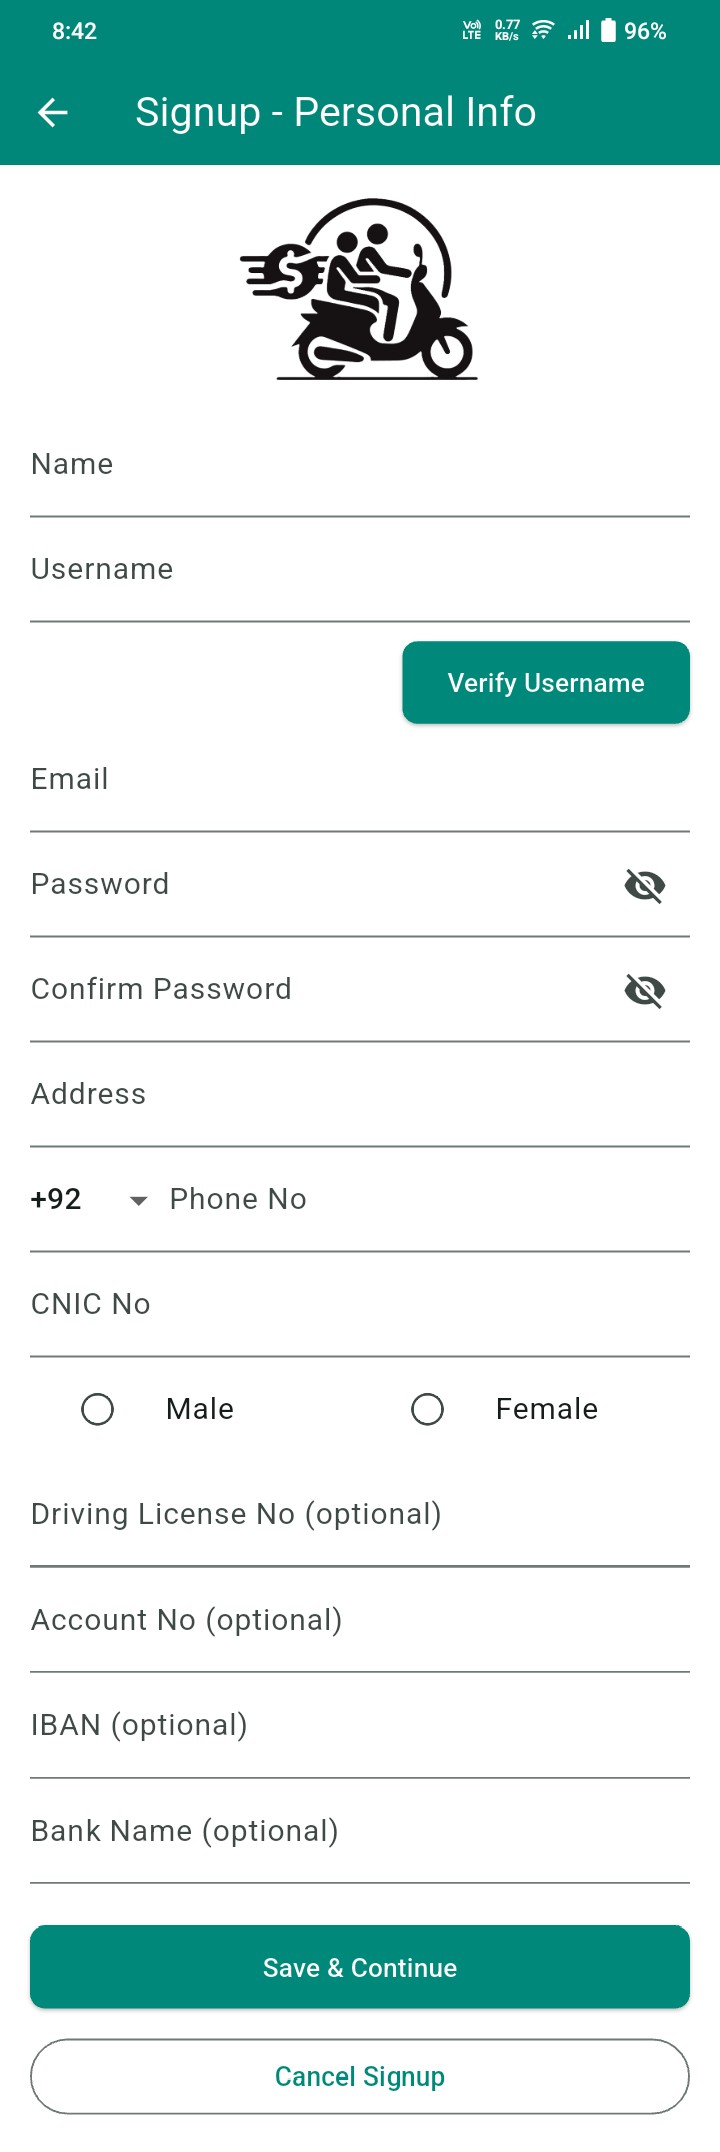
\includegraphics[width=\textwidth,keepaspectratio]{assets/app screenshot/signup_personal_info.jpeg}}
\end{minipage}\hfill
\begin{minipage}{0.23\textwidth}
\centering
\fbox{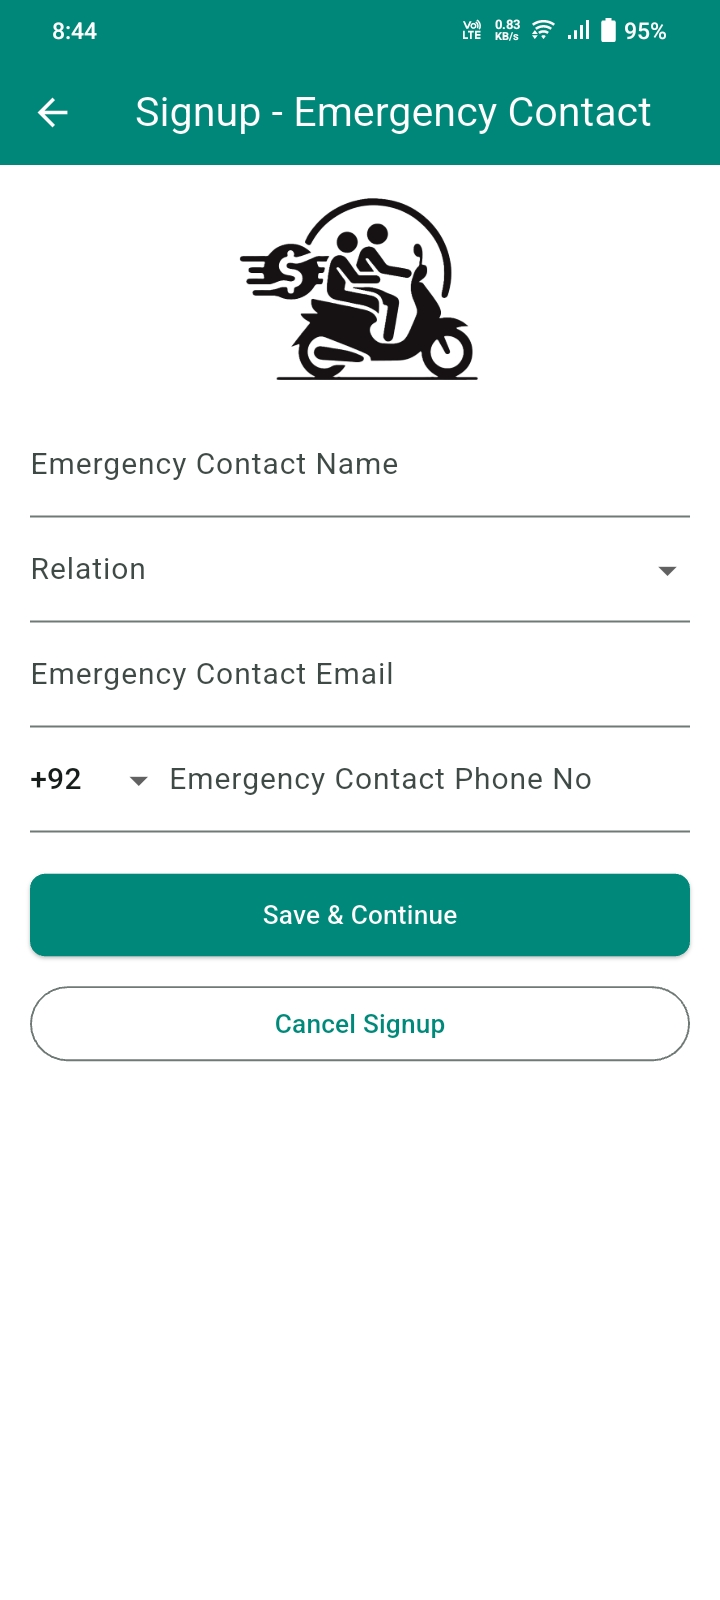
\includegraphics[width=\textwidth,keepaspectratio]{assets/app screenshot/signup_emergency_contact.jpeg}}
\end{minipage}\hfill
\begin{minipage}{0.23\textwidth}
\centering
\fbox{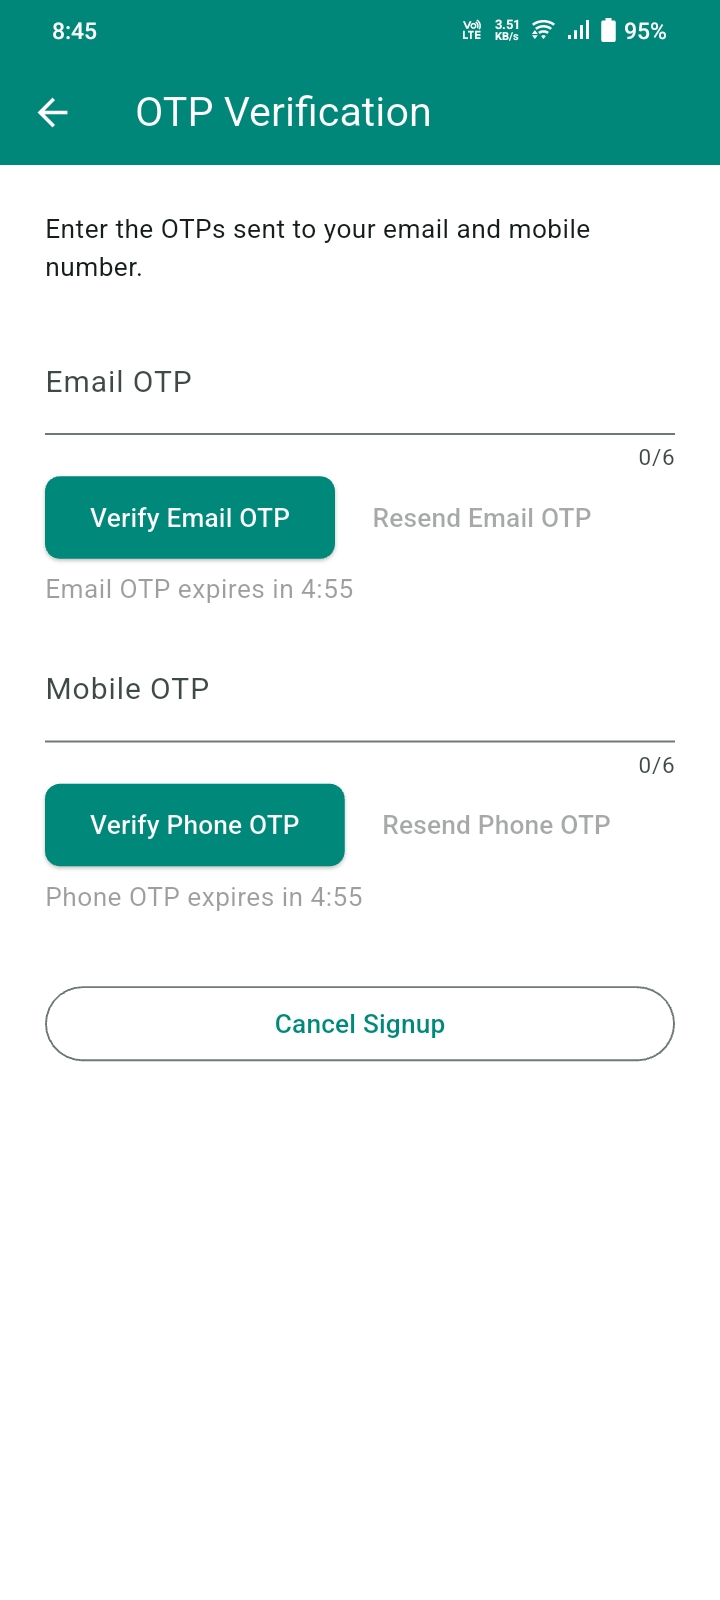
\includegraphics[width=\textwidth,keepaspectratio]{assets/app screenshot/signup_otp_verification.jpeg}}
\end{minipage}\hfill
\begin{minipage}{0.23\textwidth}
\centering
\fbox{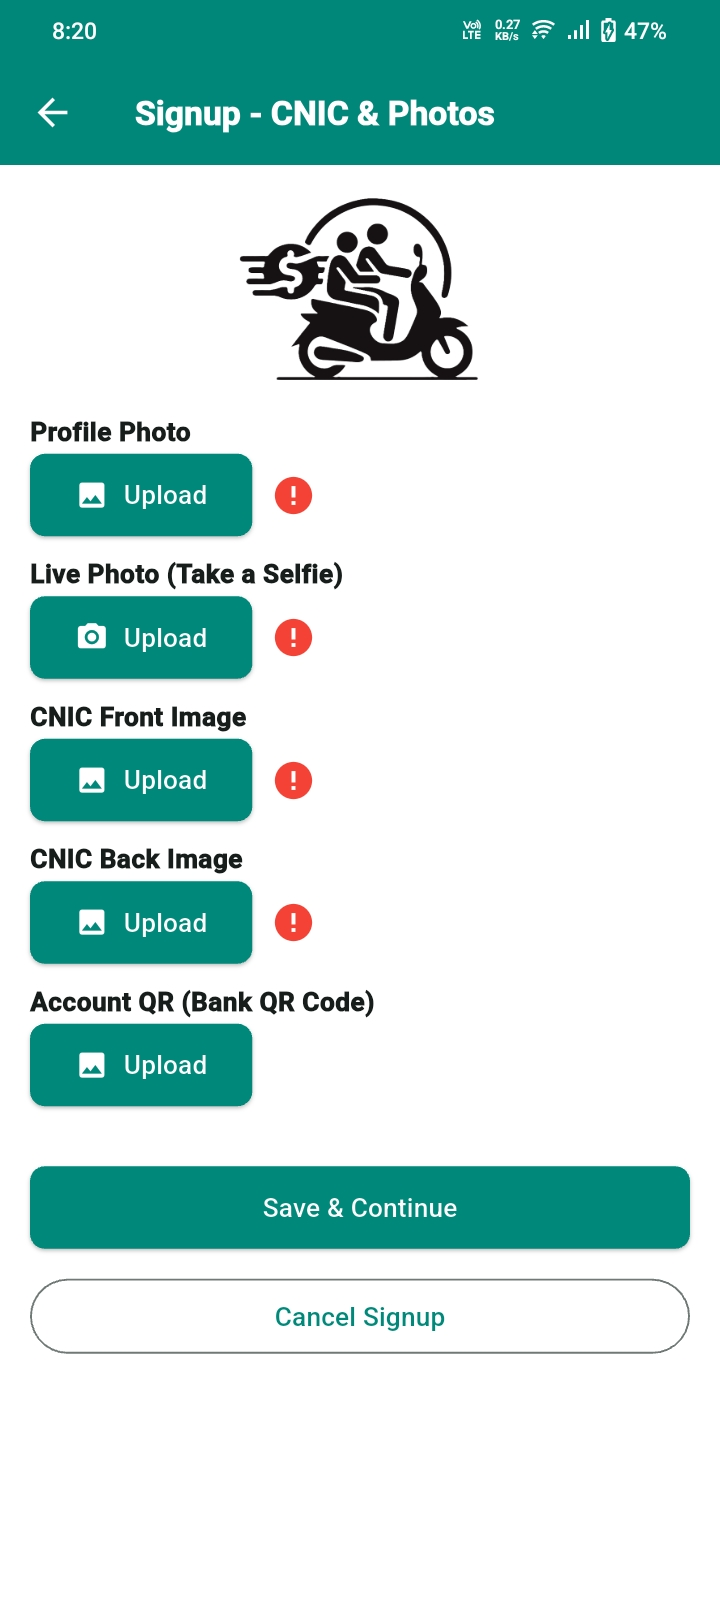
\includegraphics[width=\textwidth,keepaspectratio]{assets/app screenshot/signup_images uploading.jpg}}
\end{minipage}
\caption{User Signup Flow}
\end{figure}

\textbf{Functional Flow:} Enter personal and emergency contact details, upload required images and then complete OTP verification. If the OTP is validated successfully, then the user profile is created and the app moves on to the login/home flow based on the account status.

\textbf{Backend Integration:} Signup endpoints to register users and OTP verification to verify them, user profile data is stored in a backend database.

\textbf{Validation/Security:} Validator for required fields (client side), OTP expiry and retries implemented, validation for uploaded images implemented before submission.

\subsubsection{Screen 4: Login Screen}

\textbf{Function:} Where current users come from to use the platform.

\textbf{Components:}
\begin{itemize}
    \item Textboxes for text and password input.
    \item Remember Me checkbox.
    \item Type ``Login'' button and navigation to registration and forgot password flows.
\end{itemize}

\begin{figure}[H]
\centering
\fbox{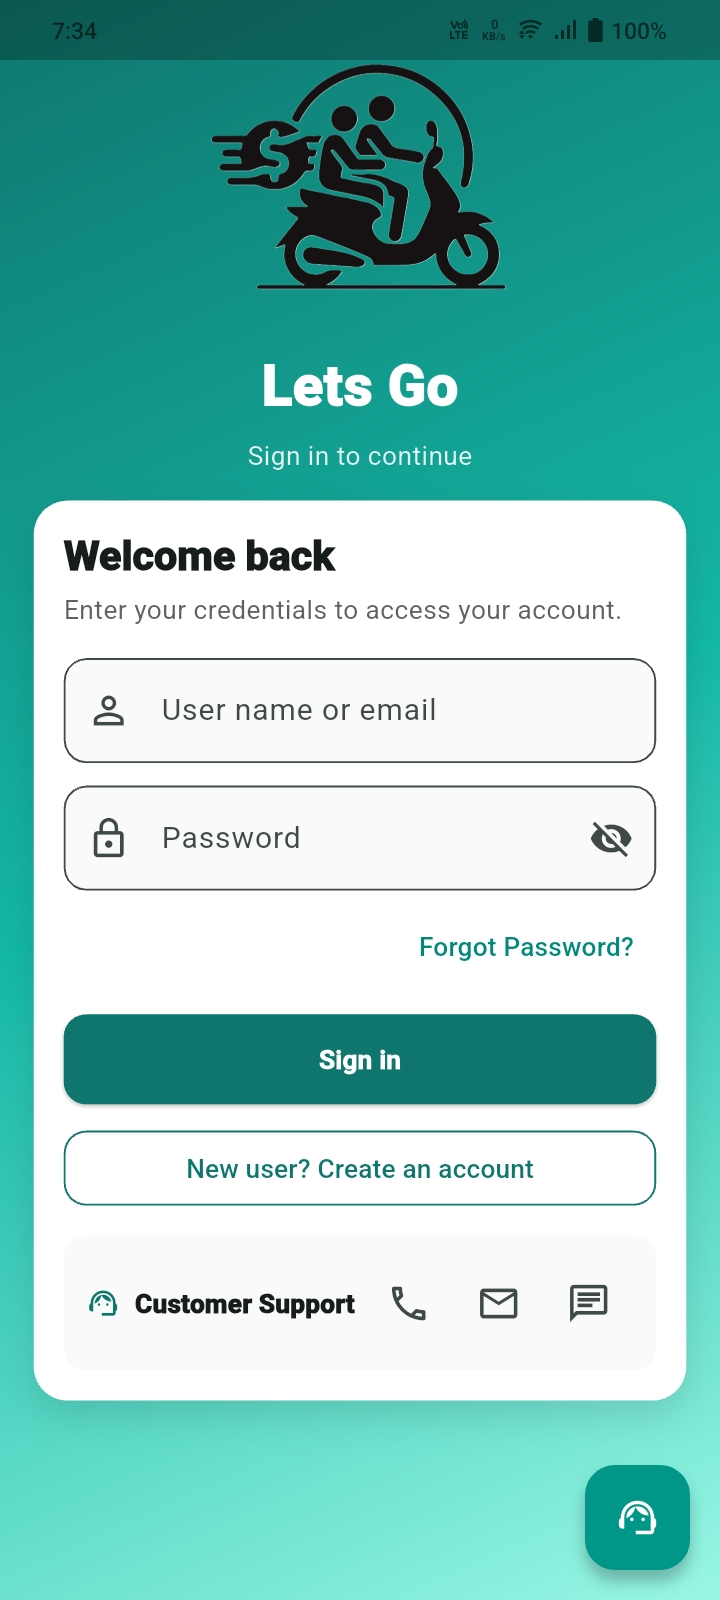
\includegraphics[width=0.45\textwidth,keepaspectratio,height=0.8\textheight]{assets/app screenshot/login_screen.jpeg}}
\caption{Login Screen}
\end{figure}

\textbf{Functional Flow:} The user enters the login information and clicks on the login form. A session is created and the user is taken to Home / Dashboard page if authentication is successful.

\textbf{Backend Integration:} The screen requests authentication credentials from the security end point to verify them and then requests the user profile payload to be used for navigation.

\textbf{Validation/Security:} Fields are blanked, error messages are provided if the credentials are invalid, and authentication calls are passed with session-based authorization.

\subsubsection{Screen 5: Account Status (Banned/Rejected)}

A screen displaying Account Status (Banned/Rejected).A screen that shows if the account is banned or rejected.

\textbf{Instructions:} If access is denied by Admin review, this will let the user know.

\textbf{Components:}
\begin{itemize}
    \item Status illustration and clear warning message.
    \item Contact Support option for appealing the decision.
\end{itemize}

\begin{figure}[H]
\centering
\begin{minipage}{0.30\textwidth}
\centering
\fbox{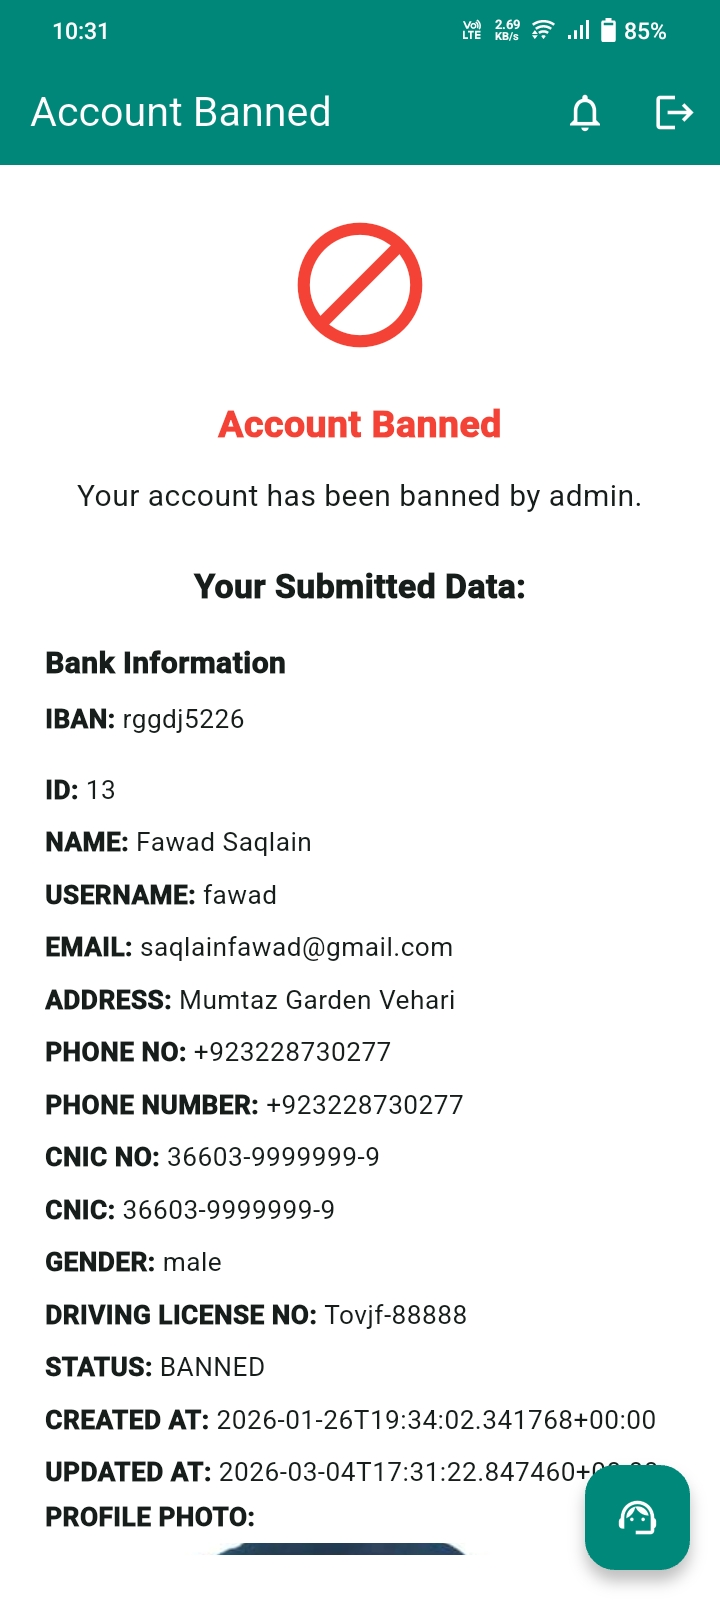
\includegraphics[width=\textwidth,keepaspectratio]{assets/app screenshot/account_banned.jpeg}}
\end{minipage}\hfill
\begin{minipage}{0.30\textwidth}
\centering
\fbox{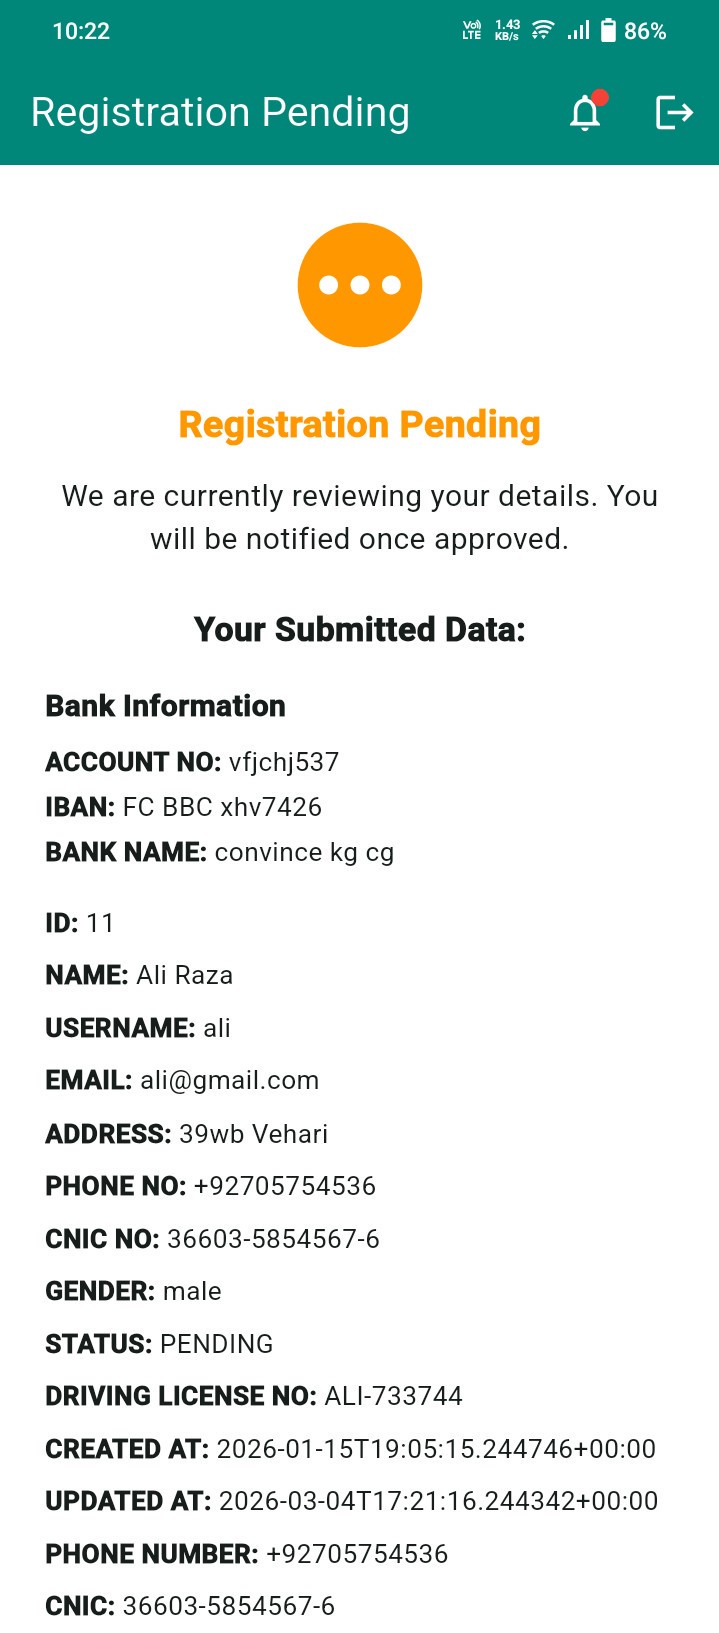
\includegraphics[width=\textwidth,keepaspectratio]{assets/app screenshot/account_pending.jpeg}}
\end{minipage}\hfill
\begin{minipage}{0.30\textwidth}
\centering
\fbox{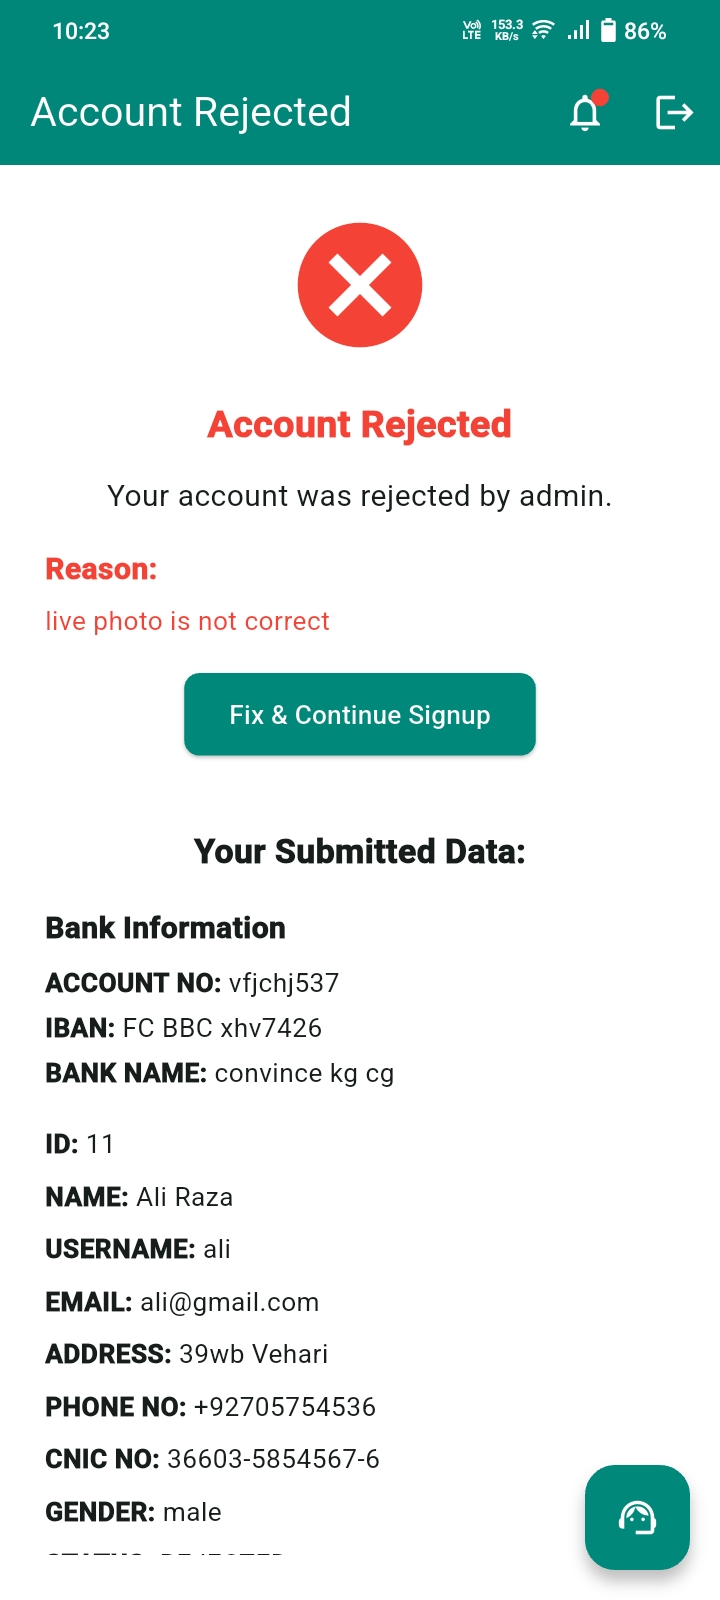
\includegraphics[width=\textwidth,keepaspectratio]{assets/app screenshot/account_rejected.jpeg}}
\end{minipage}
\caption{Account Status (Banned/Rejected)}
\end{figure}

\textbf{Login/signup and account status check:} This is a functional flow where after login/signup, the app validates the account status. When the account is pending, banned or rejected, the user is presented with a clear status screen with instructions and a support link.

\textbf{Backend Integration:} Status is taken from the user profile response and/or a status check endpoint.

\textbf{Server-side account gating:} Access to gated flows is denied if the user is not approved.

\subsubsection{Create Ride: Simplified Posting Flow}

\textbf{Purpose:} A driver ride posting simplified process from route selection to ride confirmation.

\begin{figure}[H]
\centering
\begin{minipage}{0.30\textwidth}
\centering
\fbox{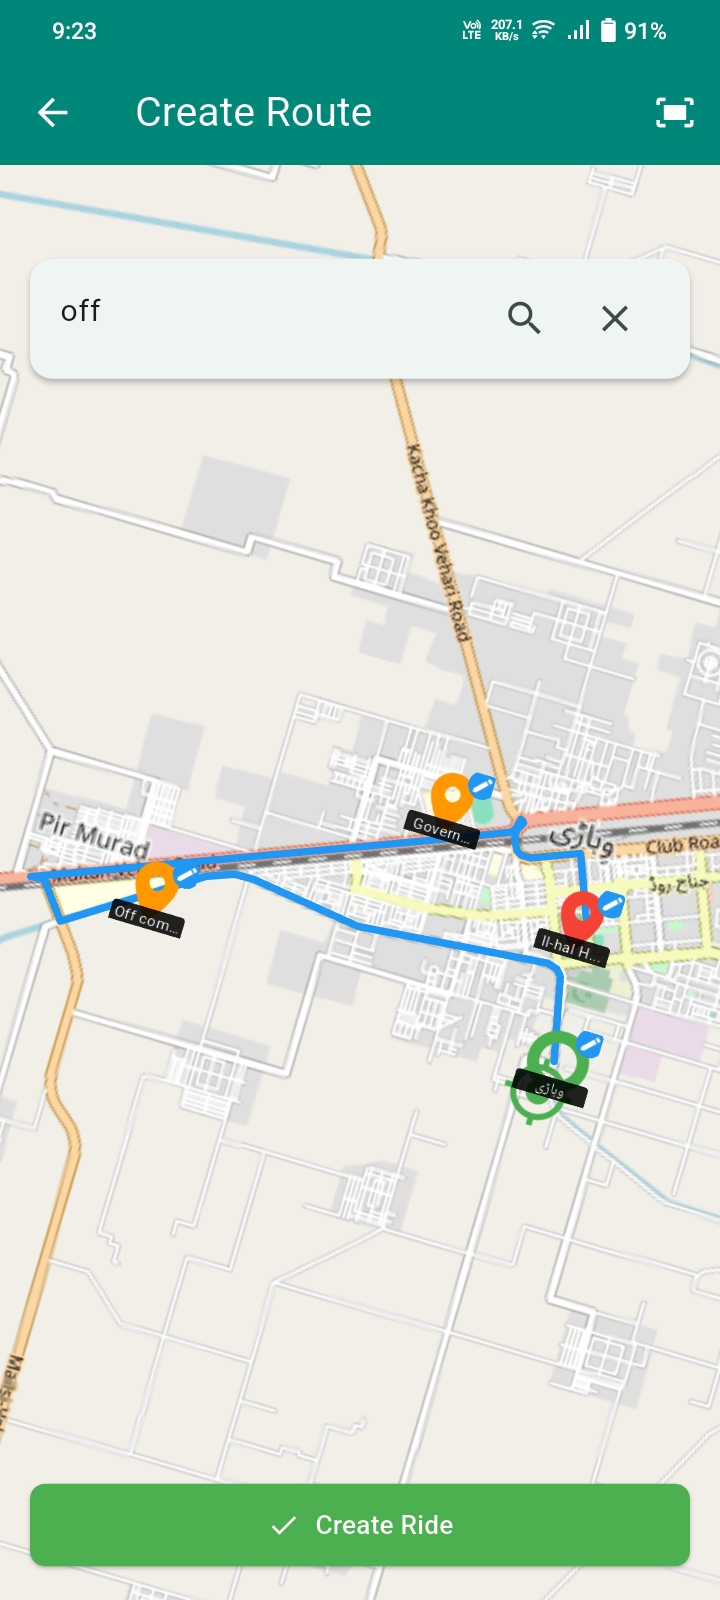
\includegraphics[width=\textwidth,keepaspectratio]{assets/app screenshot/create_route_map_view.jpeg}}
\end{minipage}\hfill
\begin{minipage}{0.30\textwidth}
\centering
\fbox{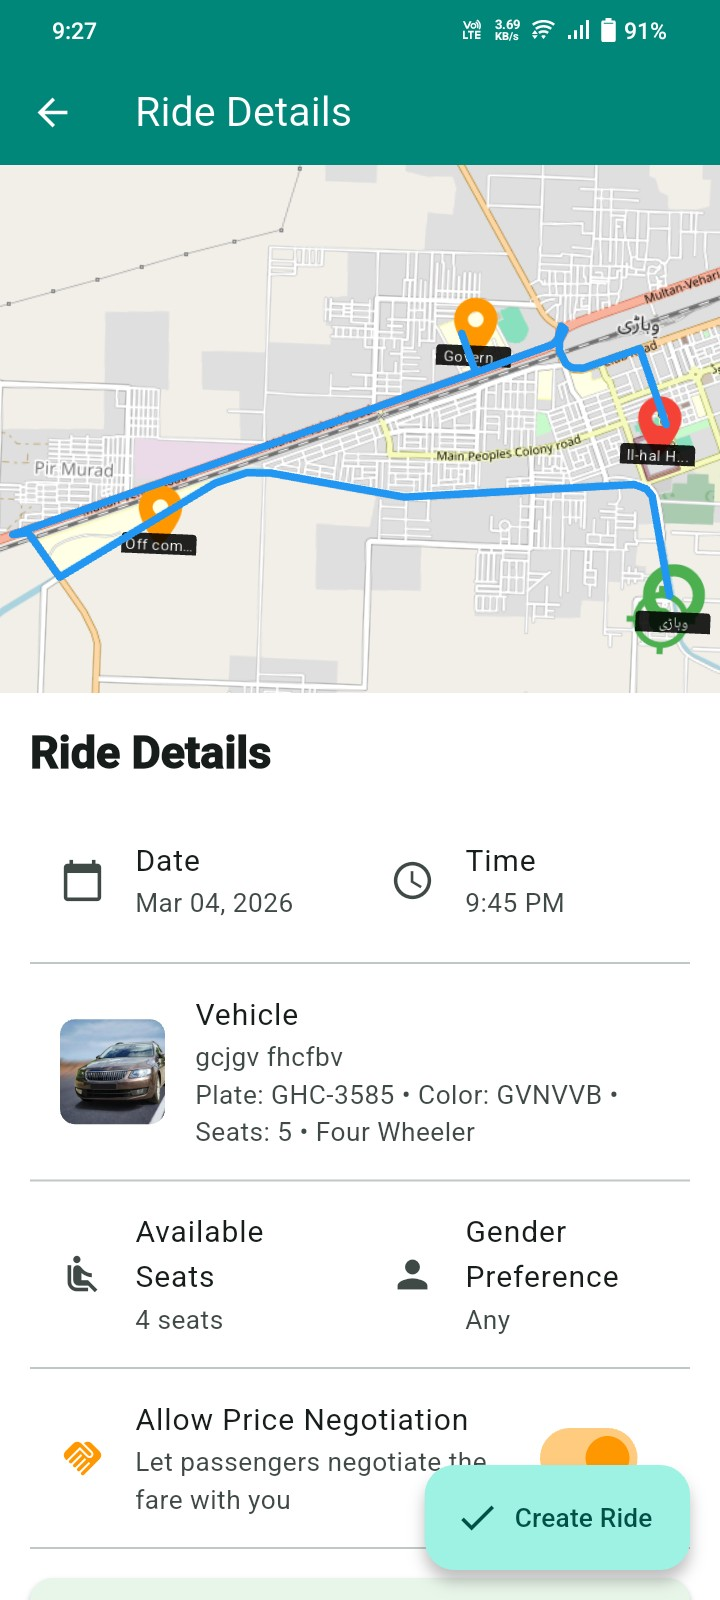
\includegraphics[width=\textwidth,keepaspectratio]{assets/app screenshot/create_ride_summary.jpeg}}
\end{minipage}\hfill
\begin{minipage}{0.30\textwidth}
\centering
\fbox{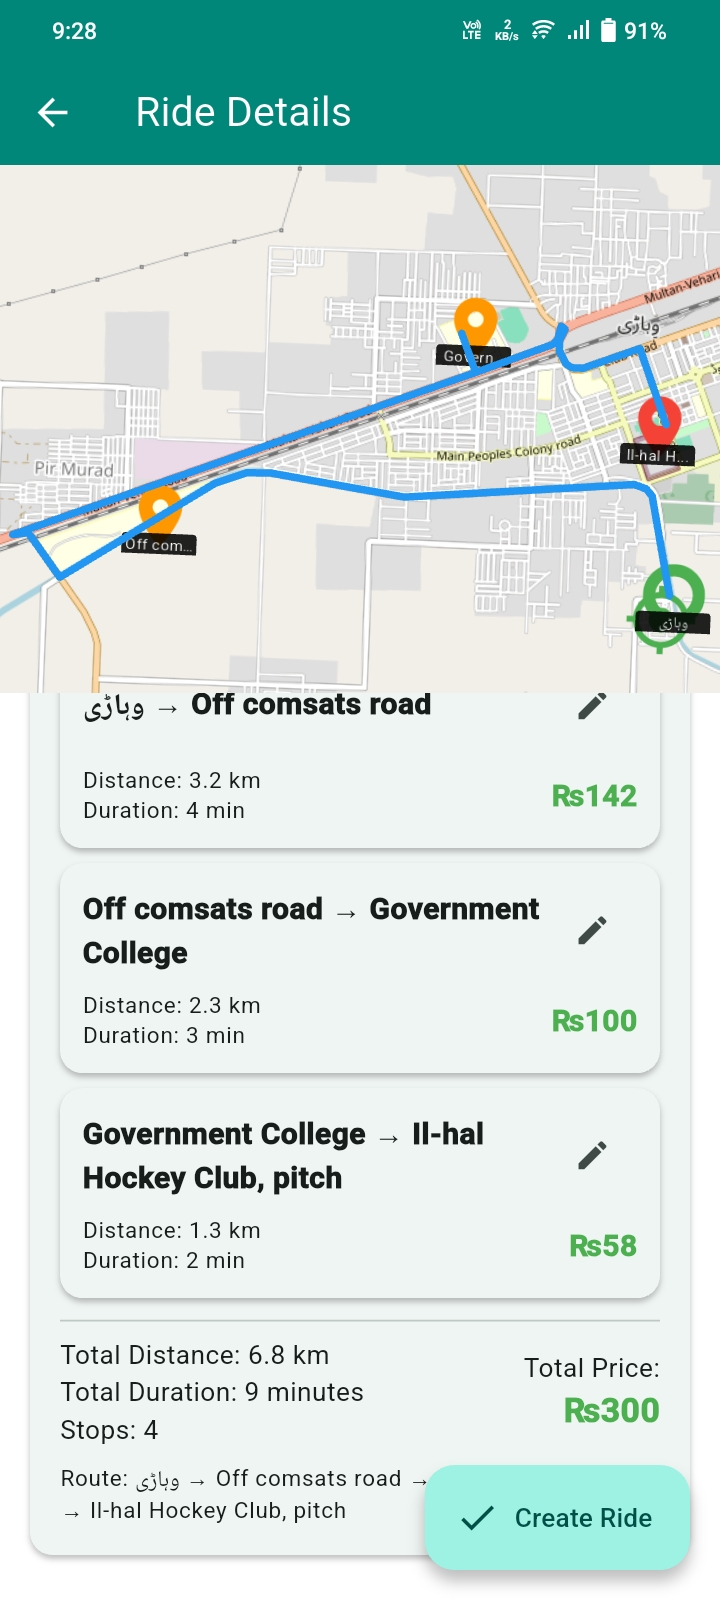
\includegraphics[width=\textwidth,keepaspectratio]{assets/app screenshot/create_ride_final_details.jpeg}}
\end{minipage}
\caption{Create Ride Posting Flow (Map View, Summary, and Final Details)}
\end{figure}

\textbf{Functional Flow:} Driver enters a route on the map, looks at a ridesummary and clears the final ride data and publishes the ride. Once the ride is submitted, it will appear in the passenger search results.

\textbf{Backend integration:} Flow calls ride creation endpoints and stores route geometries, stops, seats, and fare settings in the backend.

\textbf{Validation/Security:} Input constraints (seats, time, fare) are checked for validation and only validly authenticated drivers with valid profiles can post rides.

\subsubsection{Screen 14-16: Find Ride (Browse, Pickup/Drop, and Filters)}

\textbf{Goal:} User wants to see the available rides, choose which one to pickup/drop and filter the results.

\textbf{Components:}
\begin{itemize}
    \item Home and Work location search boxes.
    \item Visual location markers.
    \item Pickup/drop selection and ride filtering.
\end{itemize}

\begin{figure}[H]
\centering
\begin{minipage}{0.30\textwidth}
\centering
\fbox{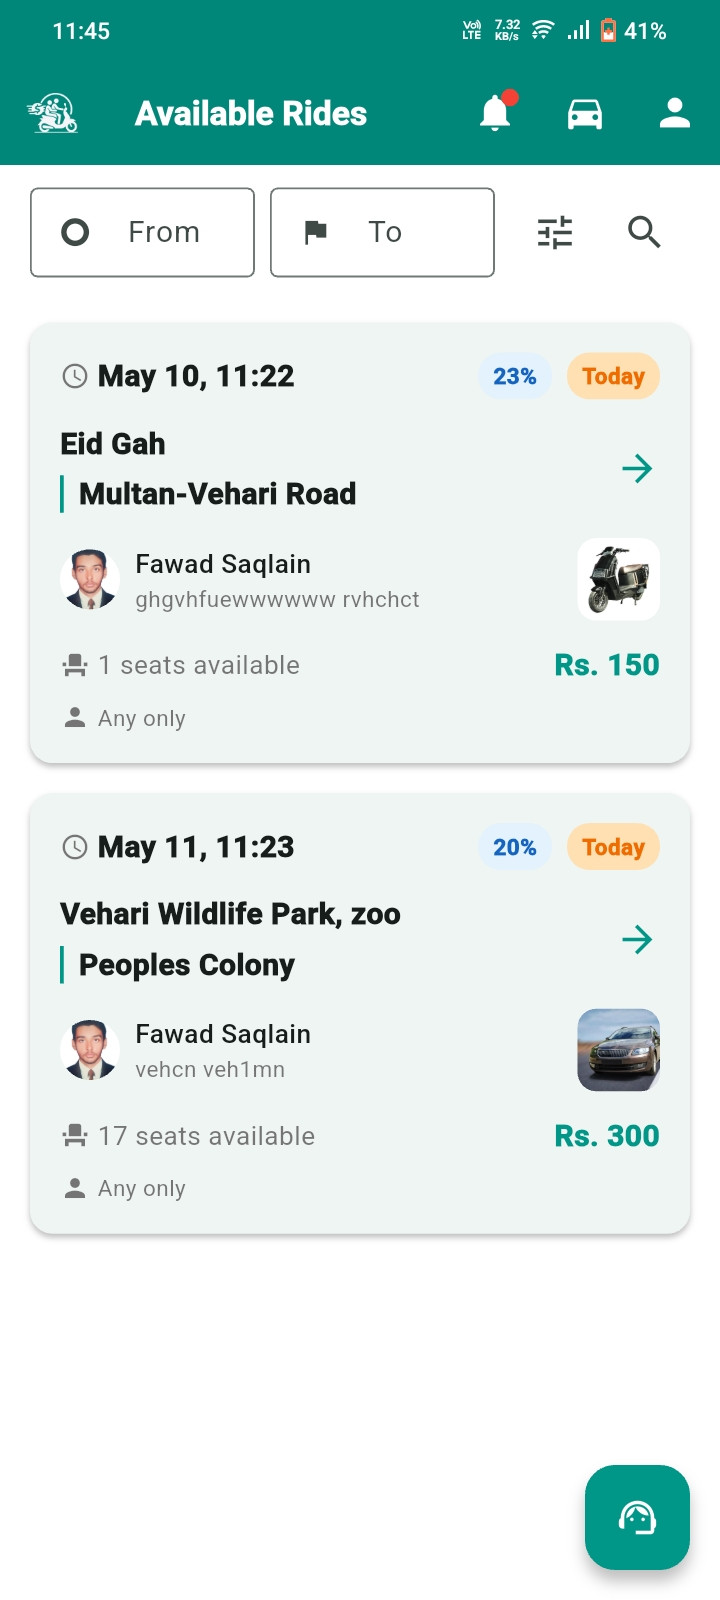
\includegraphics[width=\textwidth,keepaspectratio]{assets/app screenshot/find_ride_available_rides.jpeg}}
\end{minipage}\hfill
\begin{minipage}{0.30\textwidth}
\centering
\fbox{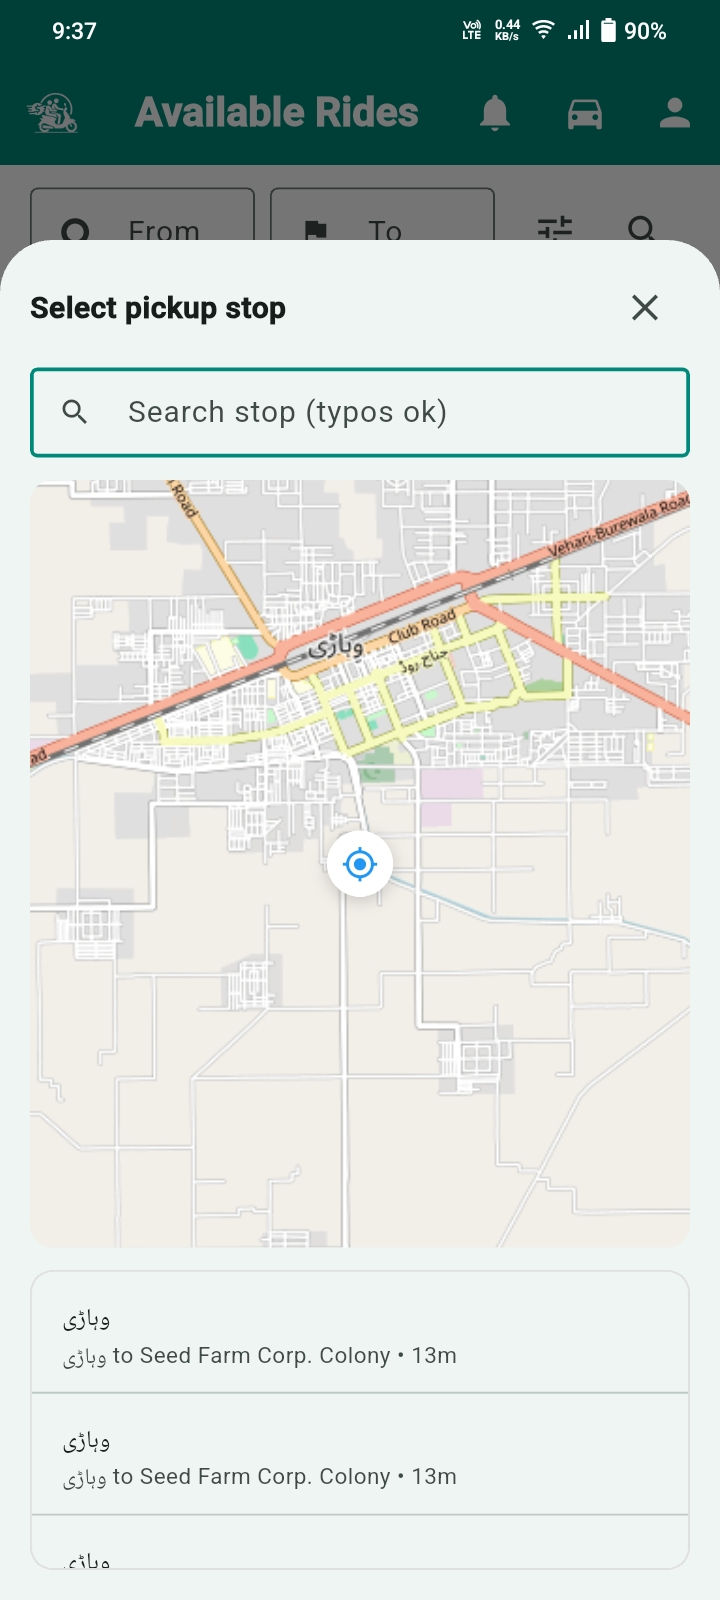
\includegraphics[width=\textwidth,keepaspectratio]{assets/app screenshot/find_ride_select_pickup.jpeg}}
\end{minipage}\hfill
\begin{minipage}{0.30\textwidth}
\centering
\fbox{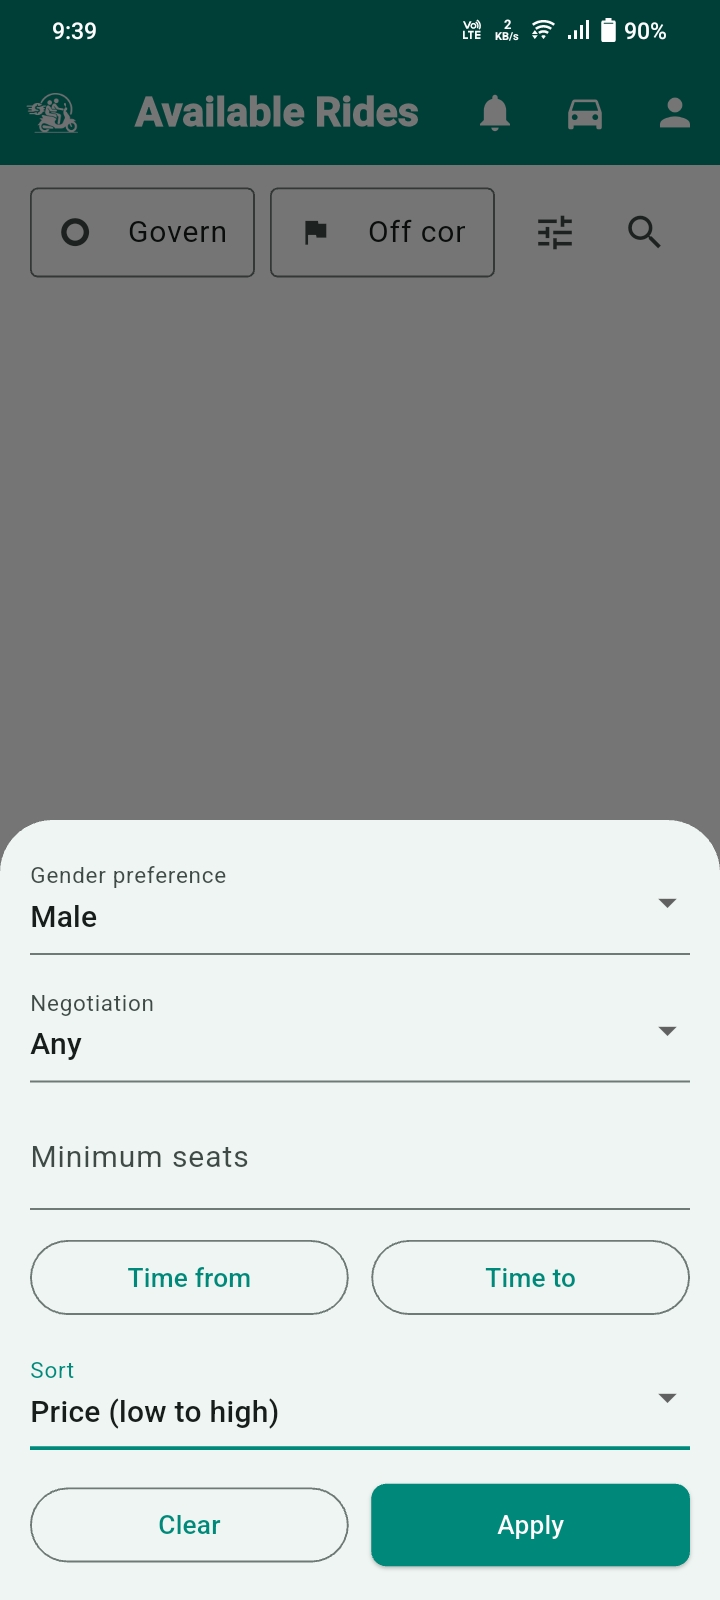
\includegraphics[width=\textwidth,keepaspectratio]{assets/app screenshot/find_ride_filters.jpeg}}
\end{minipage}
\caption{Find Ride Flow (Available Rides, Pickup/Drop, and Filters)}
\end{figure}

\textbf{Functional Flow:} The Functional Flow is pretty easy to use: Users review a list of rides, choose a pickup location, choose a drop location, and use a filter to narrow their choices. Clicking on ``Select a ride'' will switch to the Ride Details view.

\textbf{Backend Integration:} Search Endpoints: The list and filters are driven by trip search end points which include query parameters like route, time window and seat availability.

\textbf{Validation/Security:} Filters are sanitized and results are limited to the current user session and platform rules.

\subsubsection{Screen 17: Ride Details View}

The Ride Details View is the next screen.The next screen is the Ride Details View.

\textbf{Aim:} All ride parameters for passenger review detailed.

\textbf{Components:}
\begin{itemize}
    \item Driver profile, vehicle information and trip timeline.
\end{itemize}

\begin{figure}[H]
\centering
\begin{minipage}{0.45\textwidth}
\centering
\fbox{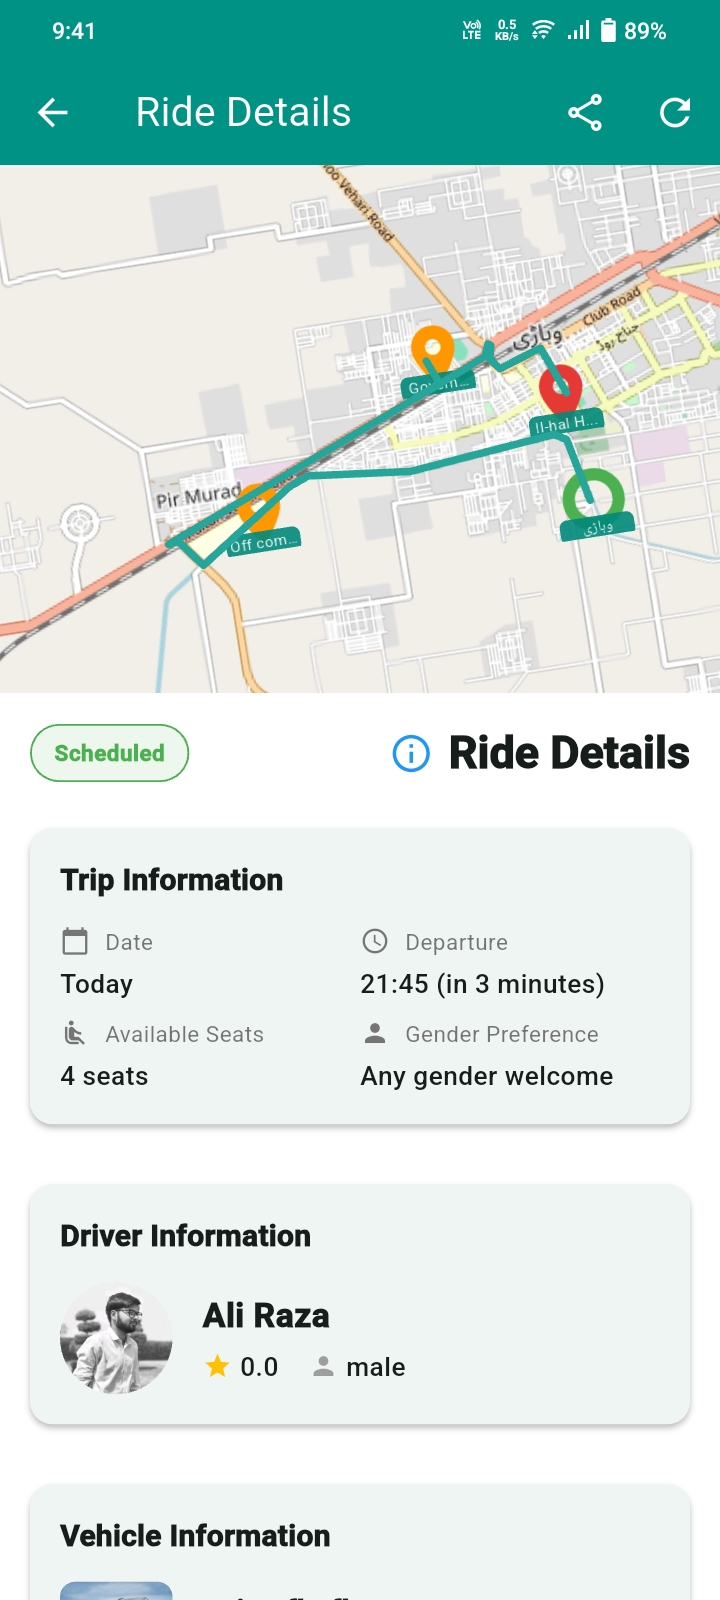
\includegraphics[width=\textwidth,keepaspectratio]{assets/app screenshot/ride_details part 1.jpeg}}
\end{minipage}\hfill
\begin{minipage}{0.45\textwidth}
\centering
\fbox{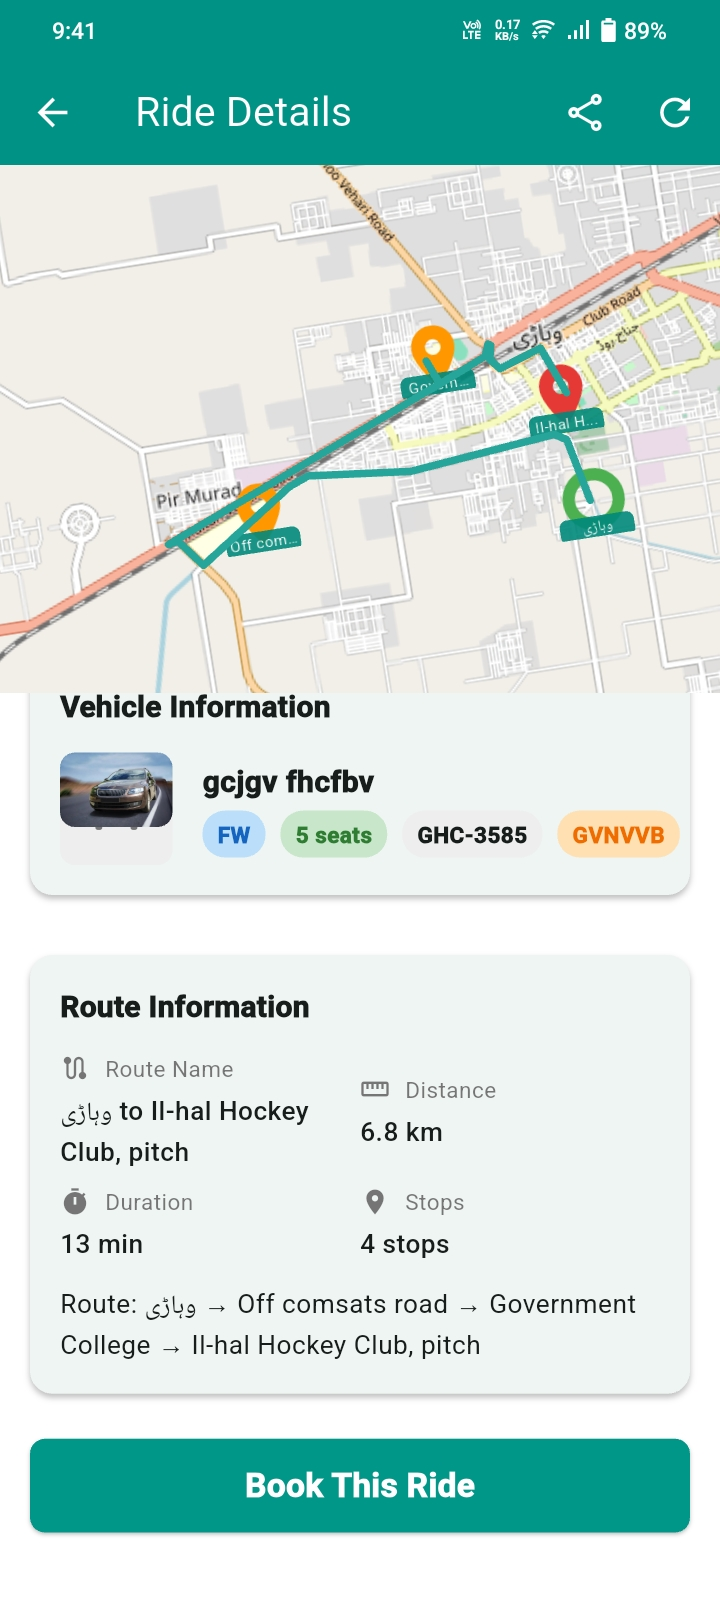
\includegraphics[width=\textwidth,keepaspectratio]{assets/app screenshot/ride_details part 2.jpeg}}
\end{minipage}
\caption{Ride Details View}
\end{figure}

\textbf{Functional Flow:} The passenger reads the driver and ride information (route and time) and then goes to the booking/request screen. This screen is used to confirm a booking prior to making a booking.

\textbf{Backend Integration:} Rides are retrieved from the backend using the trip identifier and will contain data like driver profile and stops.

\textbf{Validation/Security:} The UI hides actions if the ride is unavailable and blocks booking without valid session context.

\subsubsection{Screen 18: Request Ride (Booking Form)}

\textbf{Use case:} Enables passengers to view the route overview and to submit a ride request with seat selection, optional price negotiation and special notes.

\textbf{Components:}
\begin{itemize}
    \item An overview map and trip report (date, time, length of trip, cost of trip).
    \item Negotiation input, seat selection, and gender selection in pick-up/drop-off.
\end{itemize}

\begin{figure}[H]
\centering
\begin{minipage}{0.40\textwidth}
\centering
\fbox{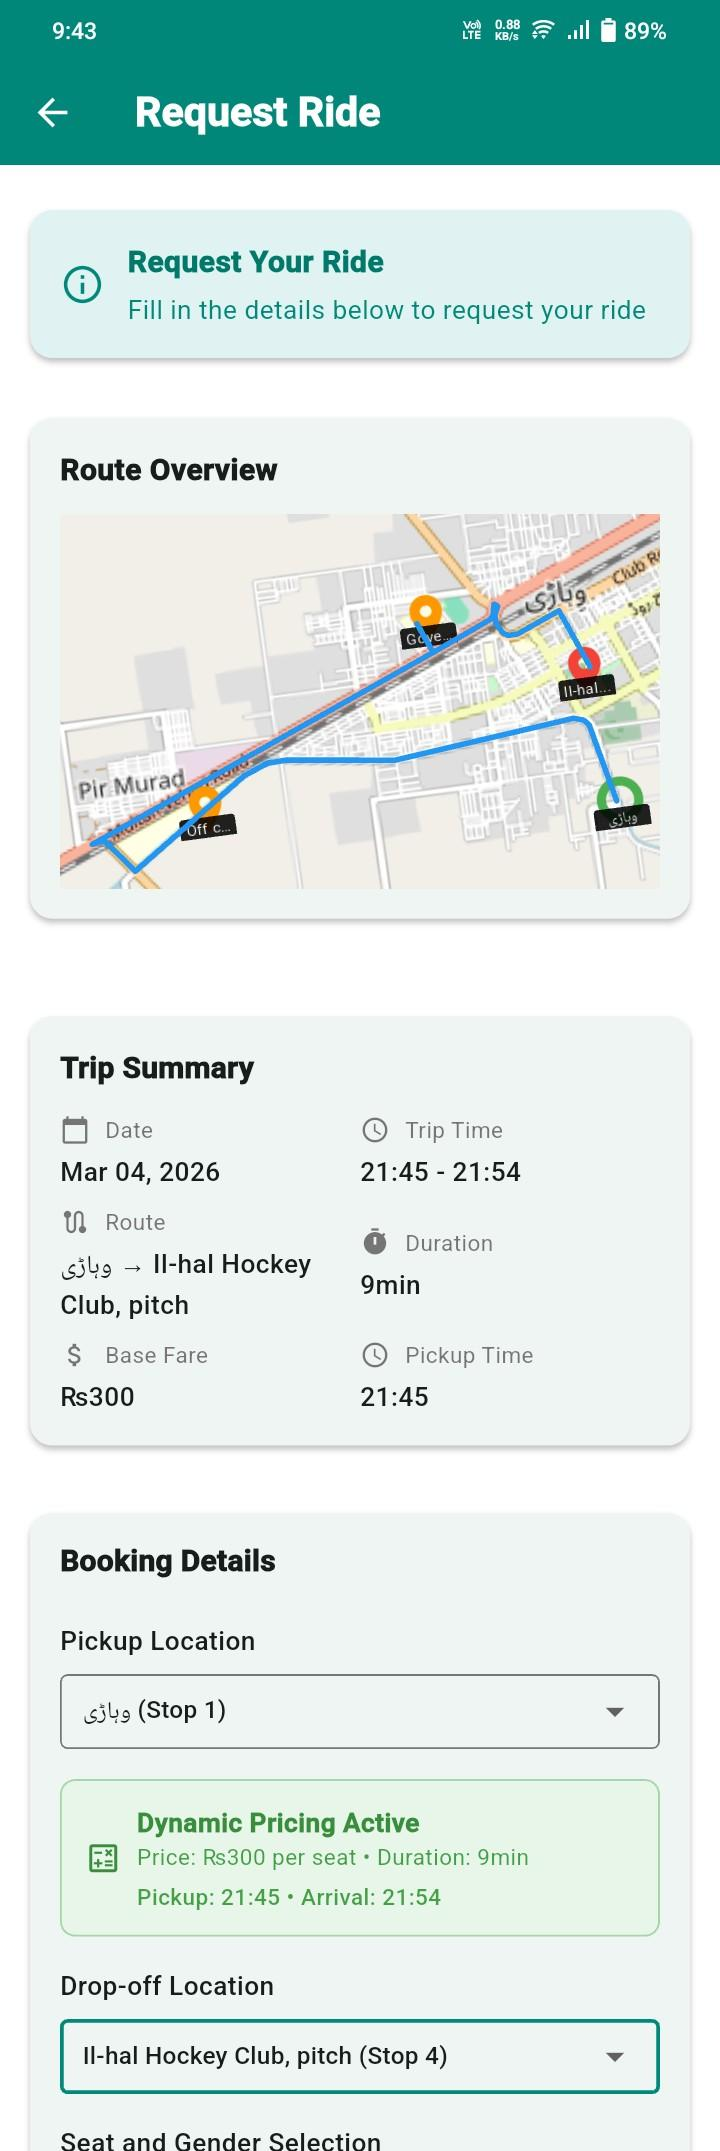
\includegraphics[width=\textwidth,height=0.72\textheight,keepaspectratio]{assets/app screenshot/ride_request_part1.jpeg}}
\end{minipage}\hfill
\begin{minipage}{0.40\textwidth}
\centering
\fbox{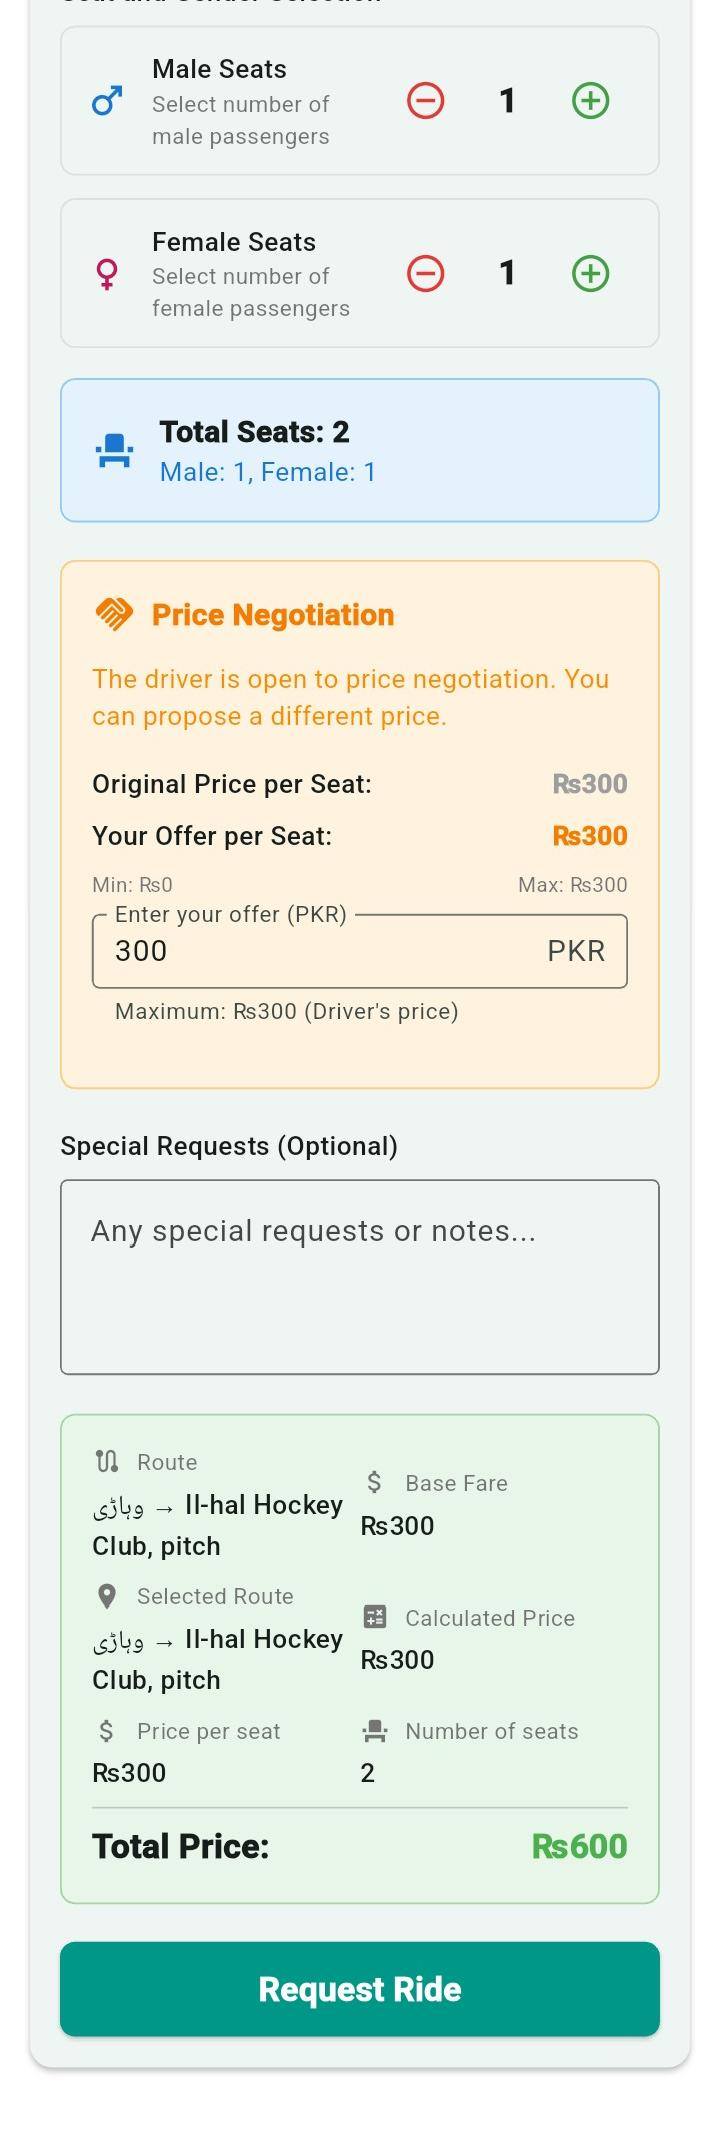
\includegraphics[width=\textwidth,height=0.72\textheight,keepaspectratio]{assets/app screenshot/ride_request_part2.jpeg}}
\end{minipage}
\caption{Request Ride (Booking Form)}
\end{figure}

\textbf{Functional Flow:} Passenger chooses pickup/drop stops and seats, optionally offers counter fare, submits request. The request will then be in a pending/negotiation state until the driver responds.

\textbf{Backend Integration:} Sends a booking request payload which is associated with the trip and passenger profile and sends notifications for driver review.

\textbf{Validation/Security:} If more people than seats are available, the reservation is not processed and if a wrong stop is selected, it is rejected.

\subsubsection{Screen 19: Booked Ride Details}

\textbf{Aim:} Choosing seats and confirming booking conditions.

\textbf{Components:}
\begin{itemize}
    \item Number of seats available, and certain seating choices.
\end{itemize}

\begin{figure}[H]
\centering
\begin{minipage}{0.45\textwidth}
\centering
\fbox{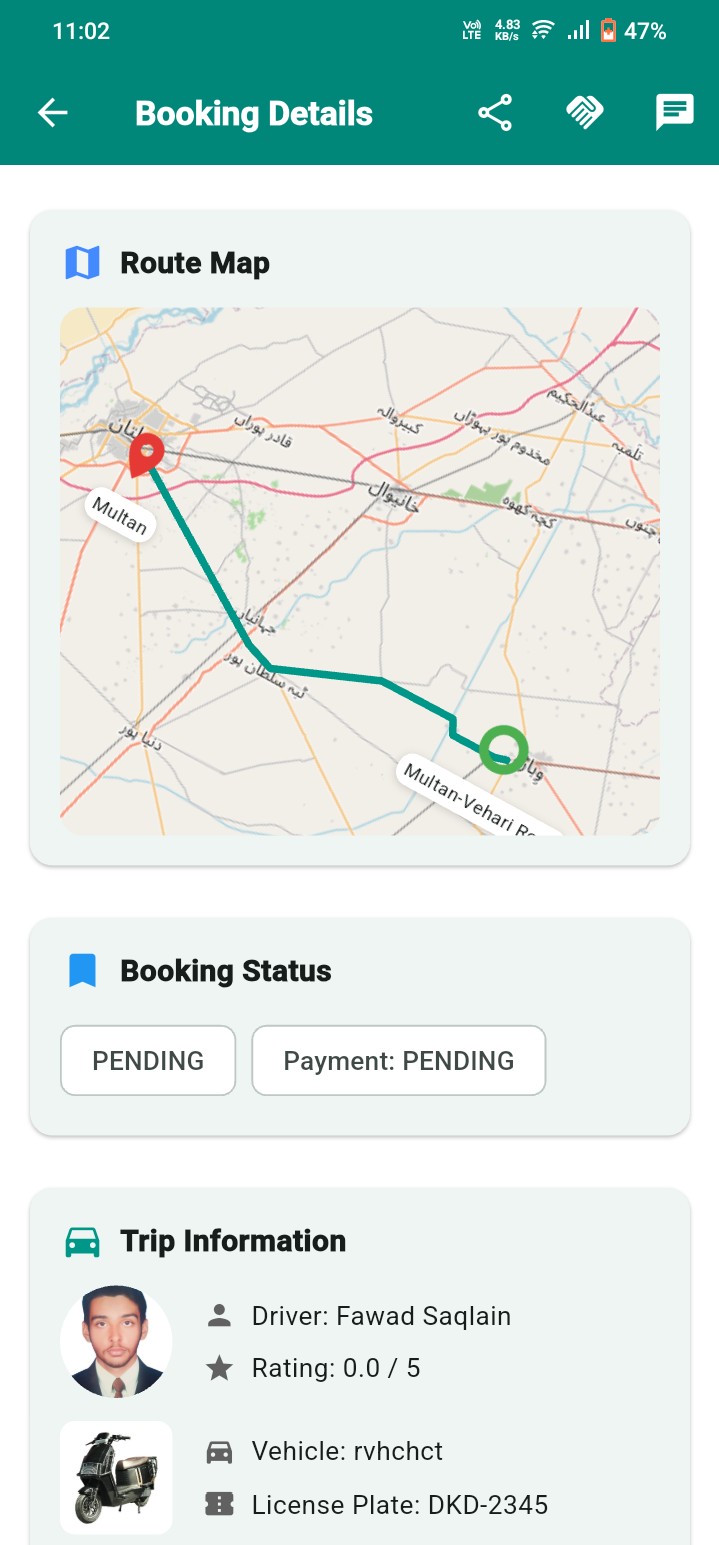
\includegraphics[width=\textwidth,height=0.42\textheight,keepaspectratio]{assets/app screenshot/passenger_booking_details_pending part 1.jpeg}}
\end{minipage}\hfill
\begin{minipage}{0.45\textwidth}
\centering
\fbox{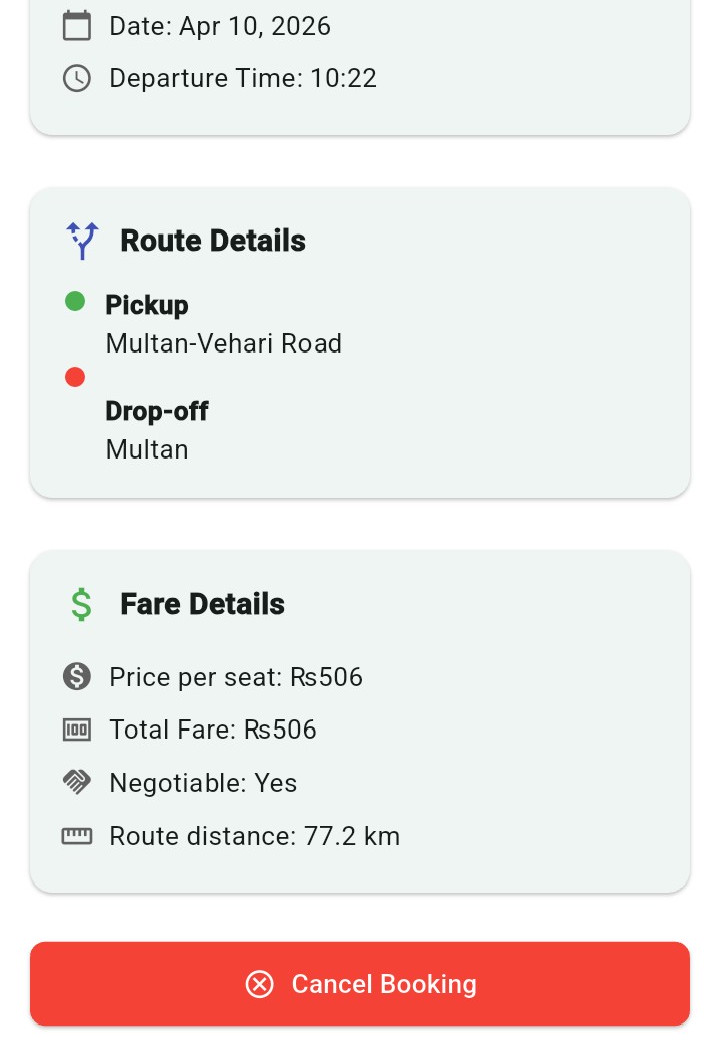
\includegraphics[width=\textwidth,keepaspectratio]{assets/app screenshot/passenger_booking_details_pending part 2.jpeg}}
\end{minipage}
\caption{Booked Ride Details}
\end{figure}

\textbf{Functional Flow:} After the booking is completed, the passenger sees the booking details and the seat allocation state. The screen is updated as the driver accepts, rejects or negotiates with the updates.

\textbf{Backend Integration:} loads booking information from the bookings endpoints and will periodically refresh for state changes.

\textbf{Validation/Security:} Only the owner of the booking is able to see the details and sensitive fields are limited by role.

\subsubsection{Screen 21: Negotiation Between Passenger and Driver}

This can be used when negotiating the price when booking, where both the driver and passenger can view and comment on the negotiation.

\textbf{Components:}
\begin{itemize}
    \item Information about negotiations and counter offers.
    \item Response controls and request status update.
\end{itemize}

\begin{figure}[H]
\centering
\begin{minipage}{0.30\textwidth}
\centering
\fbox{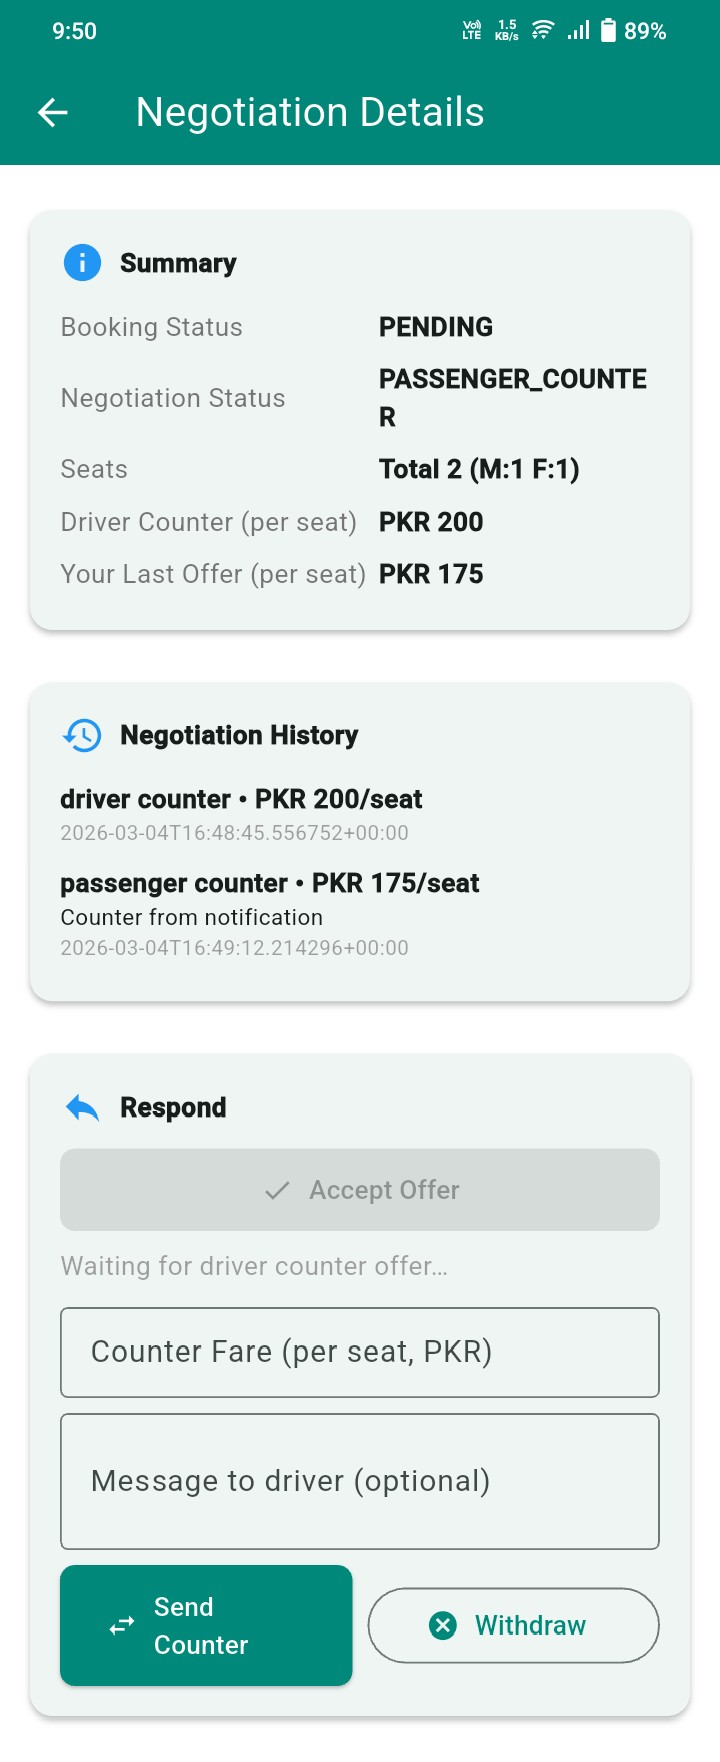
\includegraphics[width=\textwidth,keepaspectratio]{assets/app screenshot/passenger_negotiation_details.jpeg}}
\end{minipage}\hfill
\begin{minipage}{0.30\textwidth}
\centering
\fbox{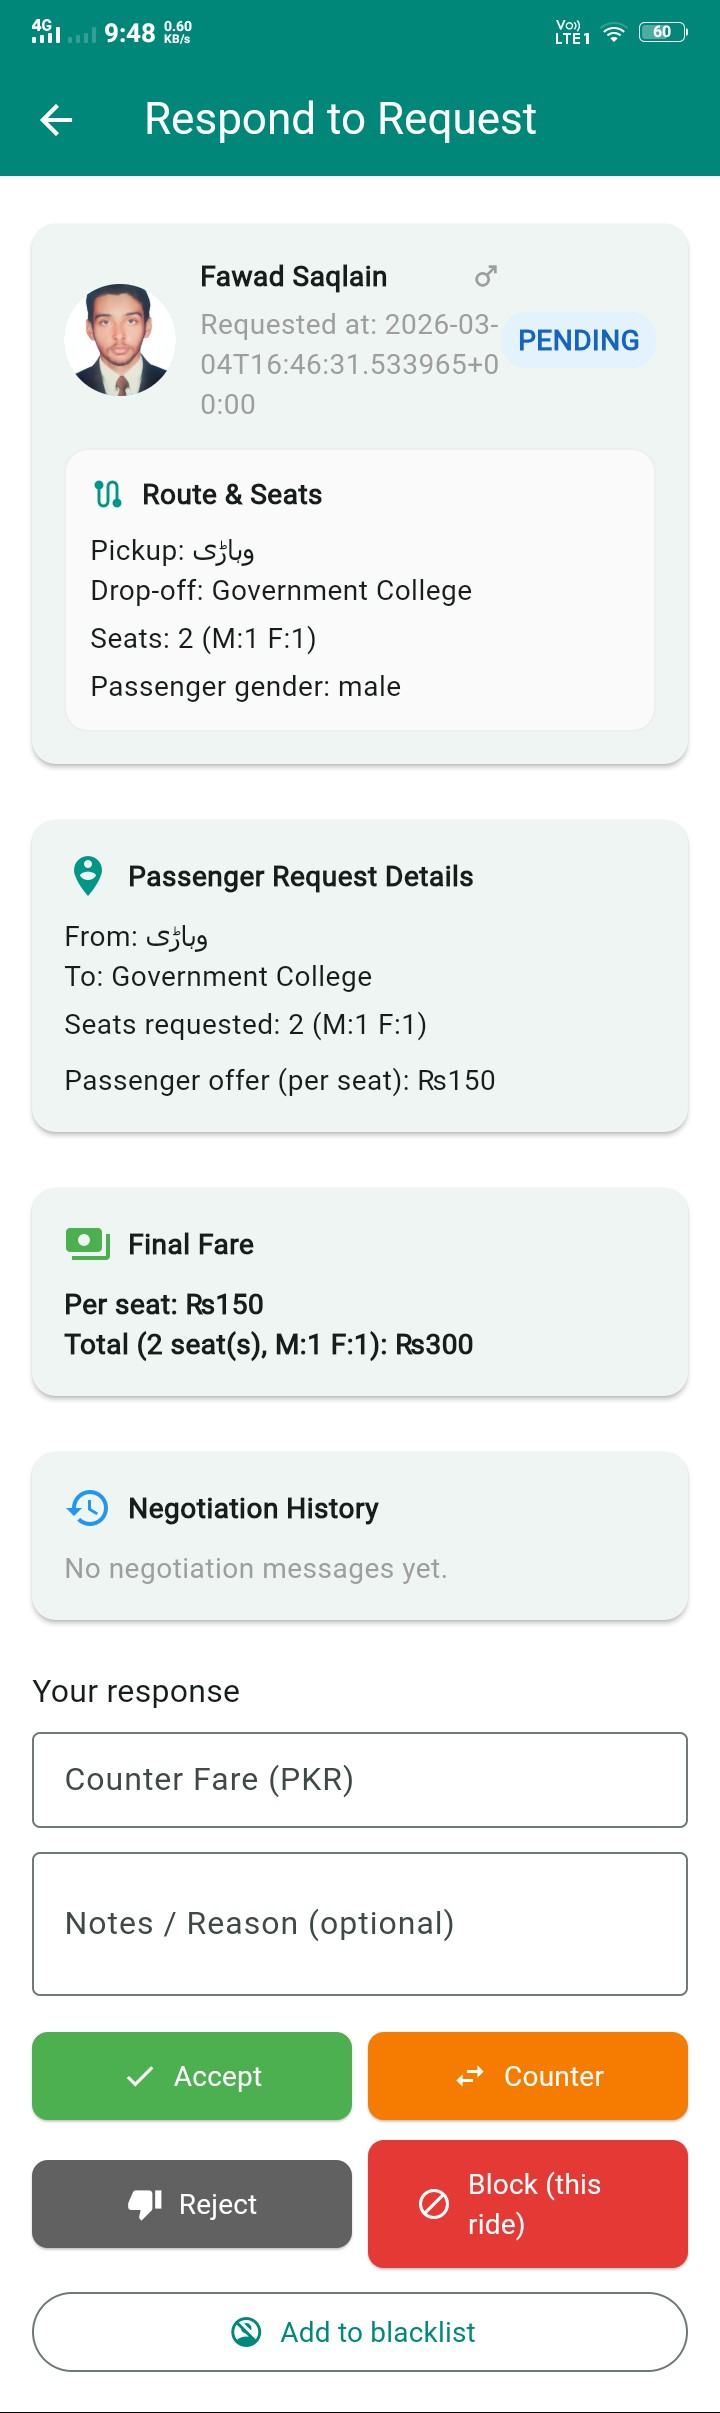
\includegraphics[width=\textwidth,keepaspectratio]{assets/app screenshot/driver_response_screen.jpeg}}
\end{minipage}\hfill
\begin{minipage}{0.30\textwidth}
\centering
\fbox{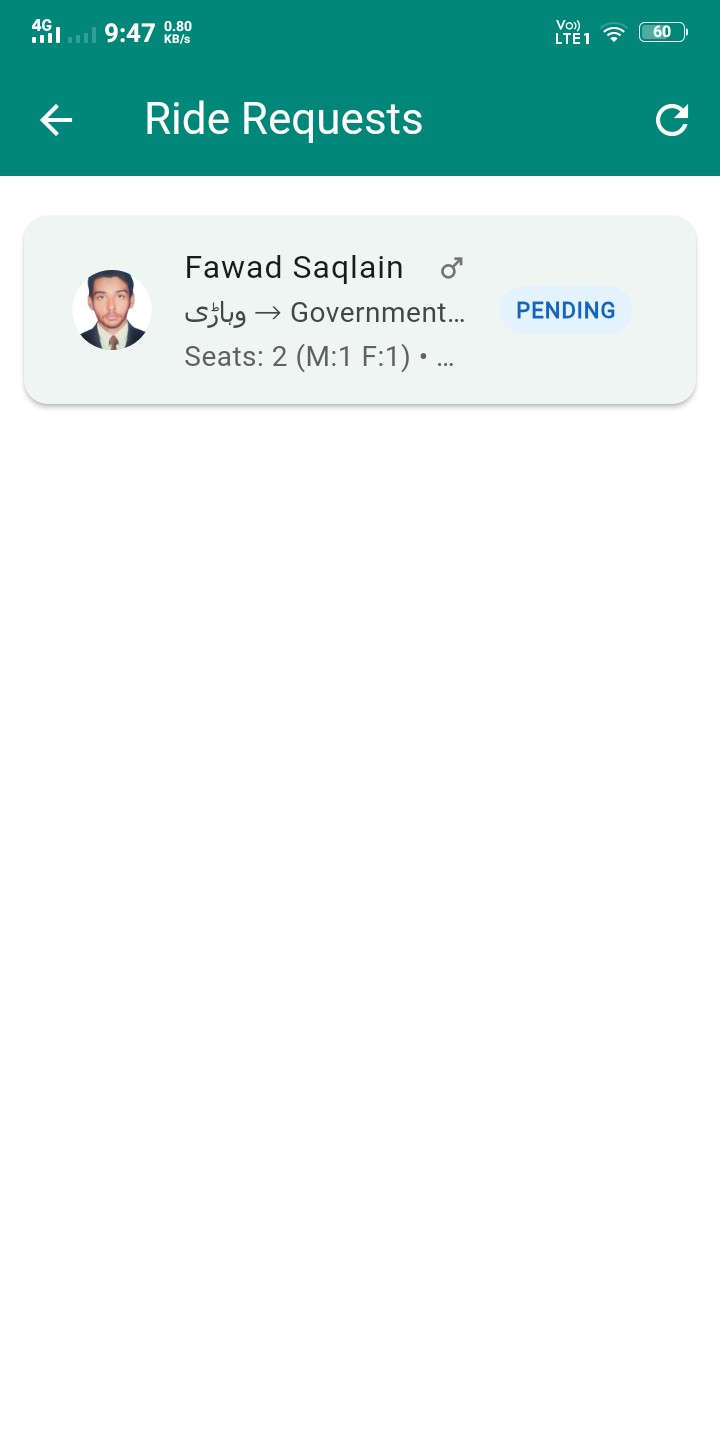
\includegraphics[width=\textwidth,keepaspectratio]{assets/app screenshot/driver_ride_requests_pending.jpeg}}
\end{minipage}
\caption{Negotiation Between Passenger and Driver}
\end{figure}

When the passenger and driver offer and discuss fares, they do so until they arrive at a final fare, or the passenger backs out of the deal. The UI shows the most recent offer and the action permitted next.

\textbf{Backend Integration:} Update the booking state with negotiation history endpoints, and submit/accept/counter actions.

\textbf{Validation/Security:} Only valid users on the booking can negotiate, server rules are used to prevent invalid state transitions.

\subsubsection{Screen 22: Driver Ride Details (Pending)}

\textbf{Purpose:} Provides information about the ride request in detail for driver review prior to acceptance or rejection.

\textbf{Components:}
\begin{itemize}
    \item Passenger information, route overview and approval management.
\end{itemize}

\begin{figure}[H]
\centering
\begin{minipage}{0.45\textwidth}
\centering
\fbox{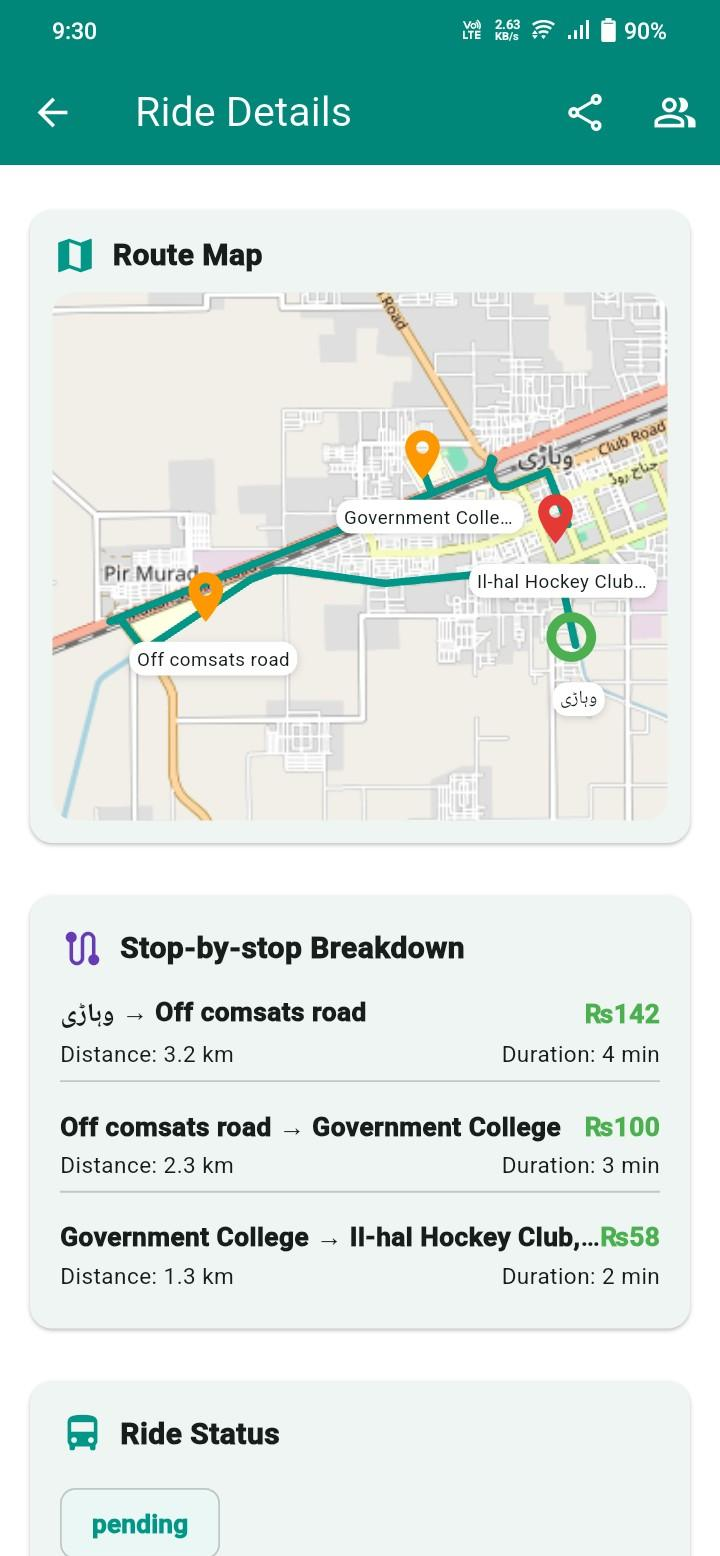
\includegraphics[width=\textwidth,height=0.52\textheight,keepaspectratio]{assets/app screenshot/driver_ride_details_pending_part1.jpeg}}
\end{minipage}\hfill
\begin{minipage}{0.45\textwidth}
\centering
\fbox{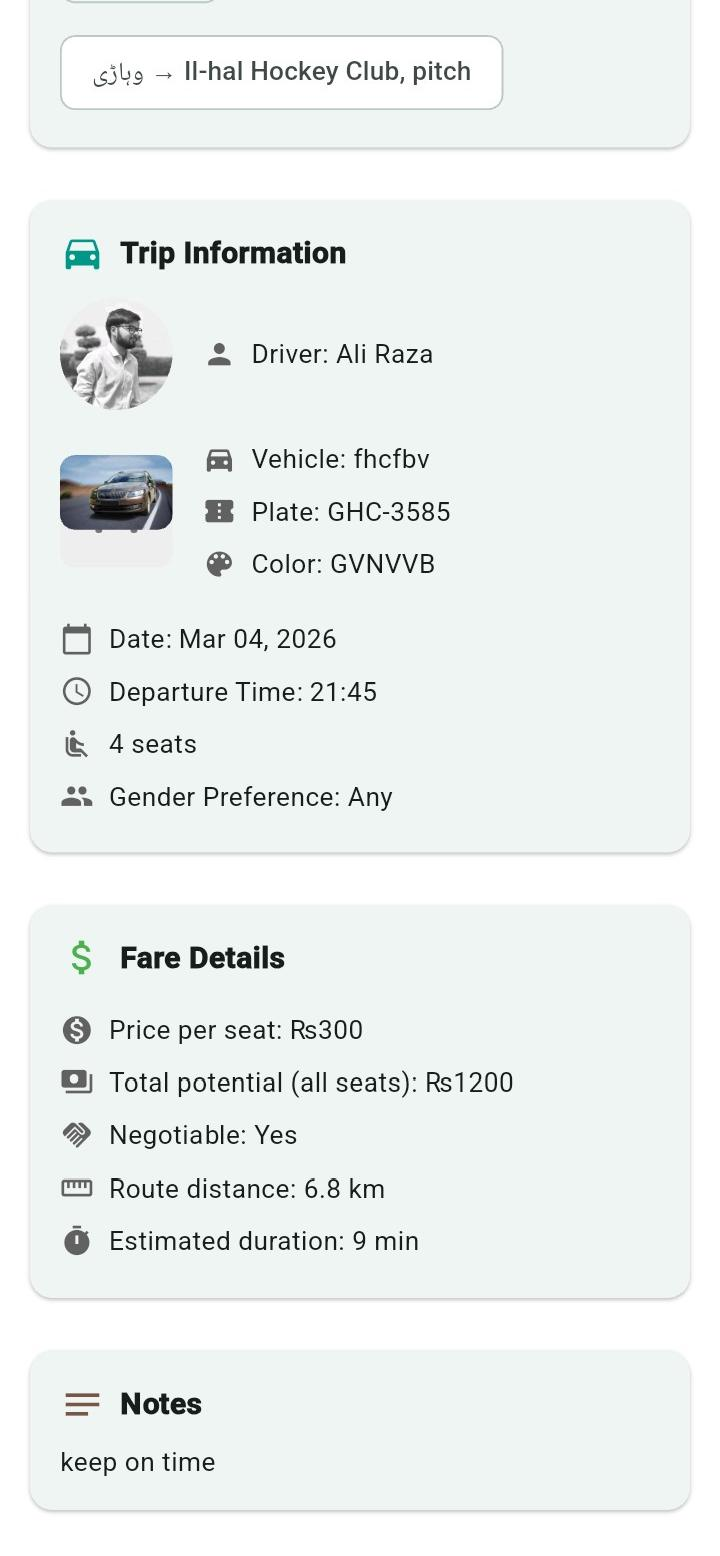
\includegraphics[width=\textwidth,height=0.52\textheight,keepaspectratio]{assets/app screenshot/driver_ride_details_pending_part2.jpeg}}
\end{minipage}
\caption{Driver Ride Details (Pending)}
\end{figure}

Functional Flow: Driver sees the work order and accepts/rejects or takes up negotiation. Passenger facing status updates instantly when driver actions are done.

\textbf{Backend Integration:} Driver actions are made to a booking decision Endpoint that updates booking status and sends notifications.

\textbf{Validation/Security:} only the trip owner can approve requests, backend checks prevent requests if there are not enough seats available.

\subsubsection{Screen 23: Negotiation Completed}

\textbf{Purpose:} Confirms that the negotiation is finalized and the booking request is accepted by both driver and passenger.

\textbf{Components:}
\begin{itemize}
    \item Acceptance confirmation and updated request status.
\end{itemize}

\begin{figure}[H]
\centering
\begin{minipage}{0.45\textwidth}
\centering
\fbox{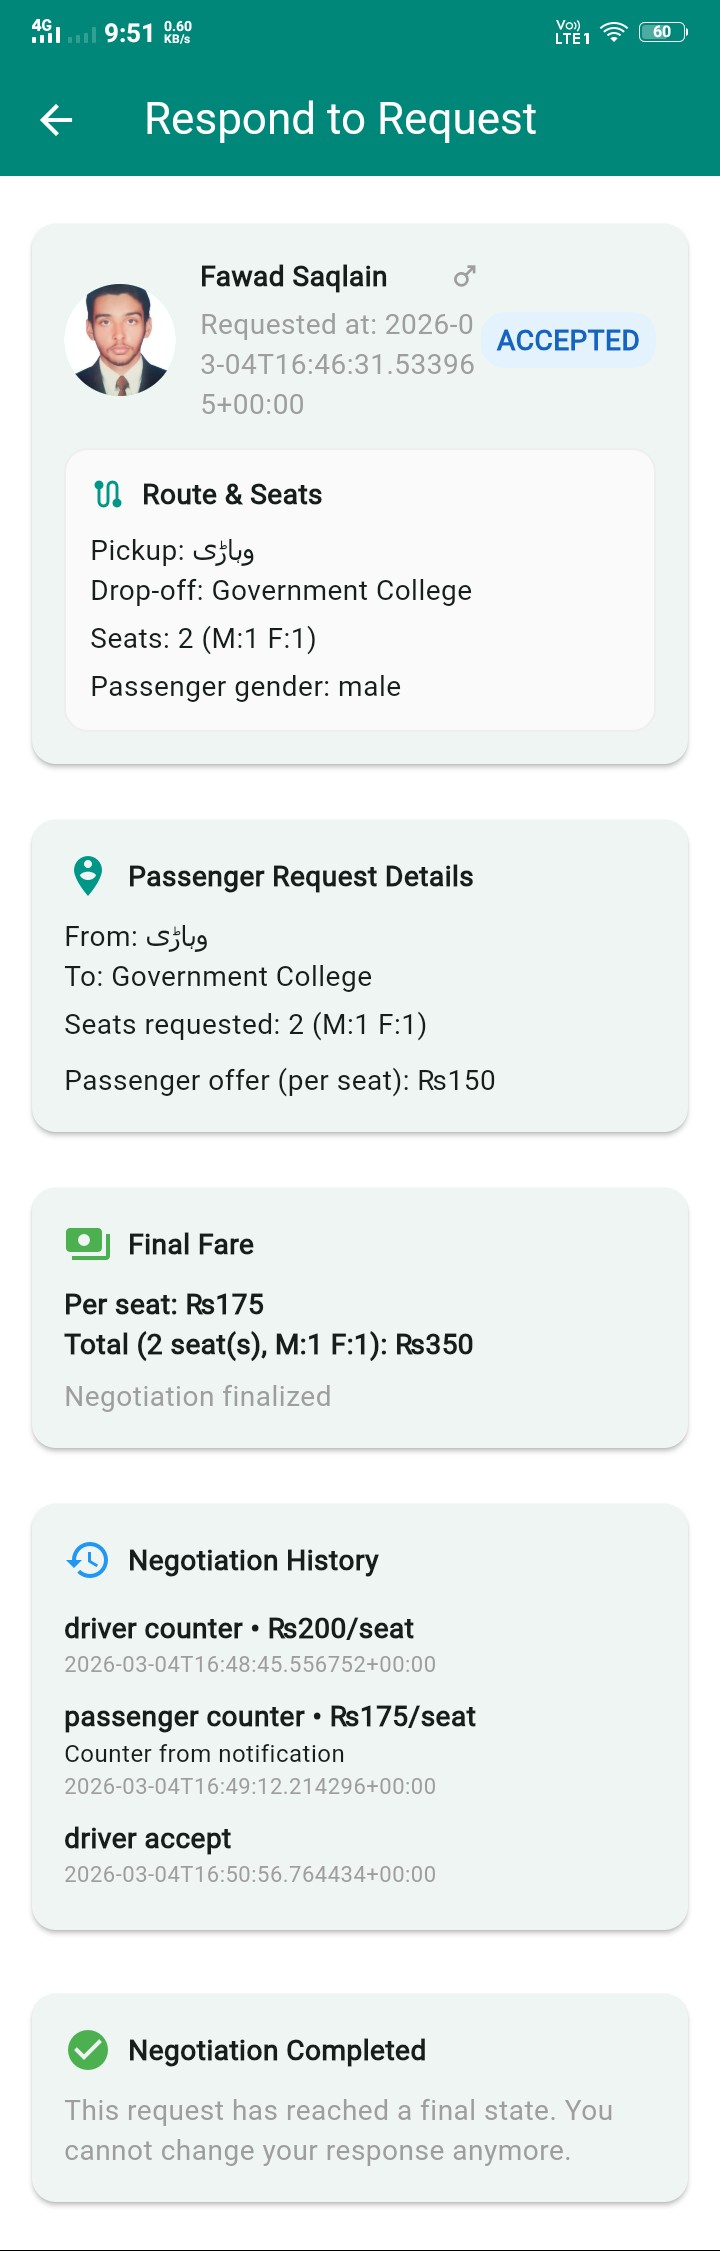
\includegraphics[width=\textwidth,height=0.65\textheight]{assets/app screenshot/driver_respond_request_accepted.jpeg}}
\end{minipage}\hfill
\begin{minipage}{0.45\textwidth}
\centering
\fbox{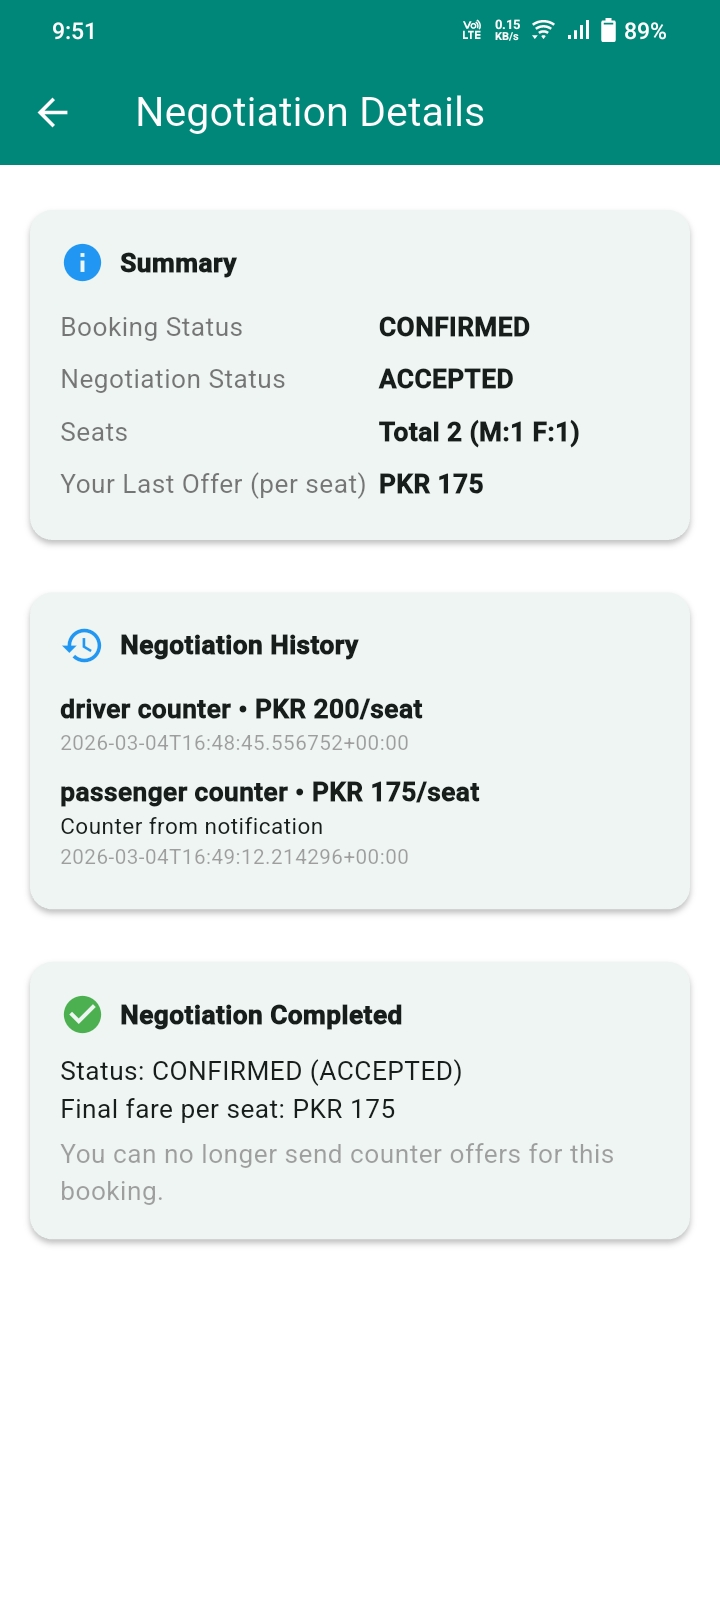
\includegraphics[width=\textwidth,height=0.65\textheight]{assets/app screenshot/passenger request accepted.jpg}}
\end{minipage}
\caption{Negotiation Completed}
\end{figure}

Accepted/Confirmed Booking: If both parties agree to the final terms, the booking moves to the accepted/confirmed state. The next steps open up – including chat, ride tracking, and, later, payments confirmation.

\textbf{Backend Integration:} When a user accepts it, it is stored in the booking and downstream (notifications, lock seats, etc. and tracking readiness of the session).

\textbf{Validation/Security:} Backend validates that acceptance may take place from valid negotiation states and from authorized users.

\subsubsection{Screen 24: My Rides}

\textbf{Function:} Providing users with a dashboard where they can view their future and current trips commitments.

\textbf{Components:}
\begin{itemize}
    \item Active ride cards with quick actions such as Chat and Tracking.
\end{itemize}

\begin{figure}[H]
\centering
\begin{minipage}{0.45\textwidth}
\centering
\fbox{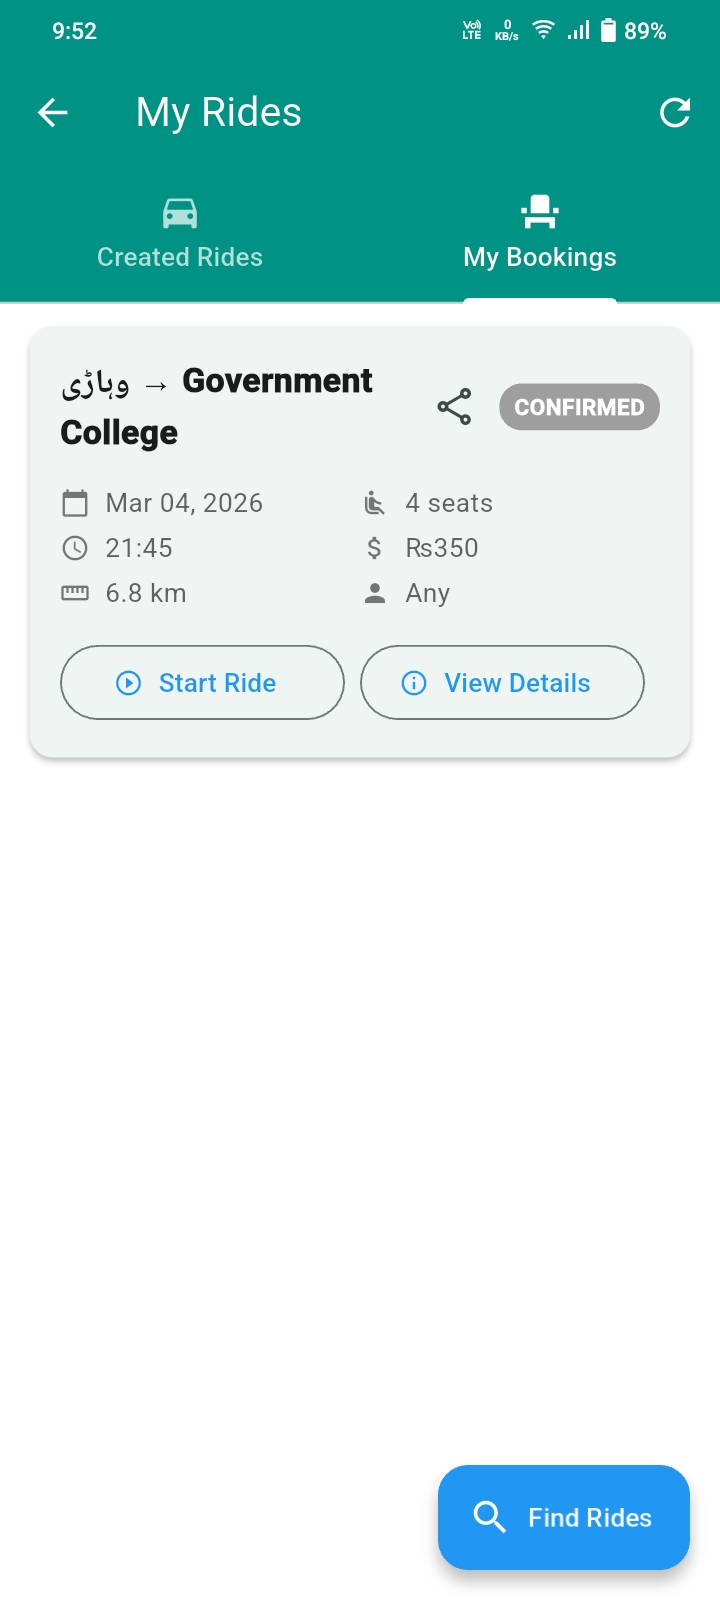
\includegraphics[width=\textwidth,height=0.65\textheight,keepaspectratio]{assets/app screenshot/my_bookings_confirmed.jpeg}}
\end{minipage}\hfill
\begin{minipage}{0.45\textwidth}
\centering
\fbox{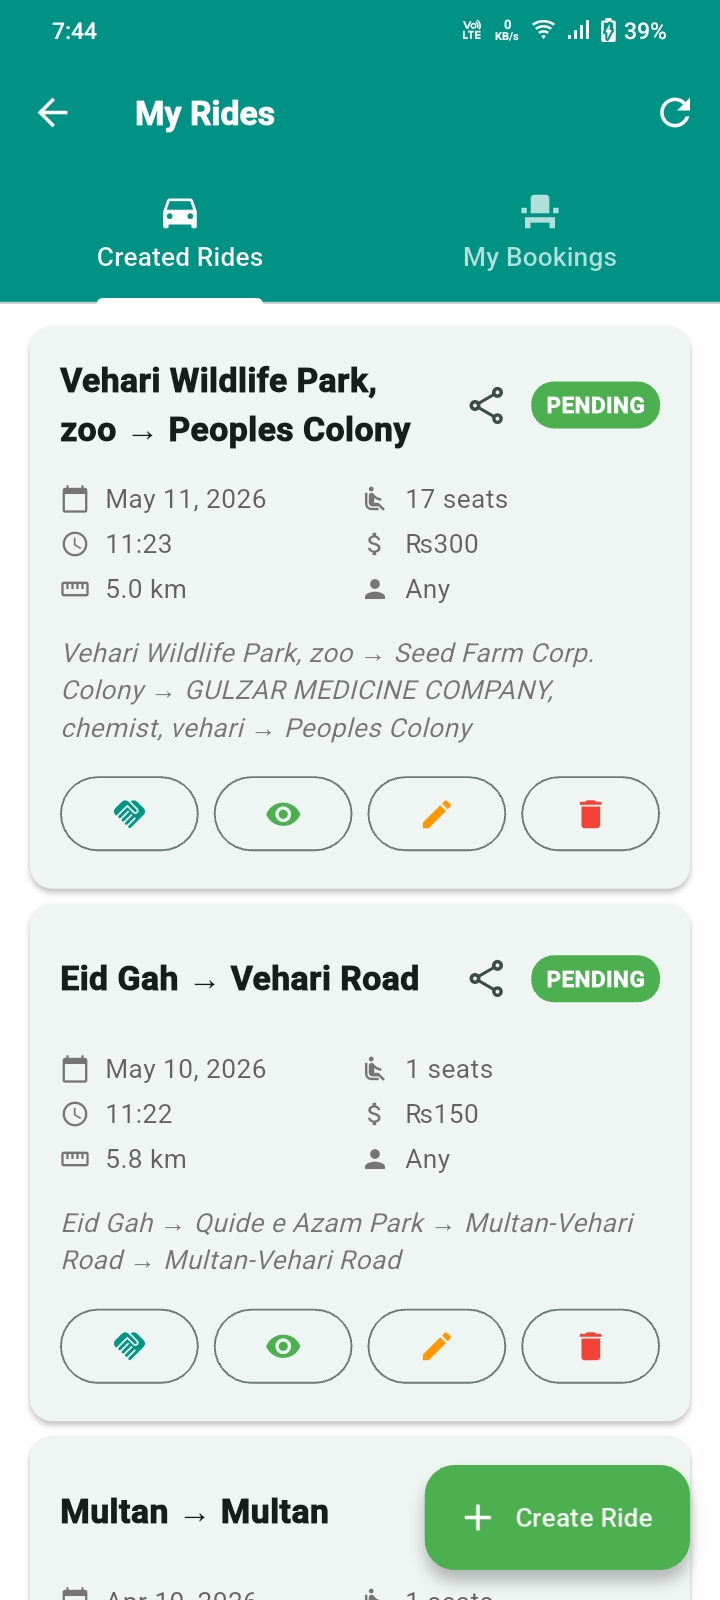
\includegraphics[width=\textwidth,height=0.65\textheight,keepaspectratio]{assets/app screenshot/my rides created rides.jpg}}
\end{minipage}
\caption{My Rides}
\end{figure}

The functional flow will let users see all their currently active and upcoming rides from one list and launch actions like chat, tracking etc. This screen is the primary one for post-booking operations.

\textbf{Backend Integration:} Fetches ride list from booking and trip history endpoints, and filters by status.

\textbf{Validation/Security:} Results are filtered for the authenticated user and sensitive data is obscured by roles.

\subsubsection{Screen 25: Live Tracking and Pickup Verification}

This screen provides live tracking and pick-up verification.This screen offers live tracking and pick-up verification.

\textbf{Goal:} Real time monitoring of an active ride for driver and passenger, secure pickup verification.

\textbf{Components:}
\begin{itemize}
    \item GPS Markers for vehicle and pickup location.
    \item Periodic ETA updates.
    \item QR Code verification for pickups.
\end{itemize}

\begin{figure}[H]
\centering
\begin{minipage}{0.30\textwidth}
\centering
\fbox{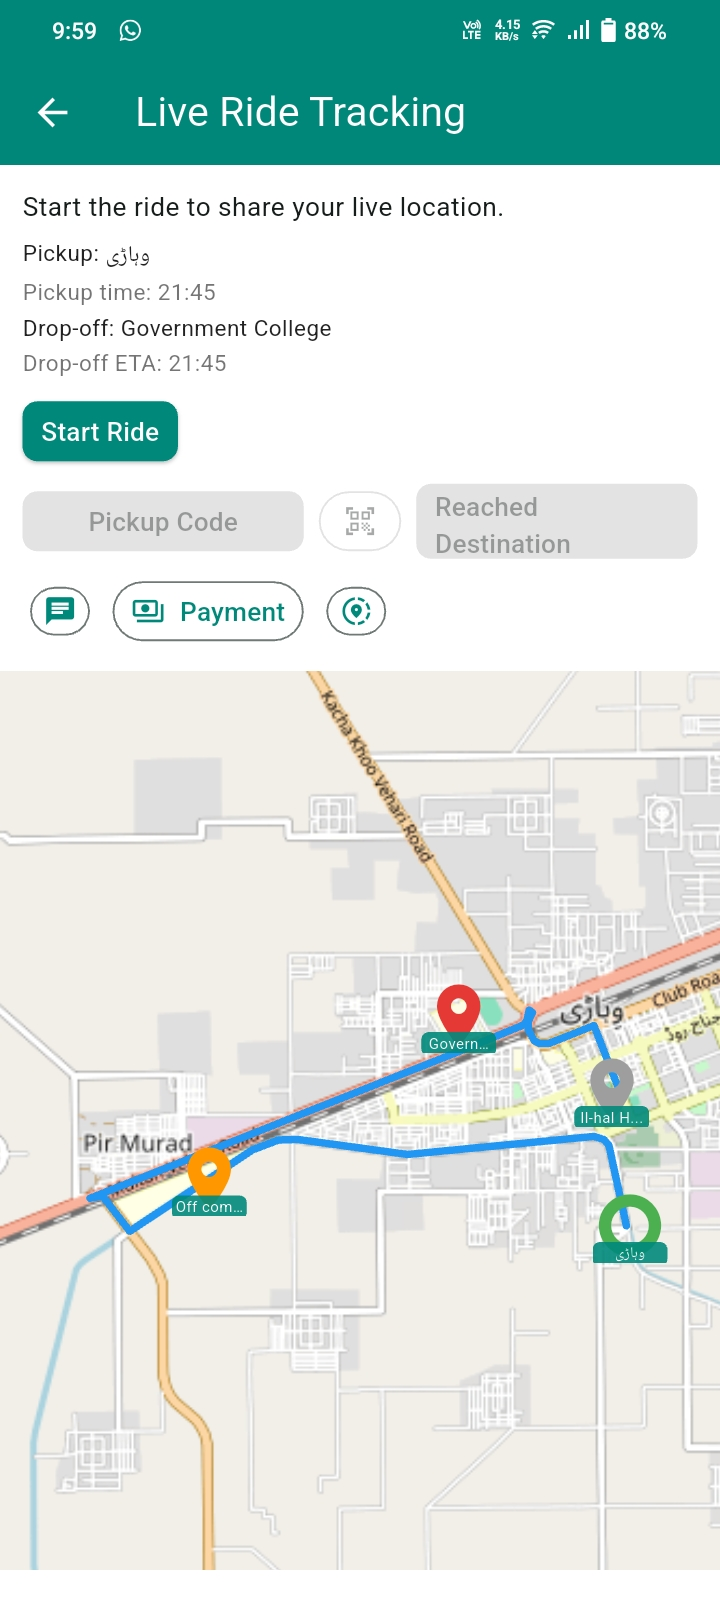
\includegraphics[width=\textwidth,keepaspectratio]{assets/app screenshot/passenger_live_tracking_start.jpeg}}
\end{minipage}\hfill
\begin{minipage}{0.30\textwidth}
\centering
\fbox{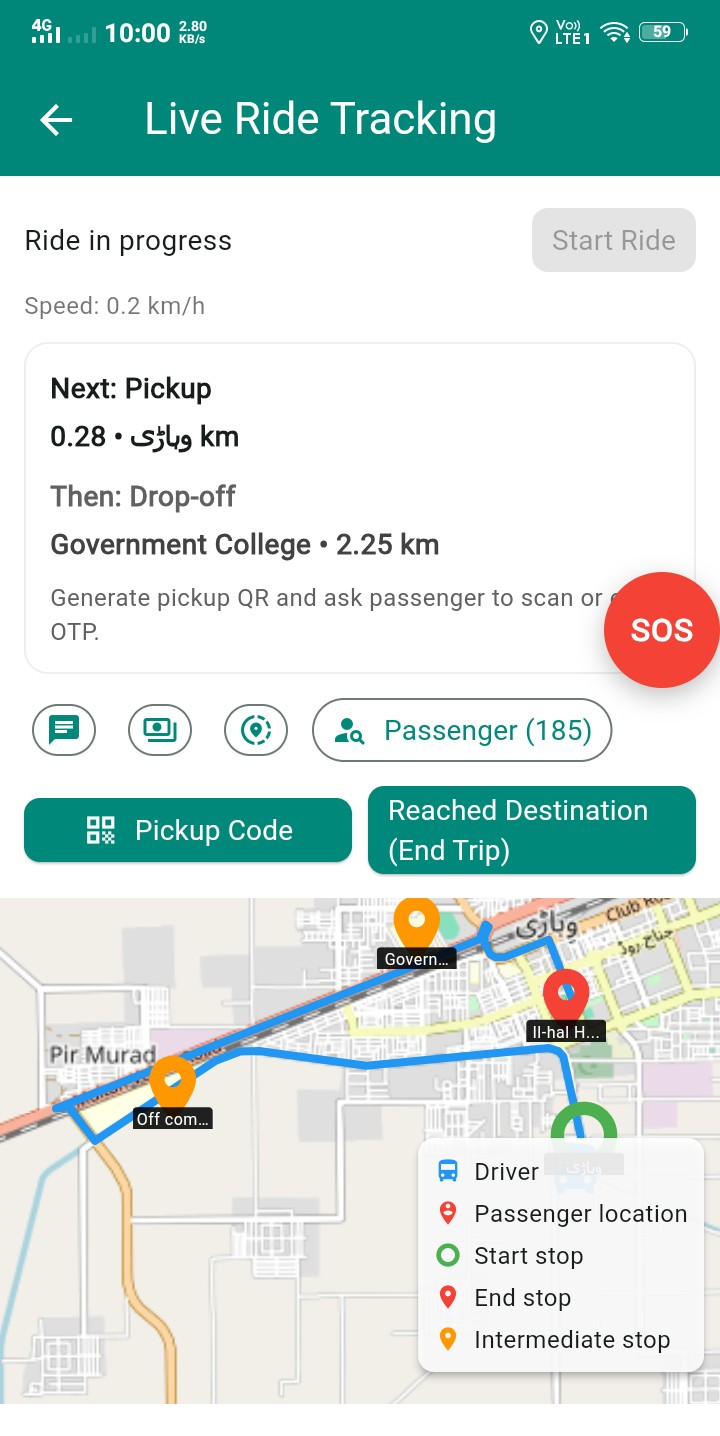
\includegraphics[width=\textwidth,keepaspectratio]{assets/app screenshot/driver_live_ride_tracking.jpeg}}
\end{minipage}\hfill
\begin{minipage}{0.30\textwidth}
\centering
\fbox{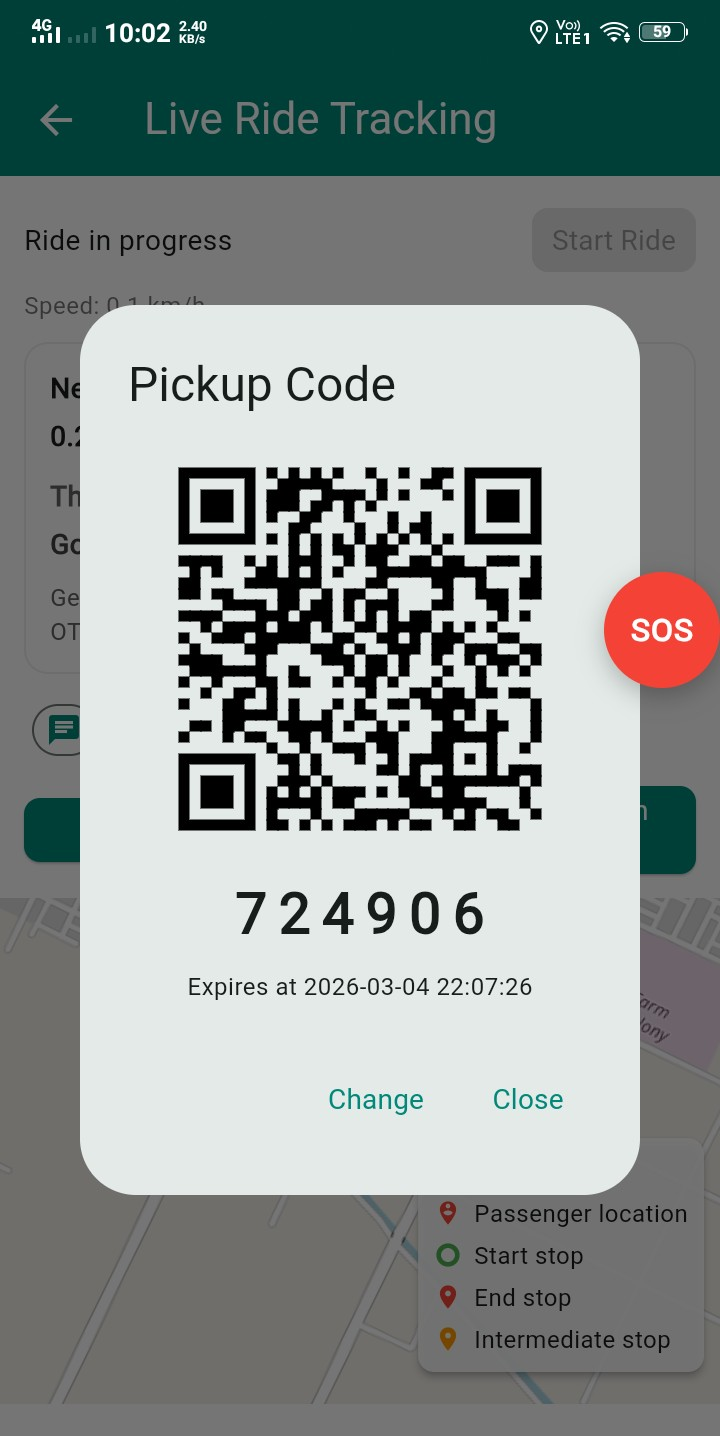
\includegraphics[width=\textwidth,keepaspectratio]{assets/app screenshot/driver_pickup_qr_code.jpeg}}
\end{minipage}
\caption{Passenger Live Tracking, Driver Live Tracking, and Driver Pickup QR Code}
\end{figure}

Figure 5.13 is a passenger live tracking, driver live tracking, and driver pick up QR code.

The QR code is checked for boarding at pickup before heading on to the process.

\textbf{Tracking:} Periodic location updates through API calls and bookings and trip identifier to get the live state of the session.

\textbf{Validation/Security:} Only users on the active booking can access the tracking, pickup verification prevents unauthorized boarding.

\subsubsection{Screen 29: Payment and Rating Screen}

The Payment and Rating Screen opens.The Payment and Rating screen appears.

\textbf{Use:} Allows riders to pay, rate after a ride and for the driver to acknowledge receipt of payment.

\textbf{Components:}
\begin{itemize}
    \item Choice and confirmation of payment method and final amount.
    \item Submitting a rating following payment.
    \item Receipt confirmation on driver.
\end{itemize}

\begin{figure}[H]
\centering
\begin{minipage}{0.30\textwidth}
\centering
\fbox{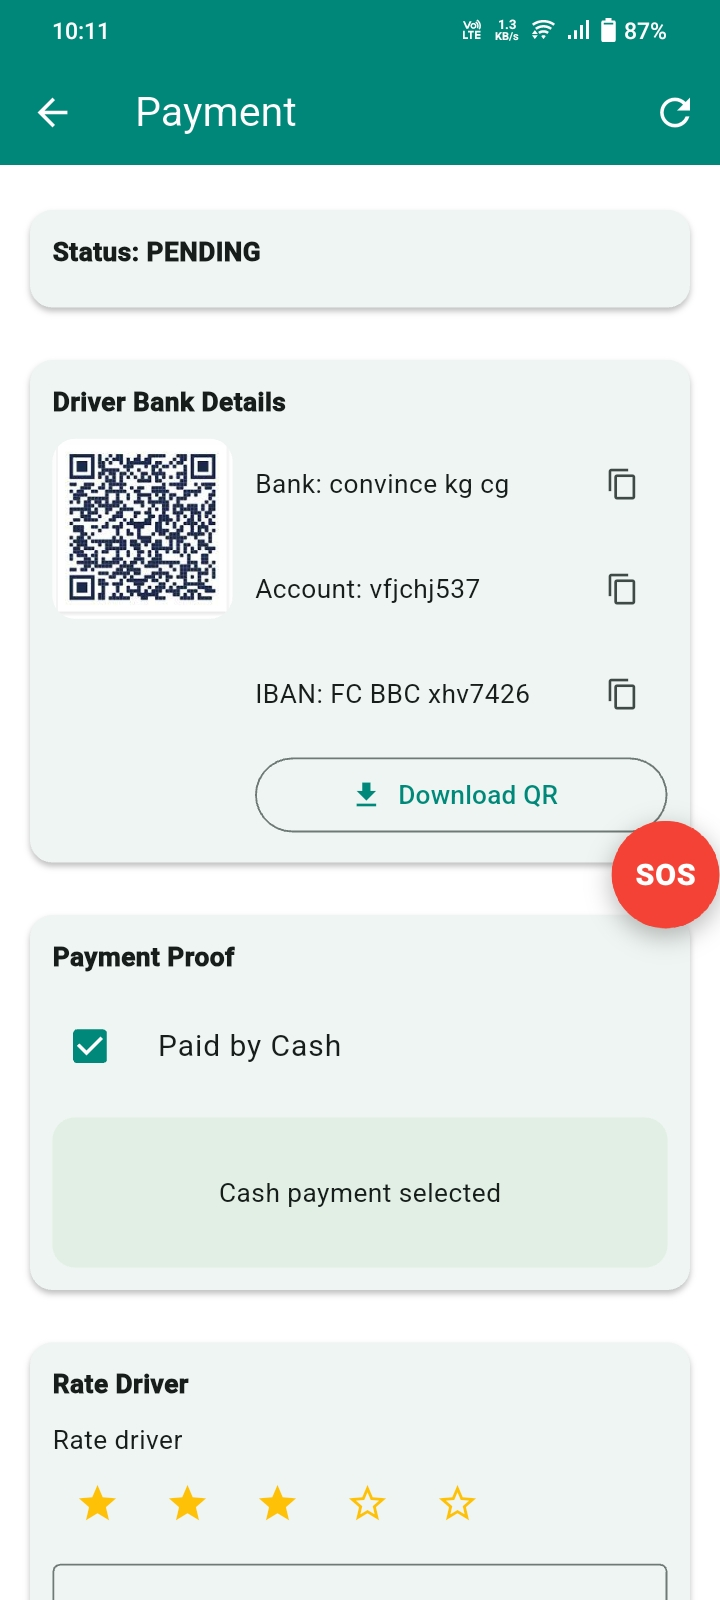
\includegraphics[width=\textwidth,keepaspectratio]{assets/app screenshot/payment_screen_cash.jpeg}}
\end{minipage}\hfill
\begin{minipage}{0.30\textwidth}
\centering
\fbox{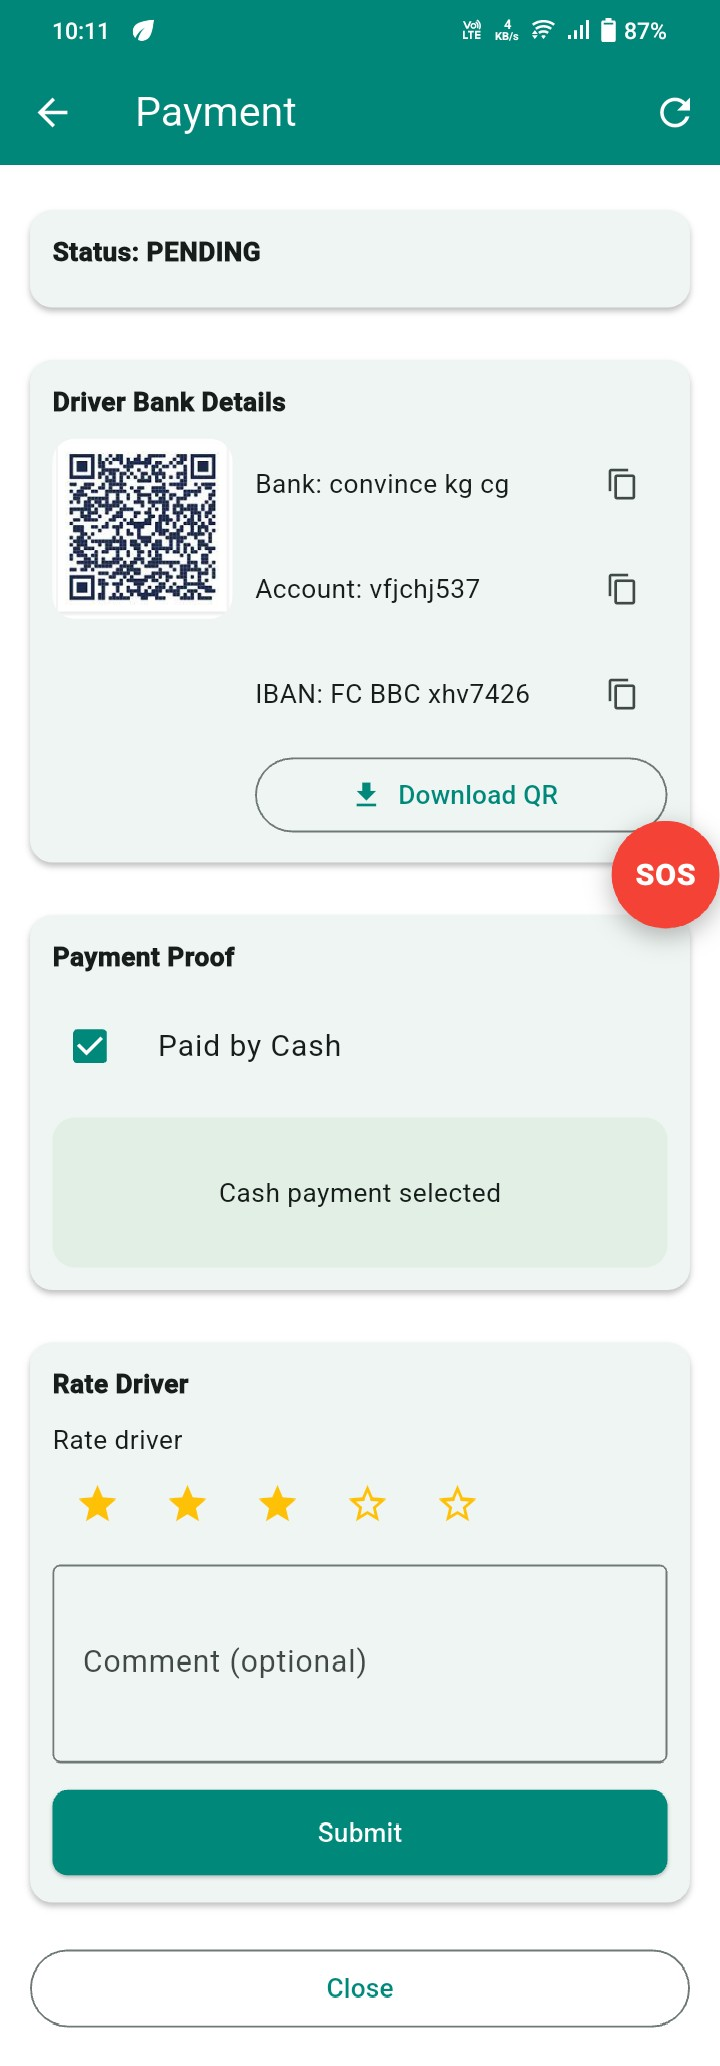
\includegraphics[width=\textwidth,height=0.55\textheight]{assets/app screenshot/passenger payment and rating screen.jpeg}}
\end{minipage}\hfill
\begin{minipage}{0.30\textwidth}
\centering
\fbox{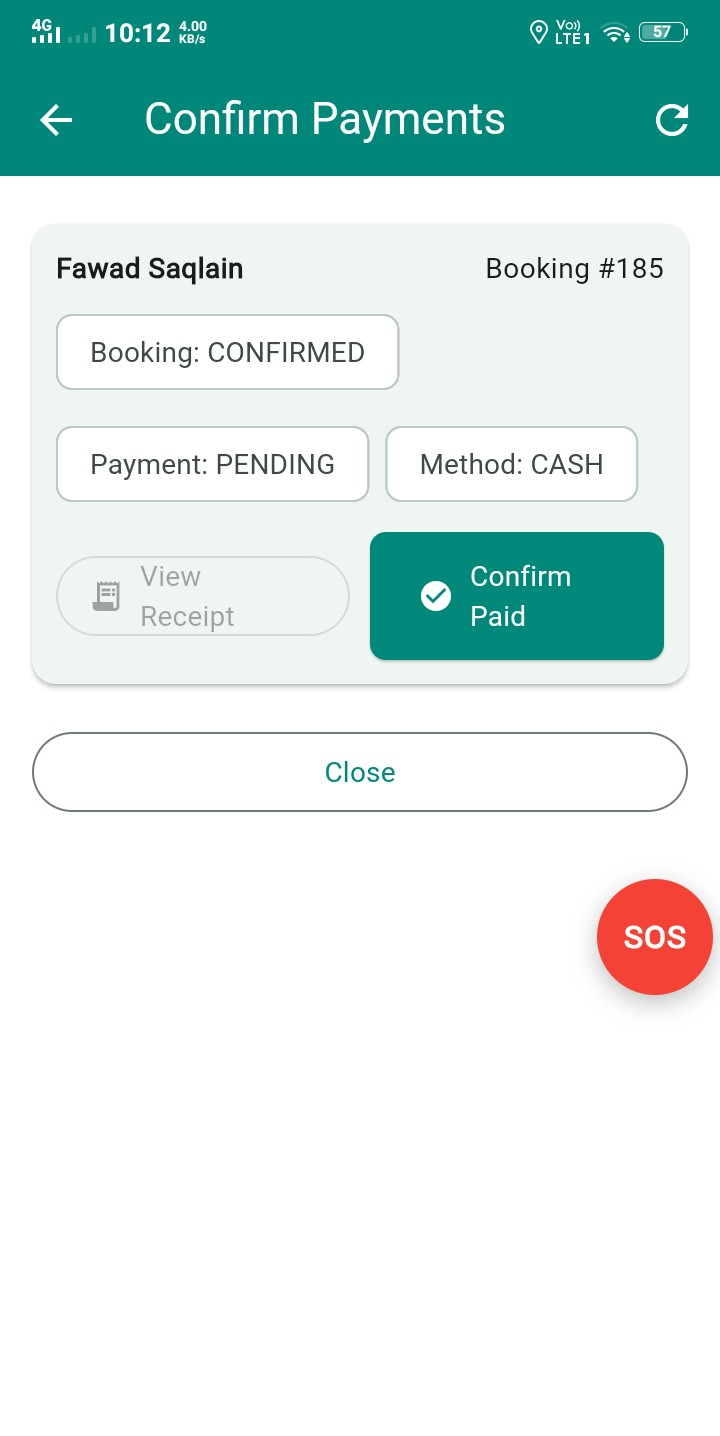
\includegraphics[width=\textwidth,keepaspectratio]{assets/app screenshot/driver_confirm_payments.jpeg}}
\end{minipage}
\caption{Passenger Payment, Rating, and Driver Payment Confirmation}
\end{figure}

Once the driver has confirmed receipt, the booking is complete.

\textbf{Backend Integration:} Payment submit / payment confirm endpoints that are coupled to the booking/payment records.

\textbf{Validation/Security:} Confirmation permissions are role based and there is no double confirmation.

\subsubsection{Screen 31: Messaging and User Chat}

Messaging and User Chat:Screen 31: Messaging and User Chat:

The purpose is to provide unified communication system for drivers to communicate with passengers.

\textbf{Components:}
\begin{itemize}
    \item Bubble chat where bubbles are marked with a time.
\end{itemize}

\begin{figure}[H]
\centering
\begin{minipage}{0.30\textwidth}
\centering
\fbox{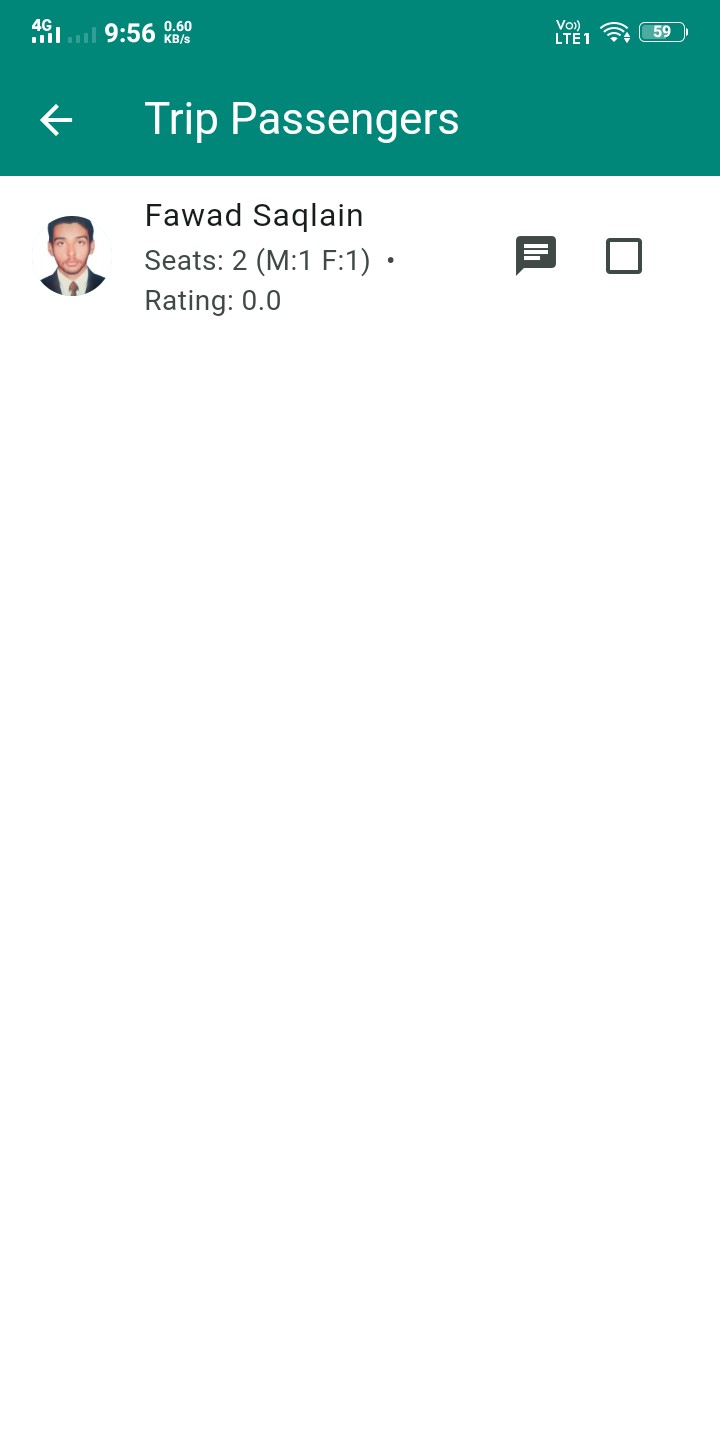
\includegraphics[width=\textwidth,keepaspectratio]{assets/app screenshot/driver_trip_passengers_list.jpeg}}
\end{minipage}\hfill
\begin{minipage}{0.30\textwidth}
\centering
\fbox{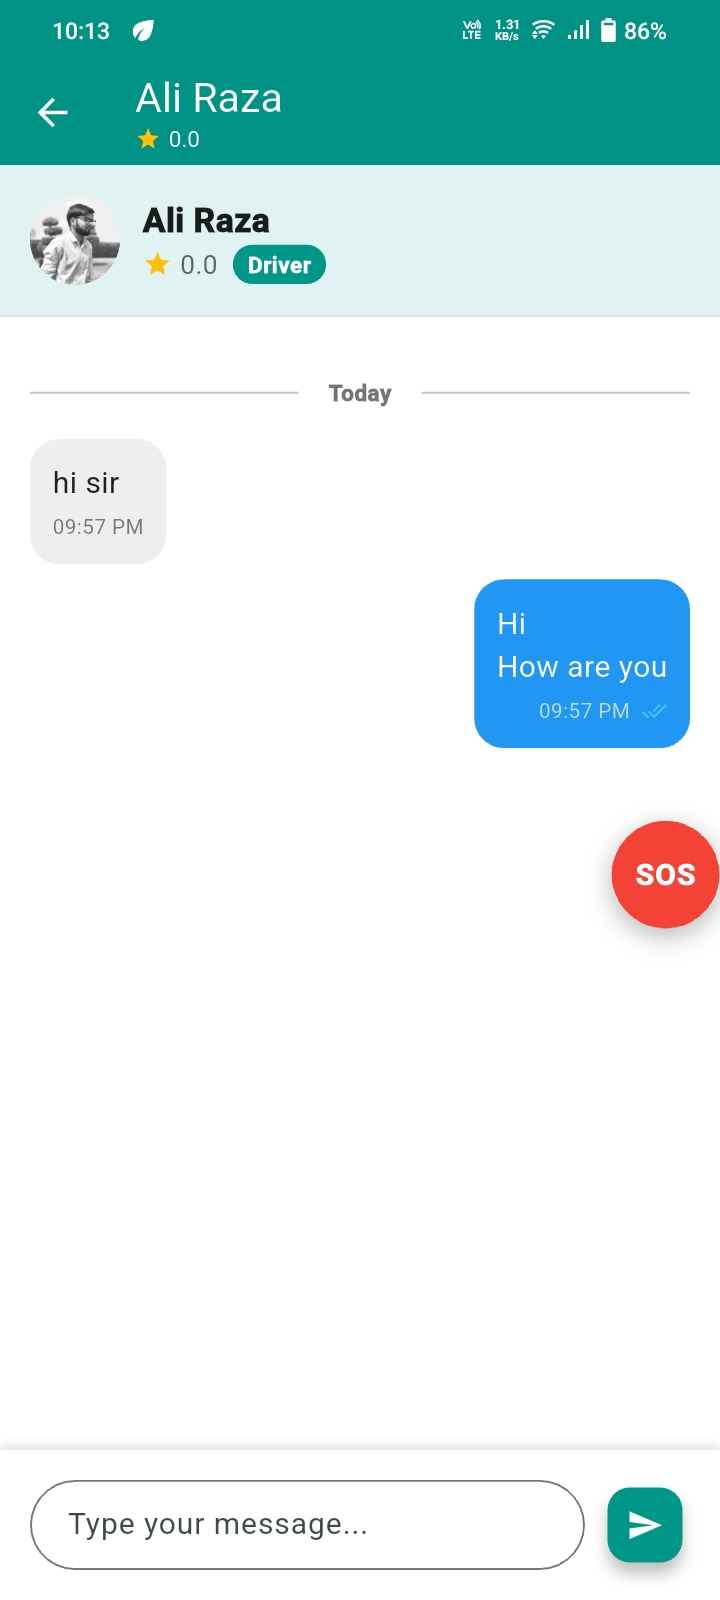
\includegraphics[width=\textwidth,keepaspectratio]{assets/app screenshot/passenger_driver_one_to_one_chating_screen.jpeg}}
\end{minipage}\hfill
\begin{minipage}{0.30\textwidth}
\centering
\fbox{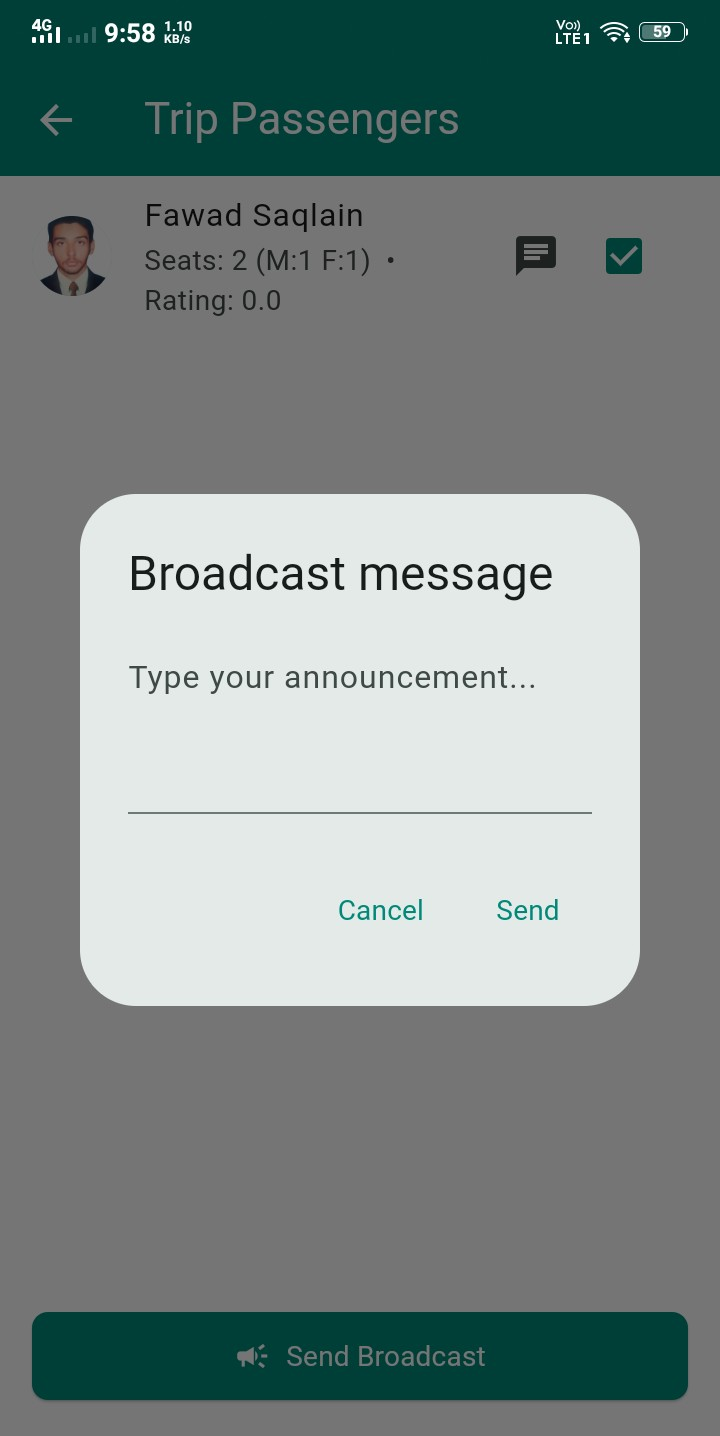
\includegraphics[width=\textwidth,keepaspectratio]{assets/app screenshot/driver_broadcast_message.jpeg}}
\end{minipage}
\caption{Messaging and User Chat}
\end{figure}

Booking and ride execution involves functional flow: Drivers and passengers are exchanging messages for coordination and updates. Broadcast messages can be used to send information to ALL passengers on a trip.

\textbf{Backend Integration:} Messaging stores messages for future retrieval and does so through chat service endpoints.

\textbf{Validation/Security:} Messages can only be seen by participants in the same trip/booking, and message filters are based on the roles of the participants.

\subsubsection{Screen 32: Support Chat - Bot \& Admin}

On screen \#32, you can click on the Support Chat-Bot \& Admin button.Click Support Chat-Bot \& Admin on screen \#32.

\textbf{Goal:} A dedicated channel for platform support and manual resolution.

\textbf{Components:}
\begin{itemize}
    \item Bot response options and live Admin escalation.
\end{itemize}

\begin{figure}[H]
\centering
\begin{minipage}{0.45\textwidth}
\centering
\fbox{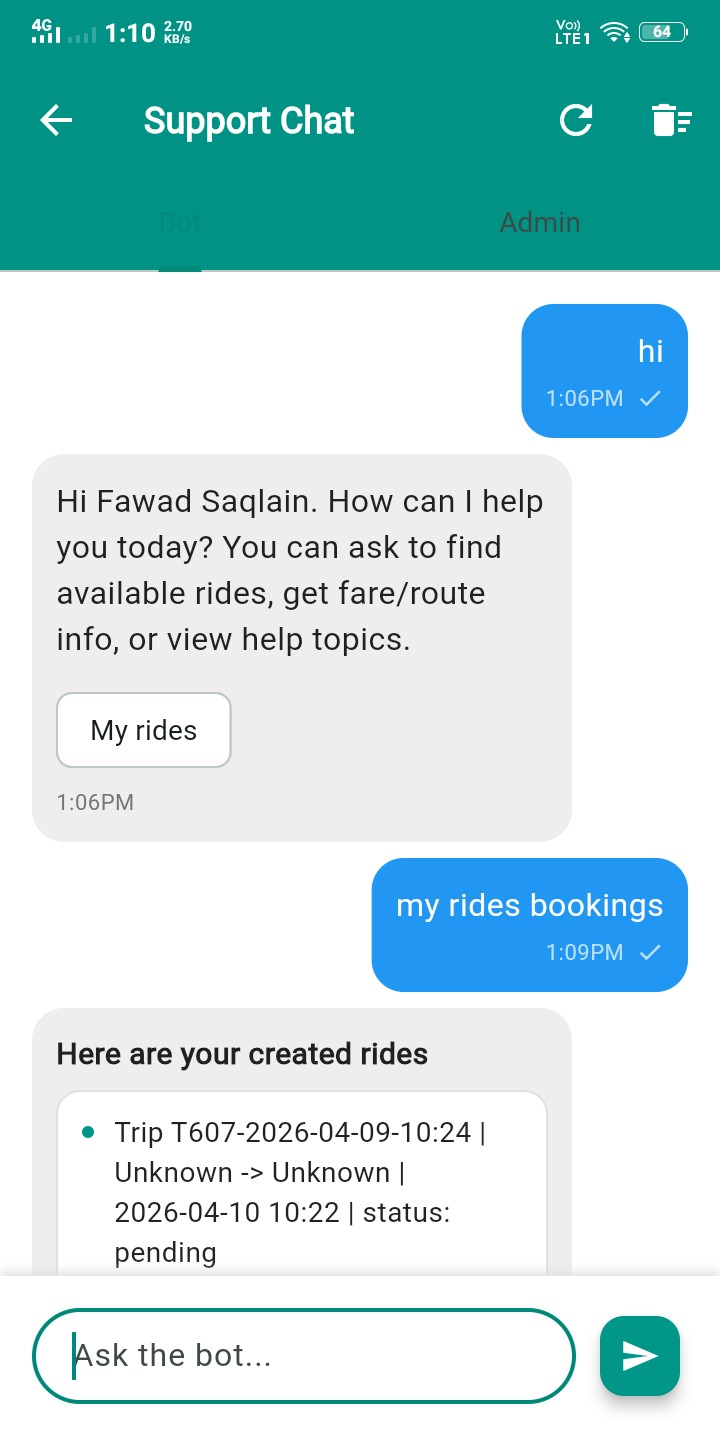
\includegraphics[width=\textwidth,keepaspectratio]{assets/app screenshot/support_chat_bot.jpeg}}
\end{minipage}\hfill
\begin{minipage}{0.45\textwidth}
\centering
\fbox{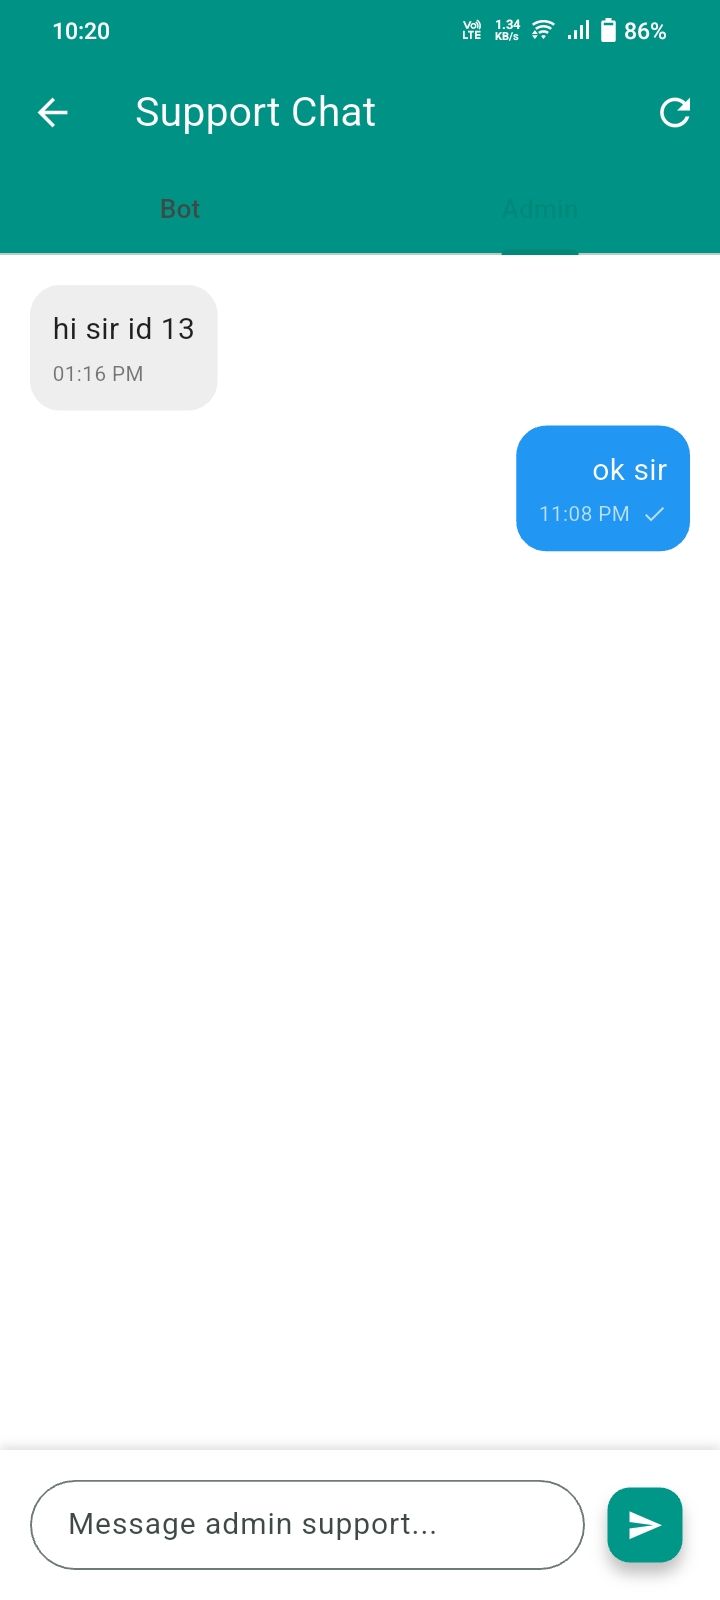
\includegraphics[width=\textwidth,keepaspectratio]{assets/app screenshot/support_chat_admin_reply.jpeg}}
\end{minipage}
\caption{Support Chat - Bot \& Admin}
\end{figure}

The user first contacts the support bot to resolve common issues and guided troubleshooting. If it is a manual handling problem, it is discussed in an Admin support channel to resolve the issue.

\textbf{Backend Integration:} The screen loads and posts messages with support chat endpoints, and fetches new replies periodically.

\textbf{Validation/Security:} access restricted to authenticated user (or guest support session) and message threads (chats) isolated per user.

\subsubsection{Screen 33: Notifications List}

\textbf{Description:} All System Alerts for all Users are fed in chronological order.

\textbf{Components:}
\begin{itemize}
    \item Deep link notification cards.
\end{itemize}

\begin{figure}[H]
\centering
\begin{minipage}{0.45\textwidth}
\centering
\fbox{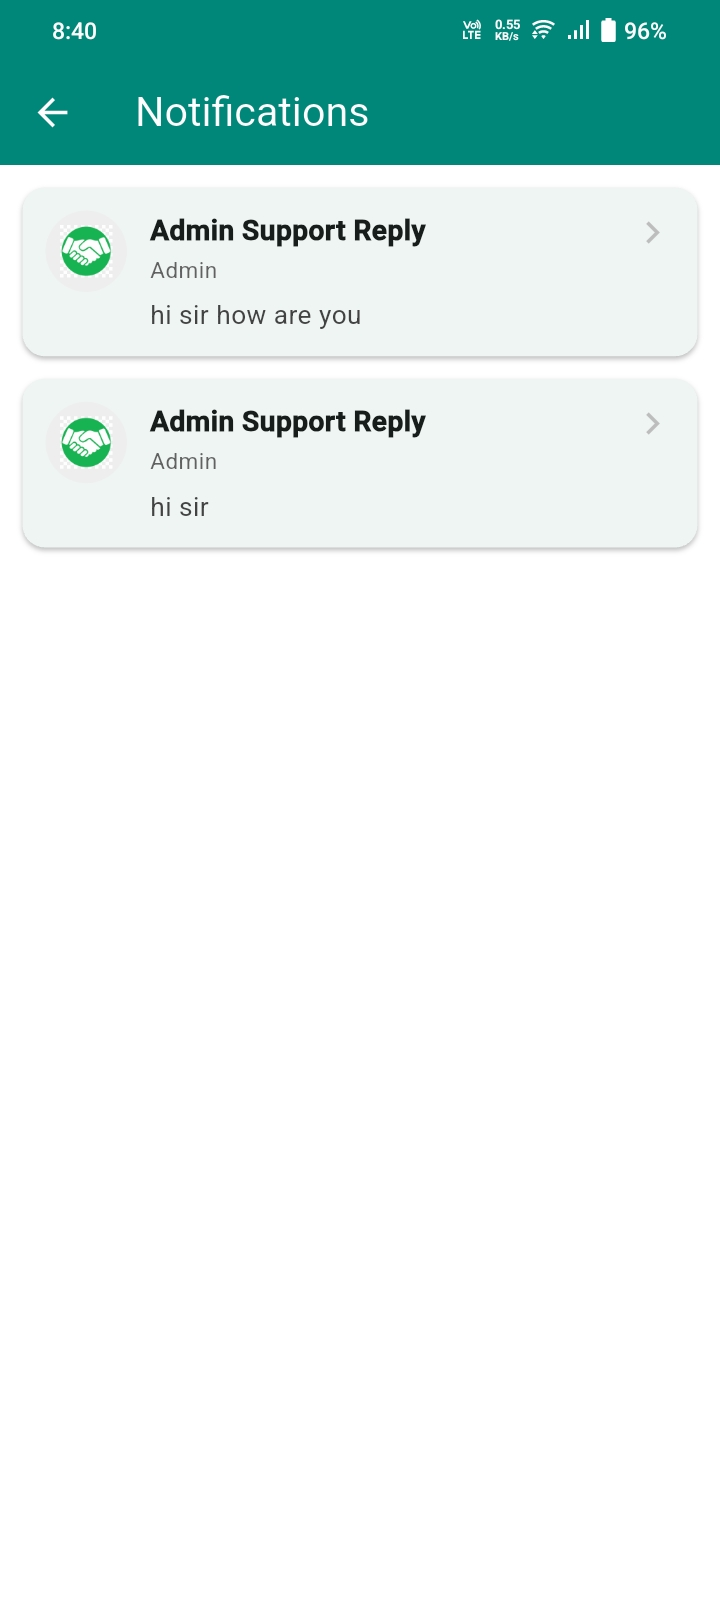
\includegraphics[width=\textwidth,height=0.66\textheight,keepaspectratio]{assets/app screenshot/notifications_list.jpeg}}
\end{minipage}\hfill
\begin{minipage}{0.45\textwidth}
\centering
\fbox{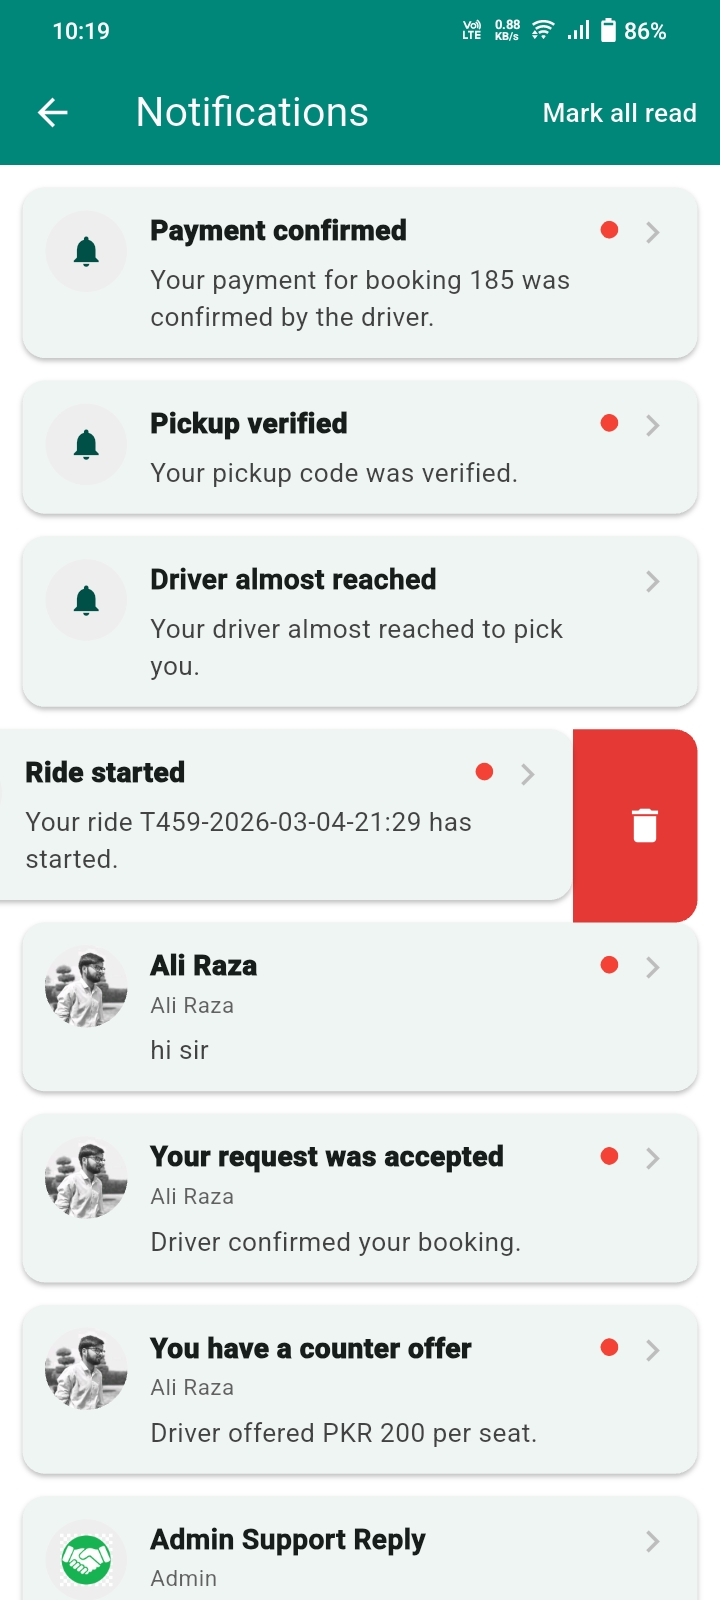
\includegraphics[width=\textwidth,height=0.66\textheight,keepaspectratio]{assets/app screenshot/notification_deletion.jpeg}}
\end{minipage}
\caption{Notifications List}
\end{figure}

Functional Flow: User opens the notifications inbox to check updates on booking, SOS alerts, and system announcements. Deep-links direct users to the relevant screen and notifications can be viewed and dismissed.

\textbf{Backend Integration:} Notifications are retrieved from the backend notifications API and refreshed periodically, or when triggered by FCM.

\textbf{Validation/Security:} Only the current user's notifications returned and sensitive payload data filtered by role and ownership.

\subsubsection{Screen 34-35: Emergency SOS}

The purpose is to provide intervener to user with tool to intervene in the immediate moment of distress.

\textbf{Components:}
\begin{itemize}
    \item Visual confirmation of countdown and alarm.
\end{itemize}

\begin{figure}[H]
\centering
\begin{minipage}{0.30\textwidth}
\centering
\fbox{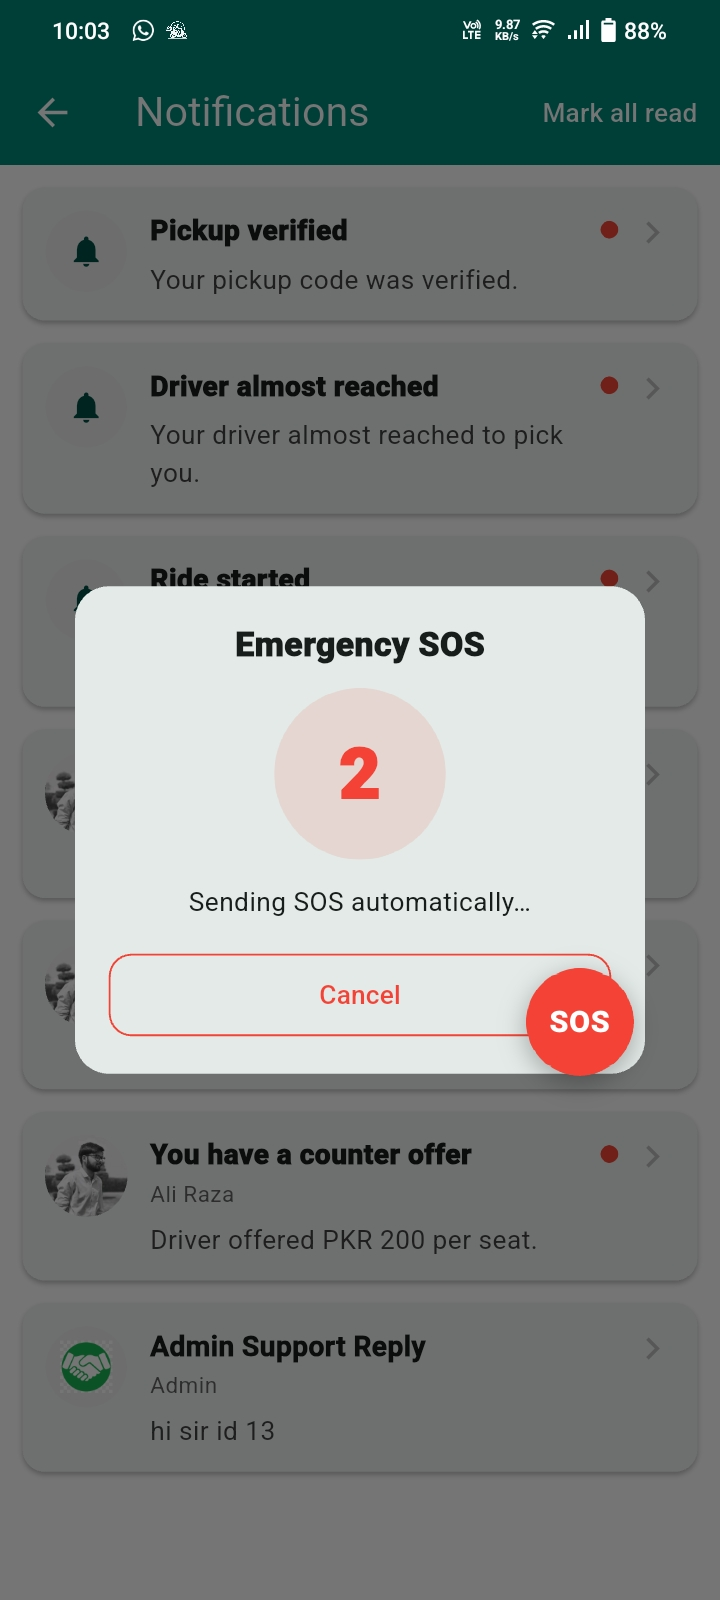
\includegraphics[width=\textwidth,keepaspectratio]{assets/app screenshot/emergency_sos_countdown.jpeg}}
\end{minipage}\hfill
\begin{minipage}{0.30\textwidth}
\centering
\fbox{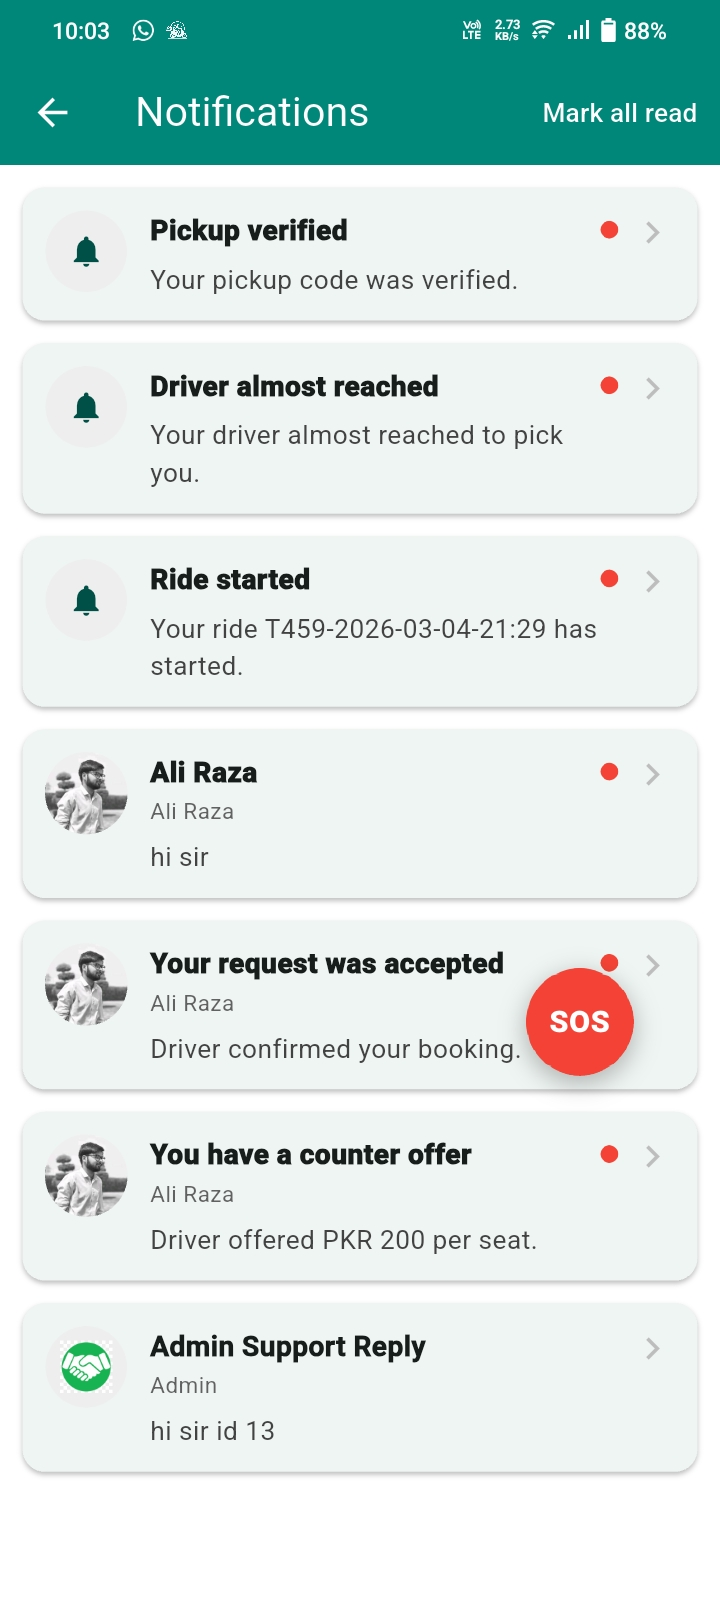
\includegraphics[width=\textwidth,keepaspectratio]{assets/app screenshot/notifications_list_sos.jpeg}}
\end{minipage}\hfill
\begin{minipage}{0.30\textwidth}
\centering
\fbox{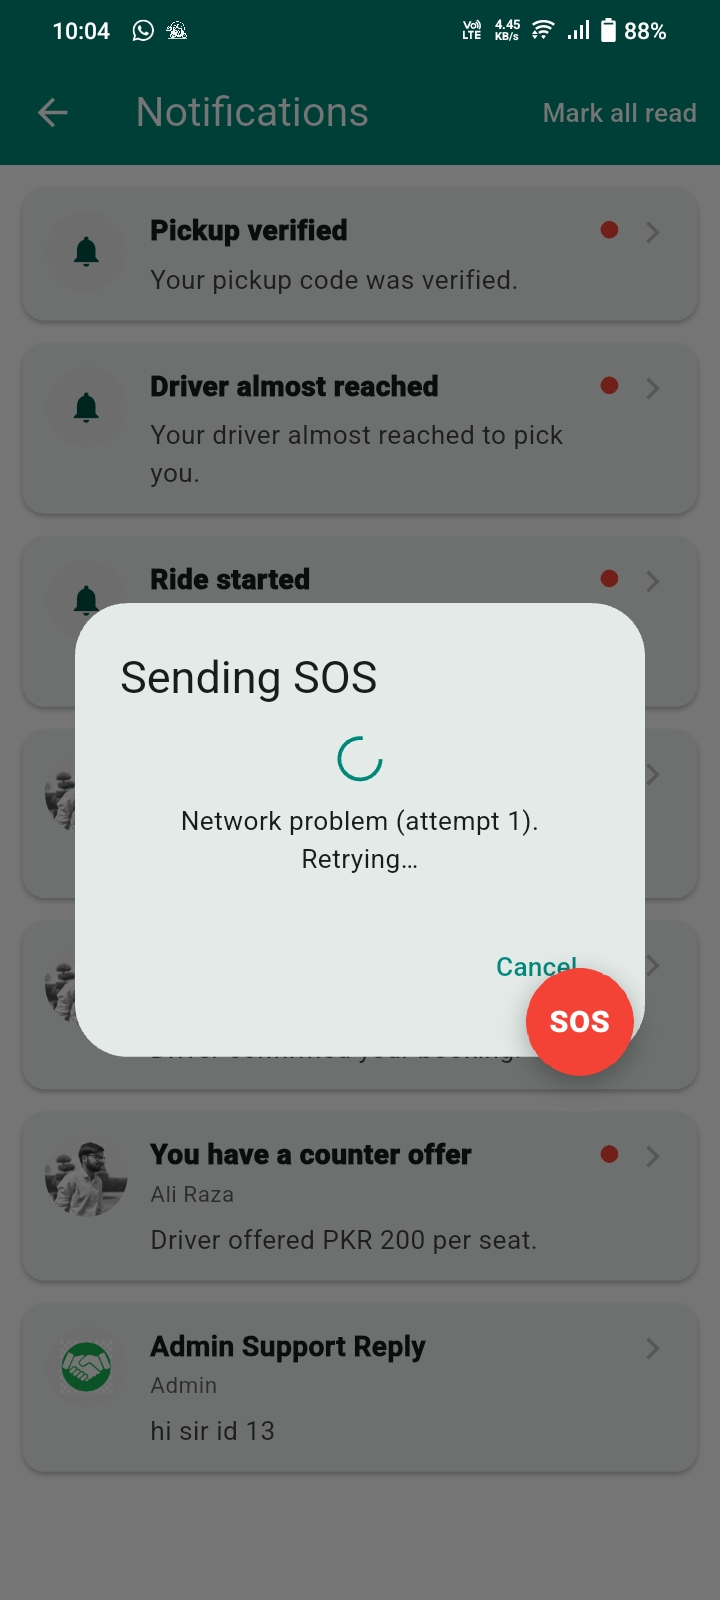
\includegraphics[width=\textwidth,keepaspectratio]{assets/app screenshot/emergency_sos_network_error.jpeg}}
\end{minipage}
\caption{Emergency SOS (Countdown, SOS Notifications, and Offline/Error State)}
\end{figure}

Functional Flow: User activates SOS, goes through the countdown confirmation, and the incident is documented and reported via SOS notifications. If there is an offline/connection error, the UI gives the user offline/connection advice until the request can be made.

\textbf{Backend Integration:} SOS events are sent to the back-end incident endpoints, and trigger notification entries to users and Admin monitoring.

\textbf{Validation/Security:} Requests for SOS are associated with the current session user, and subjected to rate limits, thereby preventing abuse; visibility of incidents are role-controlled.

\subsubsection{Screen 36: Profile Overview}

\textbf{Purpose:} Manage personal stats and application settings.

\textbf{Components:}
\begin{itemize}
    \item User profile card and navigation menu.
\end{itemize}

\begin{figure}[H]
\centering
\begin{minipage}{0.45\textwidth}
\centering
\fbox{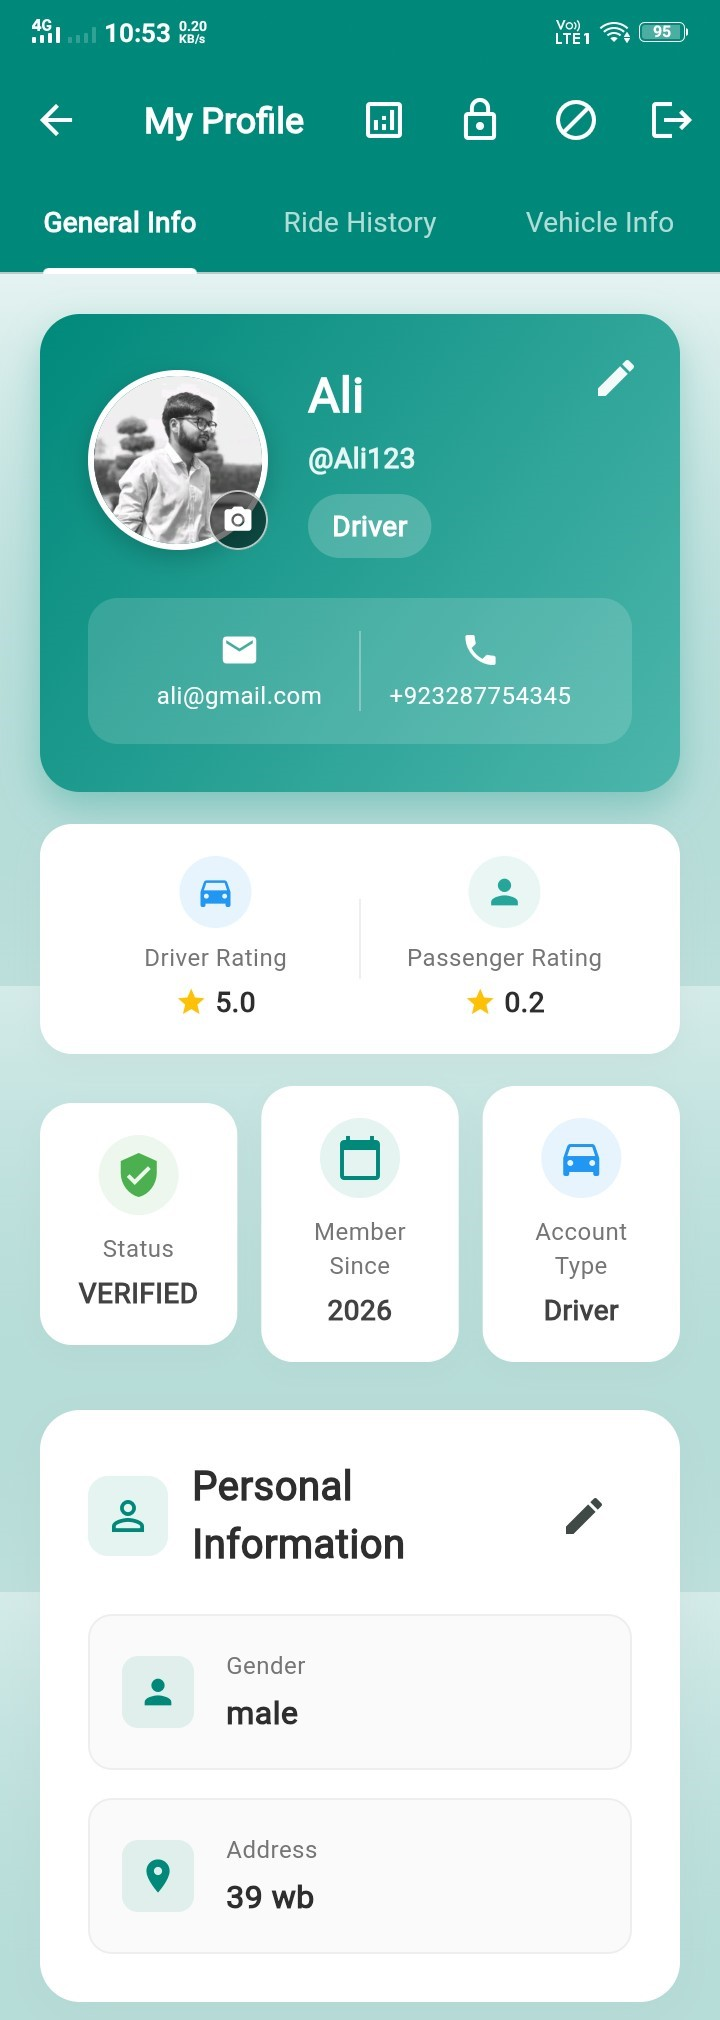
\includegraphics[width=\textwidth,height=0.8\textheight,keepaspectratio]{assets/app screenshot/profile_general_info_part1.jpeg}}
\end{minipage}\hfill
\begin{minipage}{0.45\textwidth}
\centering
\fbox{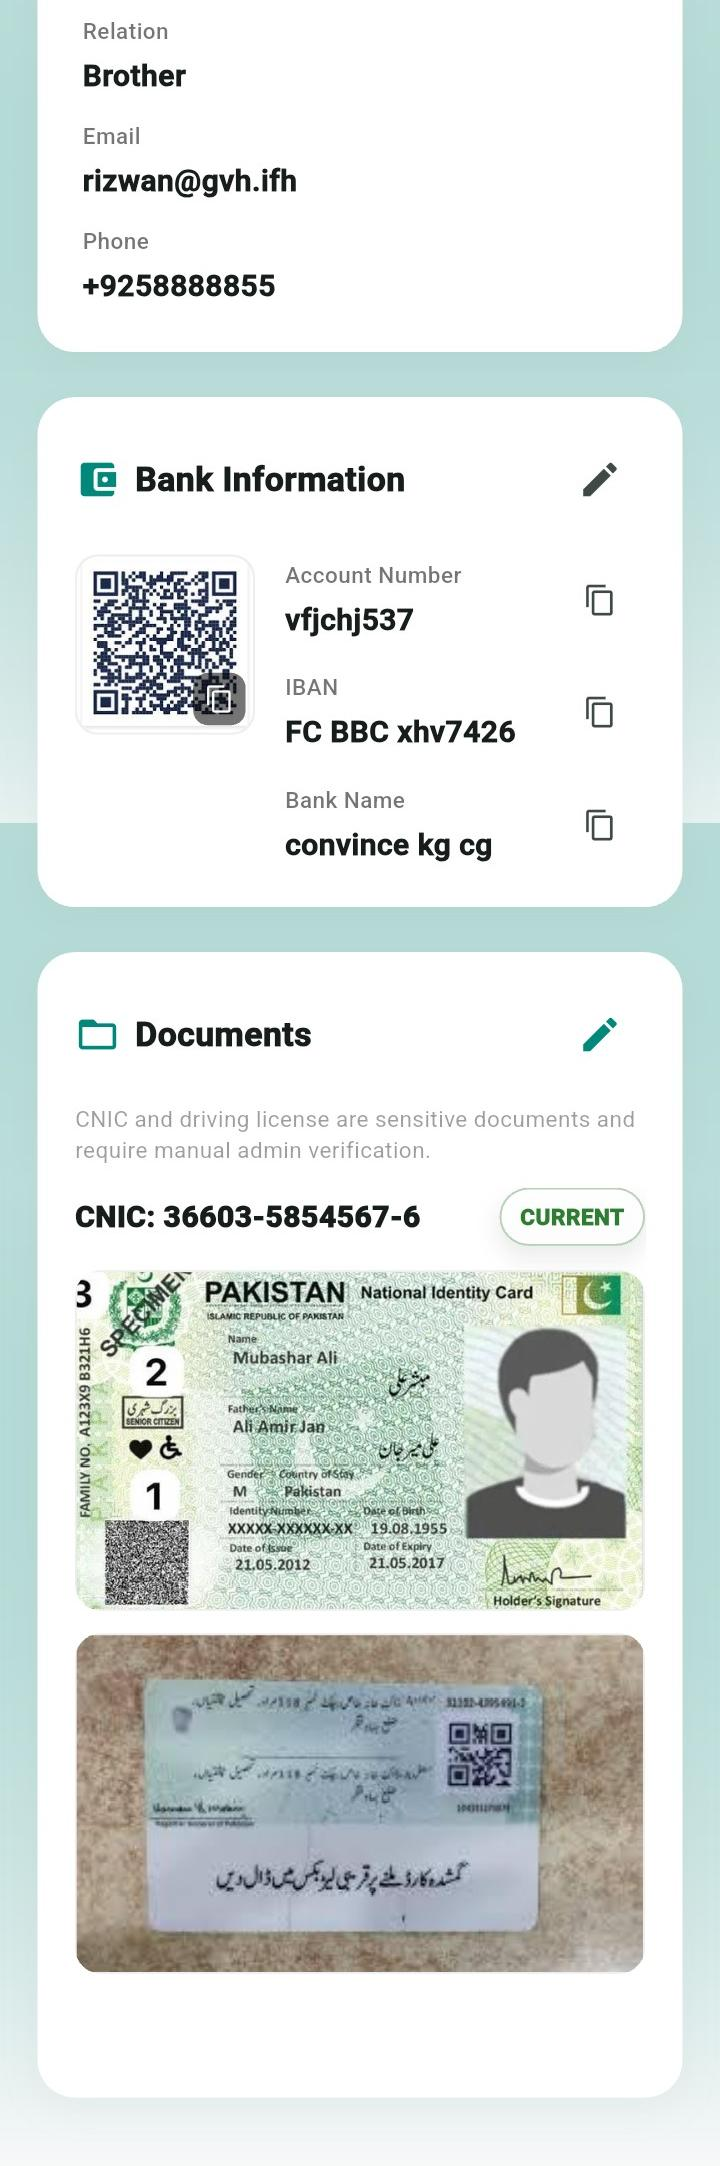
\includegraphics[width=\textwidth,height=0.8\textheight,keepaspectratio]{assets/app screenshot/profile_general_info_part2.jpeg}}
\end{minipage}
\caption{Profile Overview}
\end{figure}

Functional Flow: User accesses profile information, and accesses other linked areas like analytics, ride history, blocked users. Profile actions update the local state and instantaneously after successful backend updates.

\textbf{Backend Integration:} Profile data is retrieved from user profile endpoints and updated (e.g., edited) by authenticated API calls.

\textbf{Validation/Security:} edit must be authenticated, input validated before submission, and role checks for driver-only settings.

\subsubsection{Screen 37: Profile Analytics}

Purpose: Gives the user a combined overview of their riding history in the past.

Description: The screen includes time-based filtering (All-time, last 30 days, last 7 days) and provides key indicators for both driver and passenger positions. It provides a summary of created/booked rides, completion rates, distance covered and spending/revenue. Trend charts are used to show revenue and expenditures over time and a note box alerts the reader to possible data delays.

\begin{figure}[H]
\centering
\begin{minipage}{0.45\textwidth}
\centering
\fbox{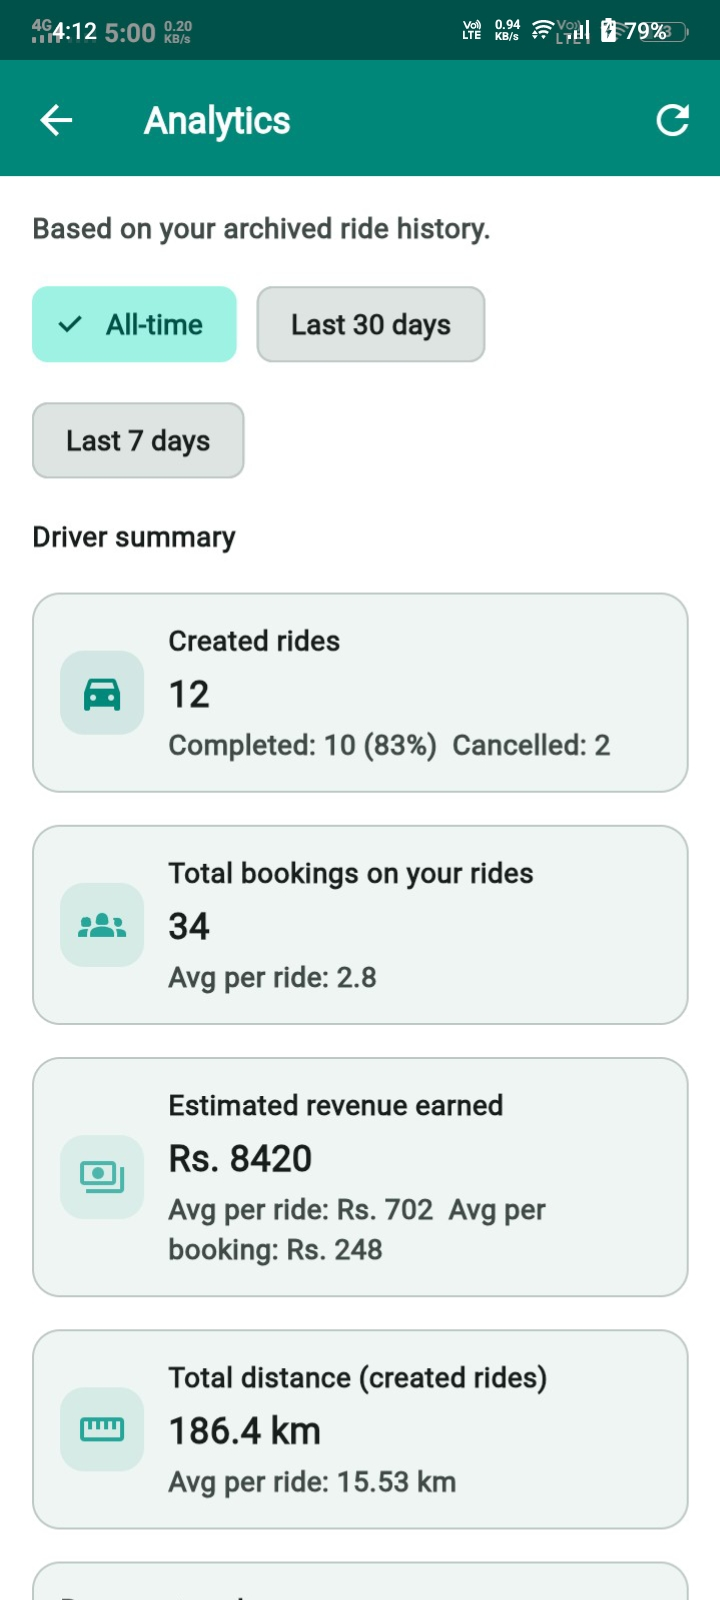
\includegraphics[width=\textwidth,height=0.6\textheight,keepaspectratio]{assets/app screenshot/analytics_part_1.jpeg}}
\end{minipage}\hfill
\begin{minipage}{0.45\textwidth}
\centering
\fbox{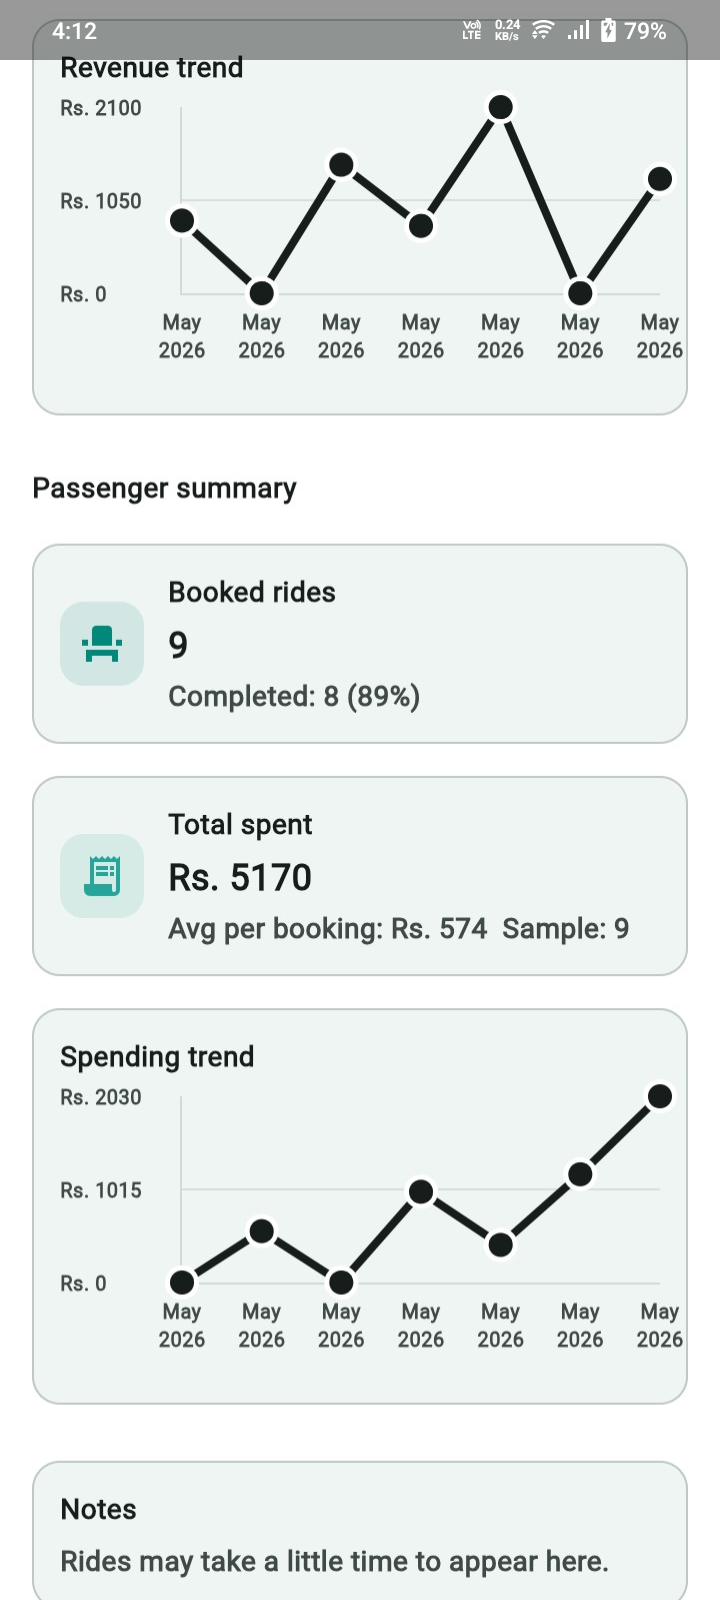
\includegraphics[width=\textwidth,height=0.6\textheight,keepaspectratio]{assets/app screenshot/analytics_part_2.jpeg}}
\end{minipage}
\caption{Profile Analytics}
\end{figure}

\subsubsection{Screen 38: Ride History (Booked/Created)}

Use for: Accessing and reviewing previous trip information.

\textbf{Components:}
\begin{itemize}
    \item History records with details of the routes.
\end{itemize}

\begin{figure}[H]
\centering
\begin{minipage}{0.45\textwidth}
\centering
\fbox{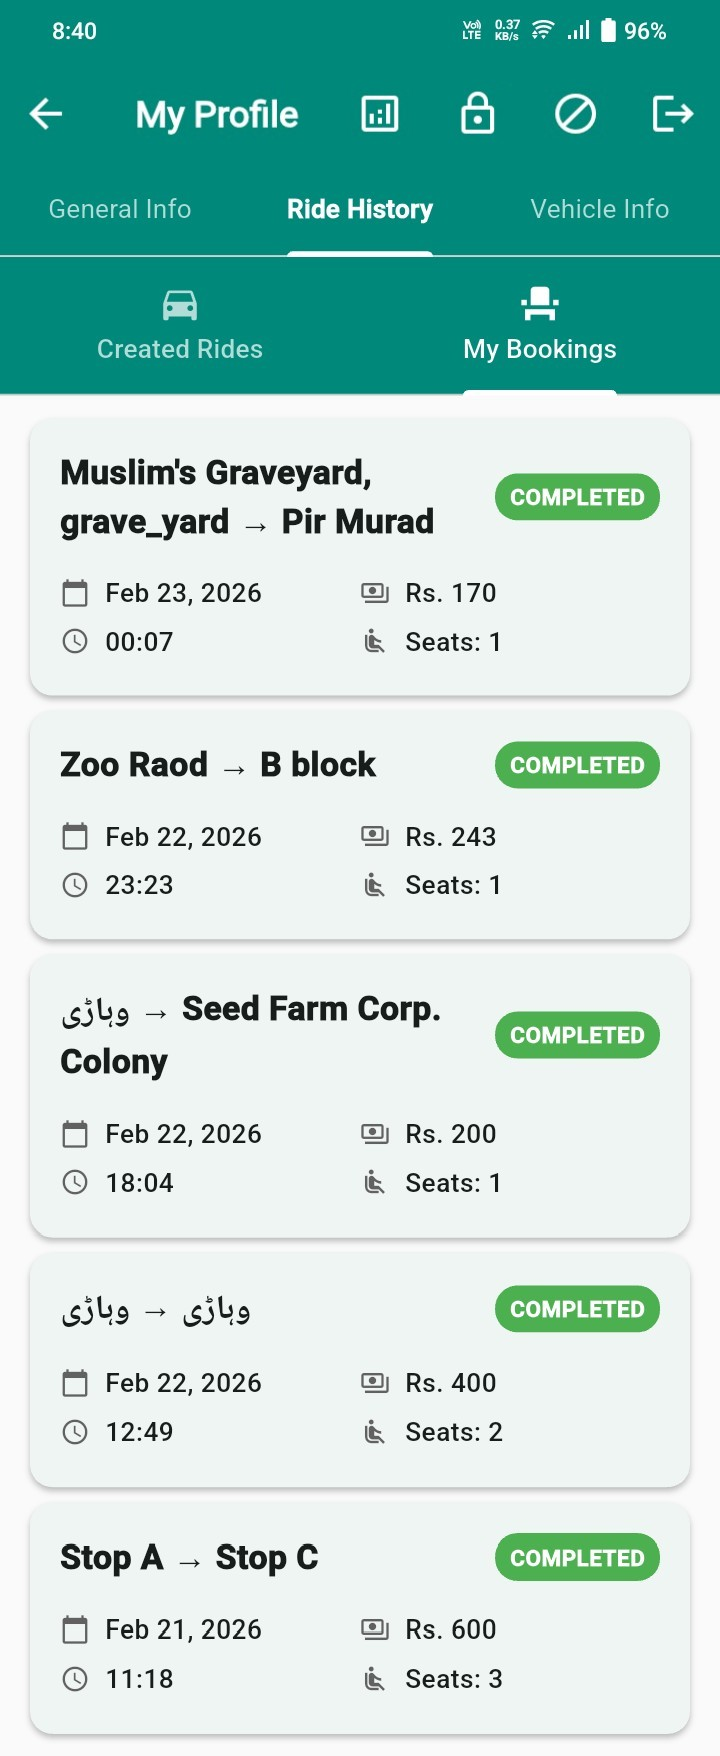
\includegraphics[width=\textwidth,keepaspectratio]{assets/app screenshot/profile_booked_ride_history.jpeg}}
\end{minipage}\hfill
\begin{minipage}{0.45\textwidth}
\centering
\fbox{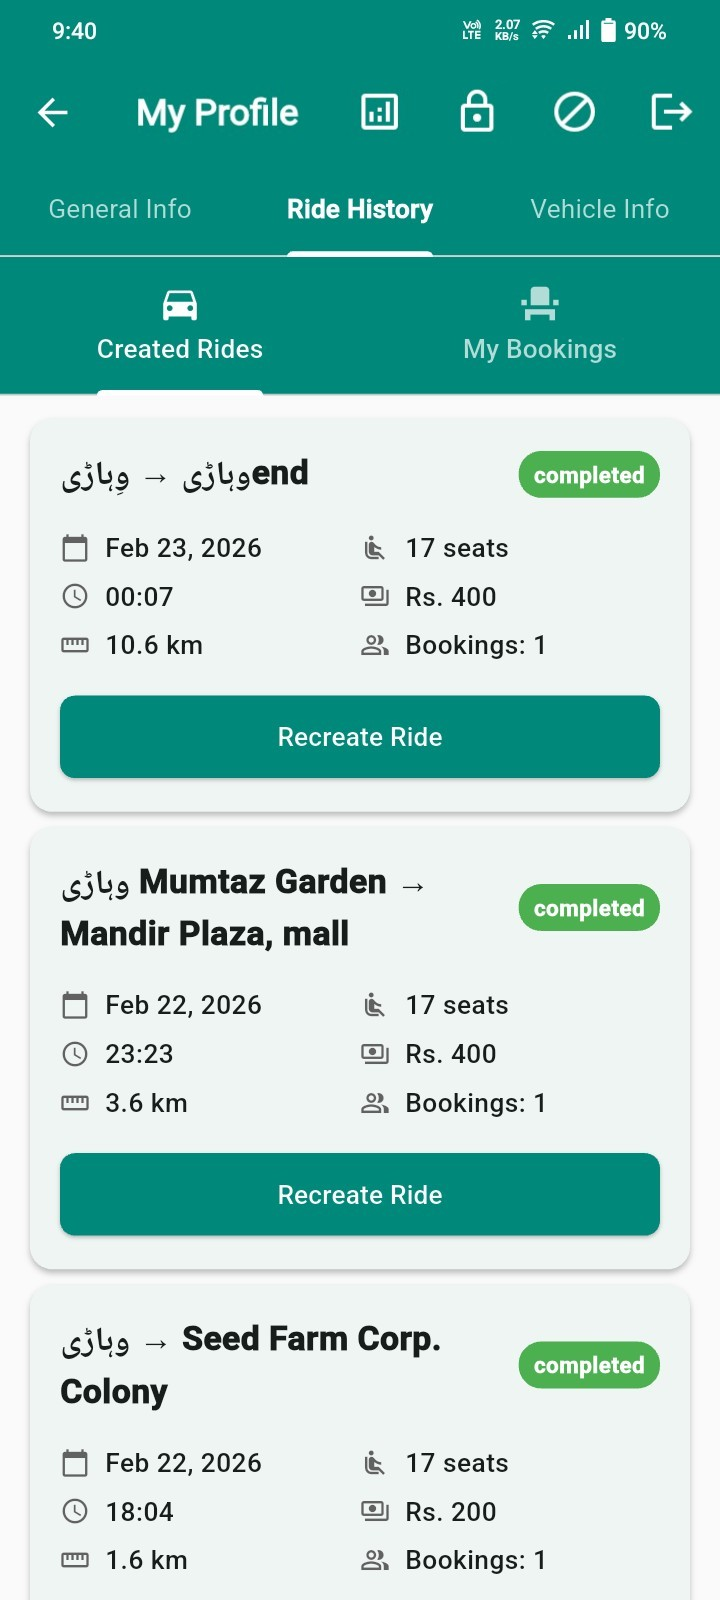
\includegraphics[width=\textwidth,keepaspectratio]{assets/app screenshot/profile_created_rides_history.jpeg}}
\end{minipage}
\caption{Ride History (Booked/Created)}
\end{figure}

Functional Flow: User scrolls through rides and views key ride information (route summary, status). Clicking on an item can trigger more detailed views, based on role and availability.

Backend integration: Ride history is loaded from booking/trip history endpoints, including pagination for large histories.

Validation/Security: Data from history is only accessible to the owner account and details of passengers/drivers is kept to a minimum in list views.

\subsubsection{Screen 39: Driver Verification Documents (Edit)}

Use this screen to edit the driver verification documents.This screen is used for editing the driver verification documents.

The purpose of this document is to provide a portal for keeping drivers and vehicles eligible.

\textbf{Components:}
Uploading images and inputting ID and vehicle registration.

\begin{figure}[H]
\centering
\begin{minipage}{0.30\textwidth}
\centering
\fbox{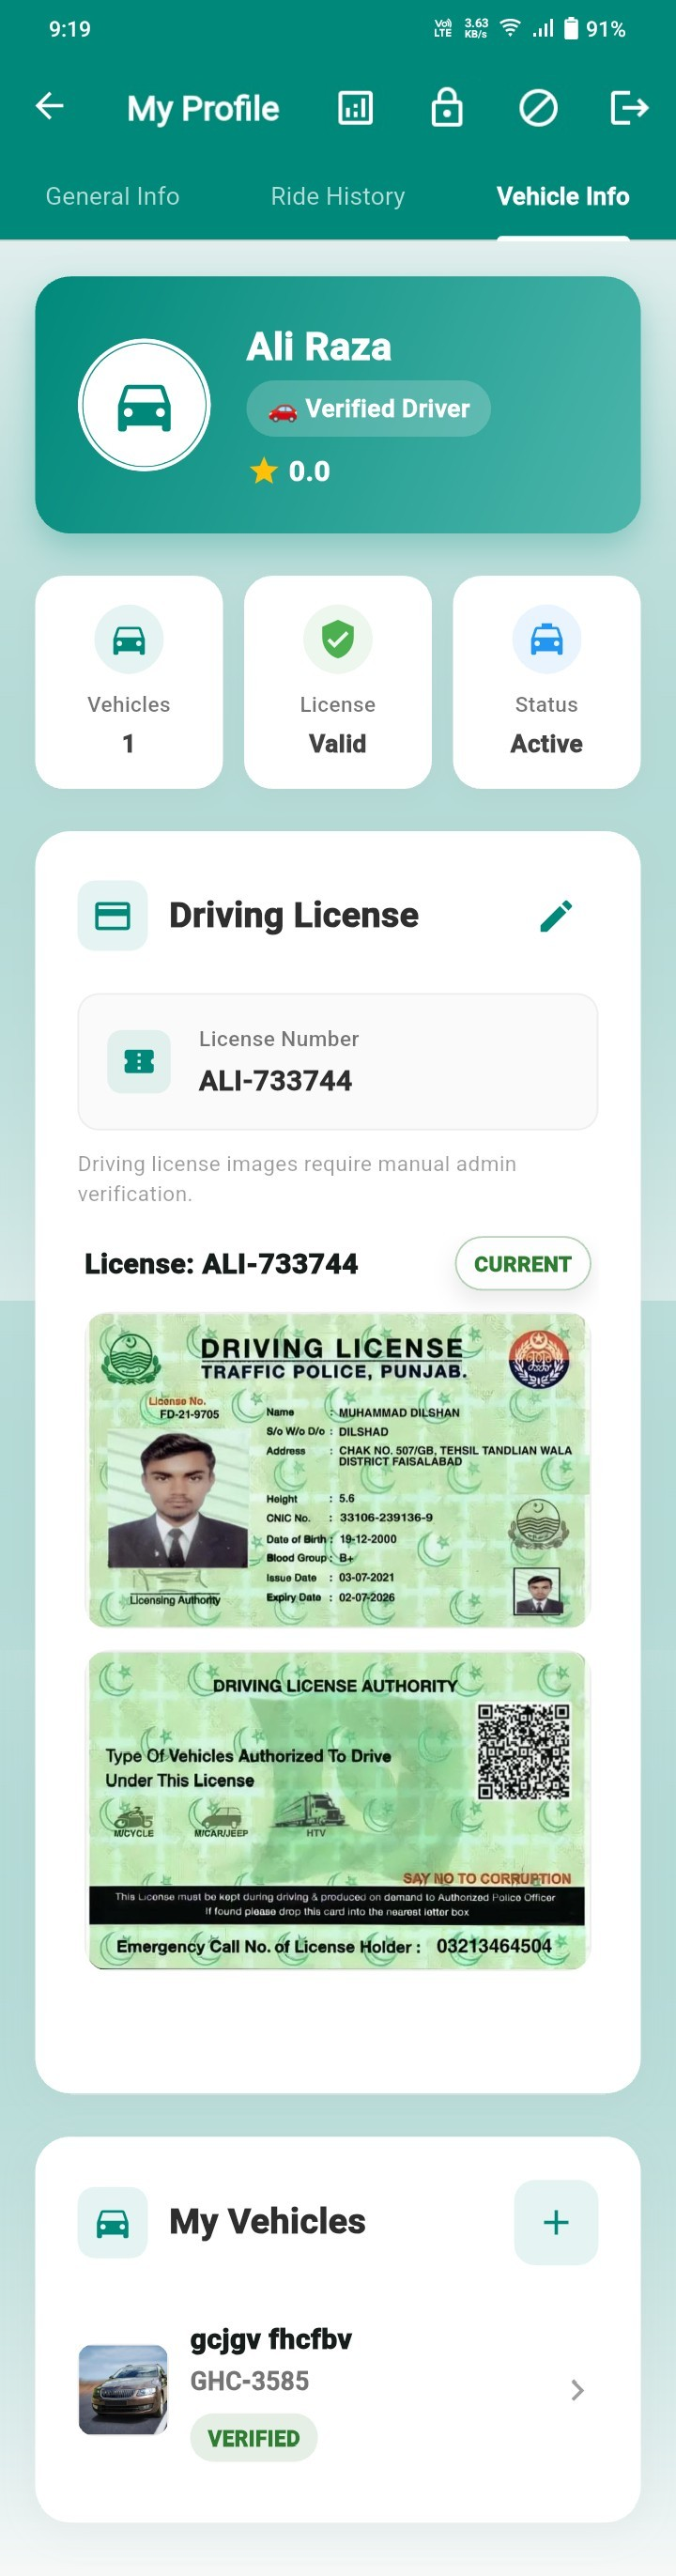
\includegraphics[width=\textwidth,height=0.55\textheight,keepaspectratio]{assets/app screenshot/driver_license_vehicle_info.jpeg}}
\end{minipage}\hfill
\begin{minipage}{0.30\textwidth}
\centering
\fbox{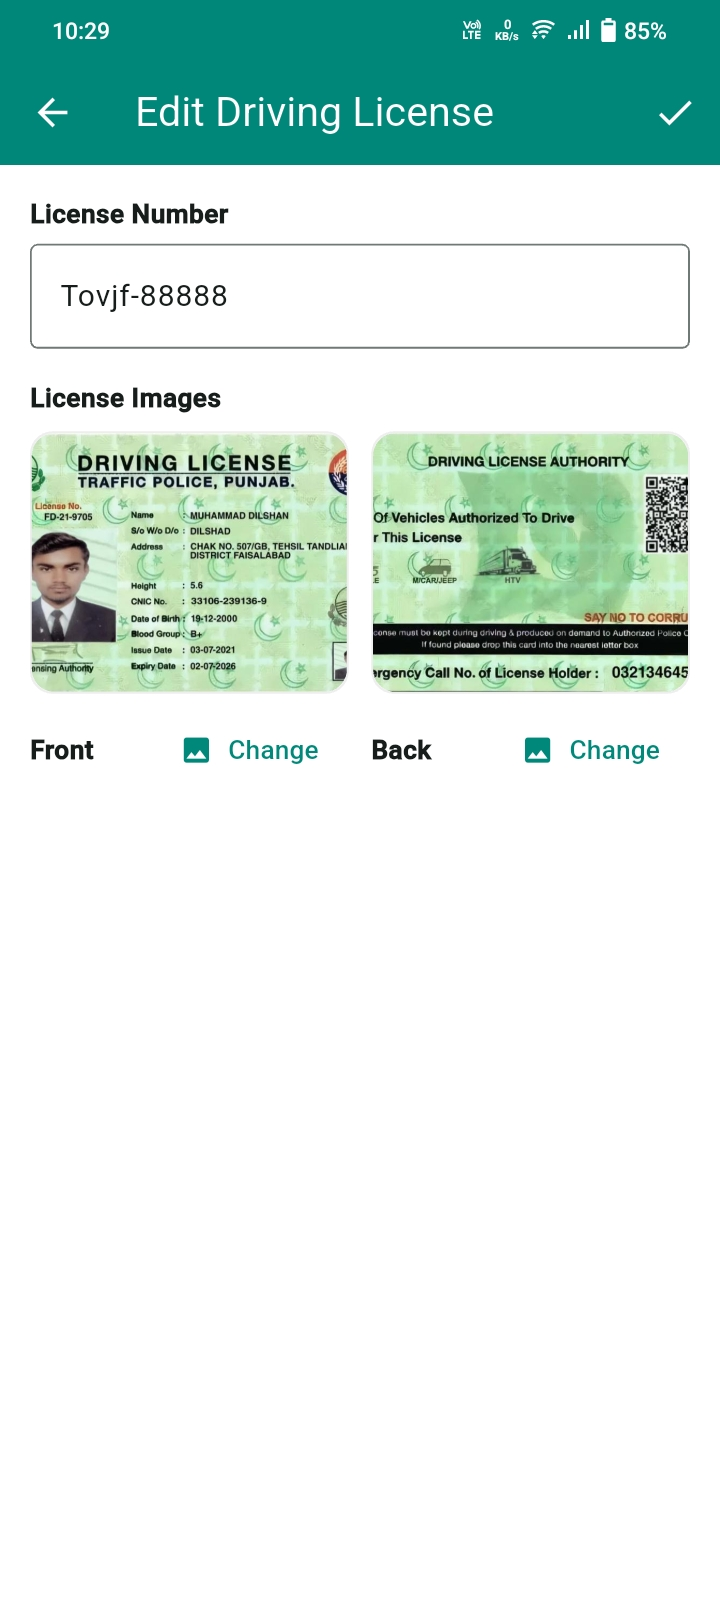
\includegraphics[width=\textwidth,keepaspectratio]{assets/app screenshot/edit_driving_license.jpeg}}
\end{minipage}\hfill
\begin{minipage}{0.30\textwidth}
\centering
\fbox{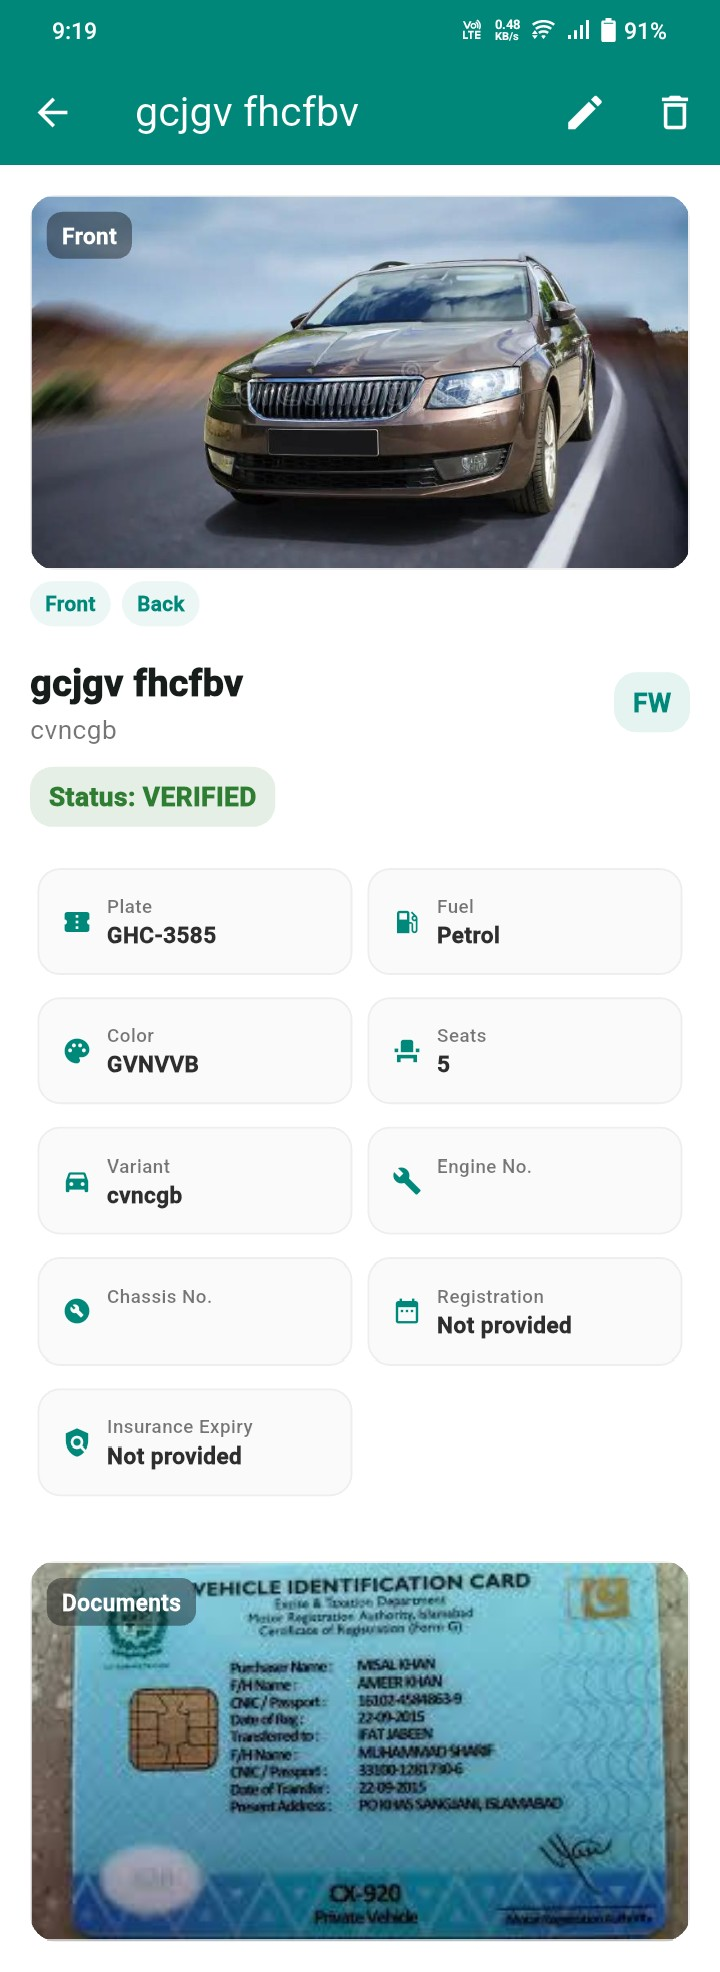
\includegraphics[width=\textwidth,keepaspectratio]{assets/app screenshot/vehicle_details_card.jpeg}}
\end{minipage}
\caption{Driver Verification Documents (Edit)}
\end{figure}

Functional Flow: Drivers upload and/or update their license and vehicle documents and submit them for verification. The UI gives instant feedback and driver eligibility is based on the verification status.

\textbf{Backend Integration:} Document metadata and images are uploaded to the backend storage layer, and are correlated with the driver profile for Admin review.

\textbf{Validation/Security:} File types and sizes are validated, uploads must be authenticated and documents are only accessible to authorised roles.

\subsubsection{Screen 40: Blocked Users}

Purpose: Users can use the blocked accounts functionality to limit their interactions on the platform.

\textbf{Components:}
\begin{itemize}
    \item Blocked user list and user search/filter controls.
\end{itemize}

\begin{figure}[H]
\centering
\fbox{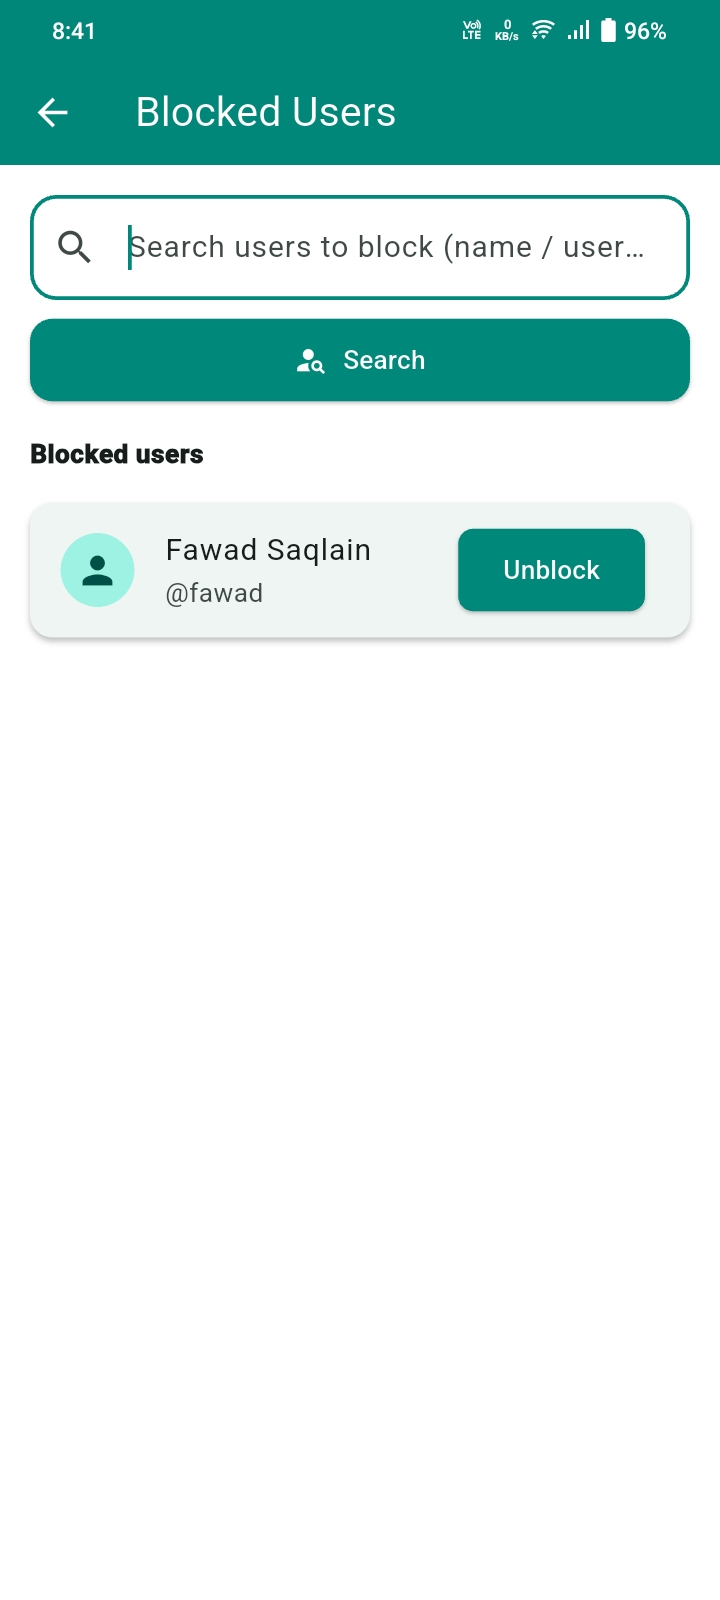
\includegraphics[width=\textwidth,height=0.6\textheight,keepaspectratio]{assets/app screenshot/blocked_users_list.jpeg}}
\caption{Blocked Users}
\end{figure}

Functional Flow: User will see blocked accounts and will be able to unblock users to re-enable interaction. After a block/unblock operation, the list will be updated immediately.

Backend Integration: Block/Unblock actions are saved through profile privacy endpoints and are synced with access to chat and/or search.

Validation/Security: Blocking is done on the server side to prevent unwanted contact in the messaging and booking flow.

\subsubsection{Screen 41: Web Live Tracking (External)}

Web Live Tracking (External): Screen 41

\textbf{Target:} A person with access to a desktop computer.\textbf{Goal:} Enable a person to track their ride using a desktop computer.

\textbf{Components:}
Real time map and trip status for the desktop.

\begin{figure}[H]
\centering
\fbox{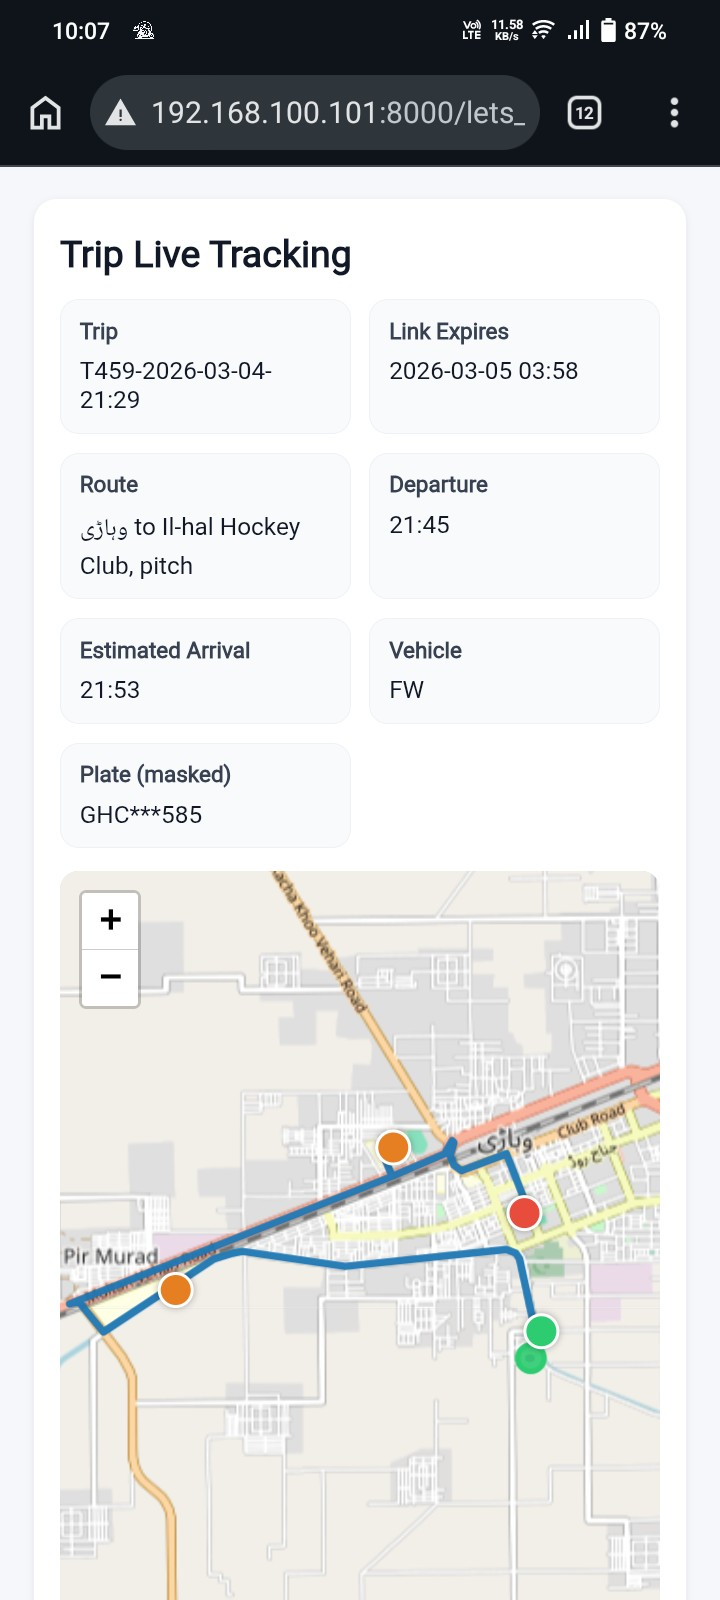
\includegraphics[width=\textwidth,keepaspectratio,height=0.6\textheight]{assets/app screenshot/web_live_tracking.jpeg}}
\caption{Web Live Tracking (External)}
\end{figure}

Functional Flow: The user accesses a web-based tracking view to see more of a trip on a larger screen. Active route and status are indicated on the map which is updated regularly.

Backend Integration: View subscribes to tracking endpoints for current location snapshots and tracking status changes.

Validation/Security: Data is shared only with authorised viewers (trip participants or Admin) and share links are validated before displaying data.

\textbf{Admin Module Overview:} Administrative web dashboards for monitoring rides, users, SOS incident, operational requests etc. are available in the administration module for authenticated users. Backend templates are used to serve all admin pages and role-based authorization is used to protect these pages.

\subsubsection{Screen 42: Admin Login}
Authorizes entry point for Admin authentication and session creation.

Components: Login form, error feedback and session/redirect handling.

Functional Flow: Admin provides credentials and receives authenticated session to access a protected dashboard.

Backend Integration: Administration login view and Session middleware.

\textbf{Validation/Security:} Server-side validation and access to dashboards is denied without a valid Admin session.

\begin{figure}[H]
\centering
\fbox{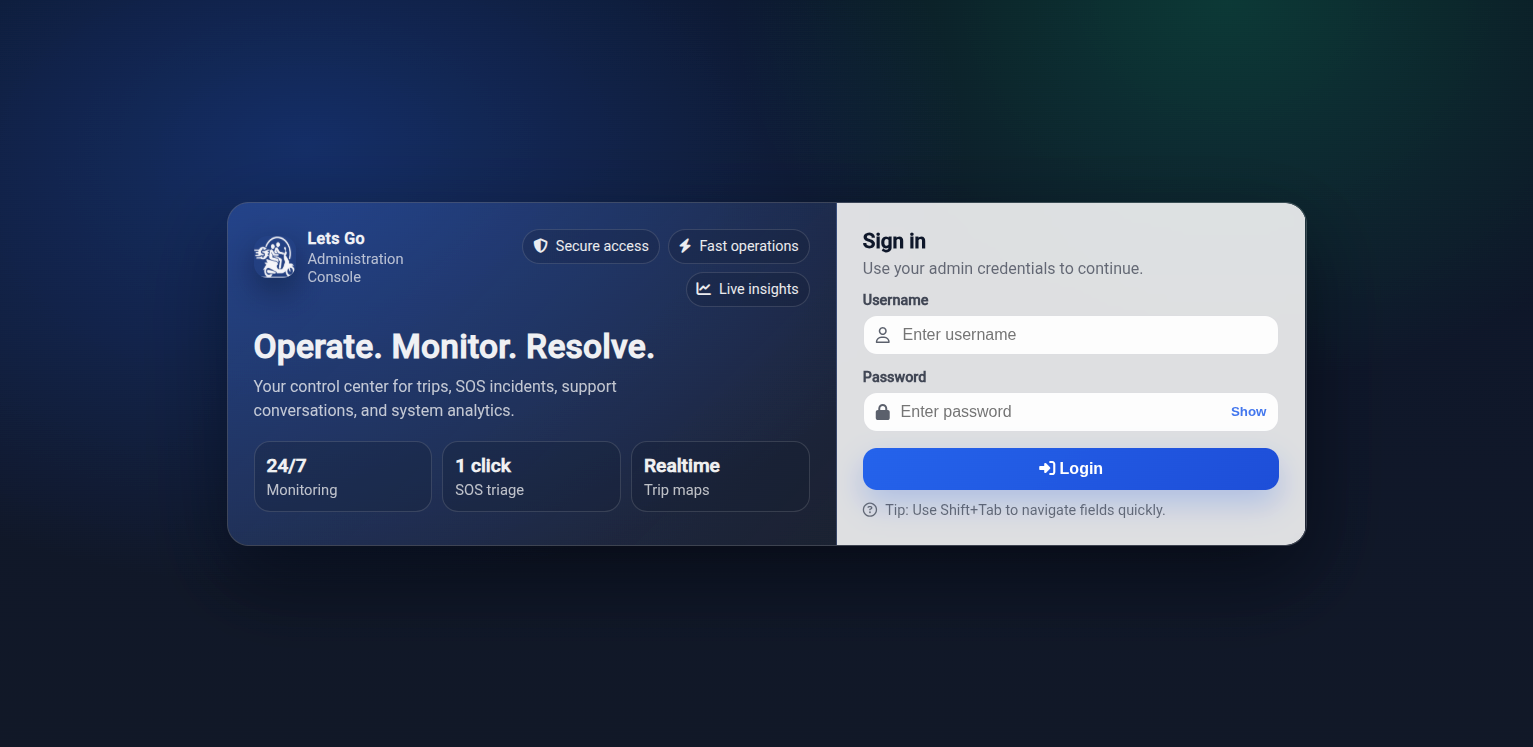
\includegraphics[width=0.85\textwidth,keepaspectratio]{assets/app screenshot/dashboard images/administration-login.png}}
\caption{Admin Login Screen}
\end{figure}

\subsubsection{Screen 43: Admin Dashboard (Overview)}
Purpose: High level view of platform health and important operational counters.

Components: Summary cards, quick links and key metric widgets.

Functional Flow: Fills summary cards and connects to more detailed dashboards like SOS and reached pending.

Backend Integration: Integrates ride, user and incident data from the administration dashboard view.

Validation/Security: Metrics are based on trusted data sources and displayed only to approved Admin roles.

\begin{figure}[H]
\centering
\fbox{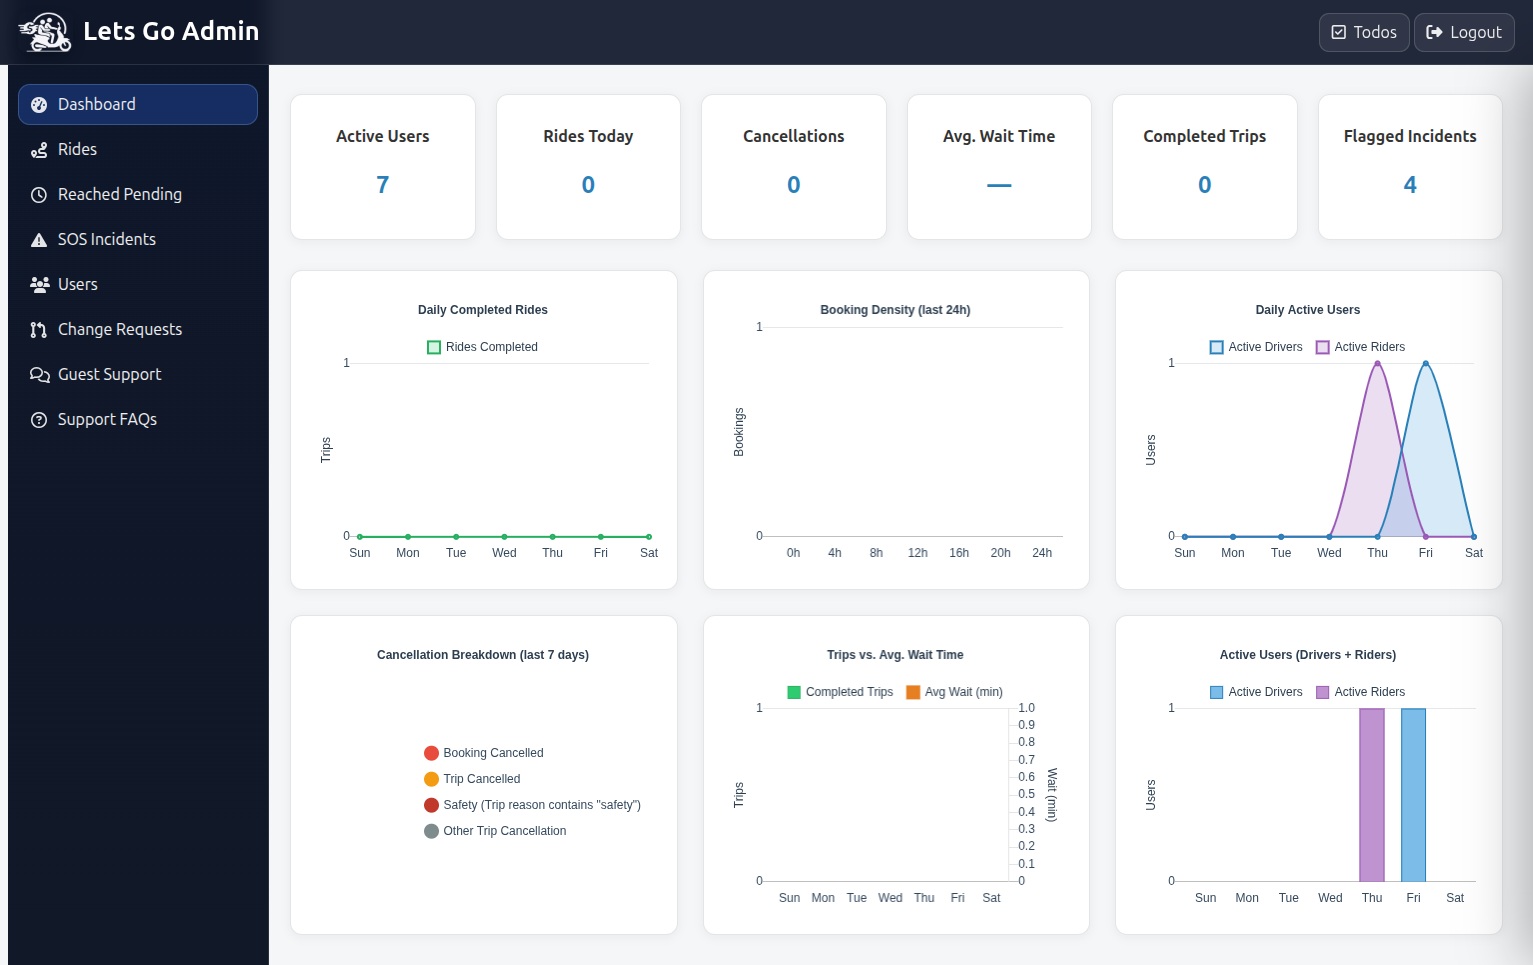
\includegraphics[width=0.85\textwidth,keepaspectratio]{assets/app screenshot/dashboard images/administration-dashboard.png}}
\caption{Admin Dashboard (Overview)}
\end{figure}

\subsubsection{Screen 44: Rides Dashboard}
\textbf{Description:} Watch published rides and ride lifecycle data.

Ride listing table, filters and navigation to ride/trip detail pages.

Functional Flow: Admin filters and views rides and opens trip detail pages to investigate rides.

Backend Integration: Provided through rides dashboard template and corresponding Django view.

Validation/Security: Only admin users have access to the admin area, and sensitive fields are not visible to non-admin users.

\begin{figure}[H]
\centering
\fbox{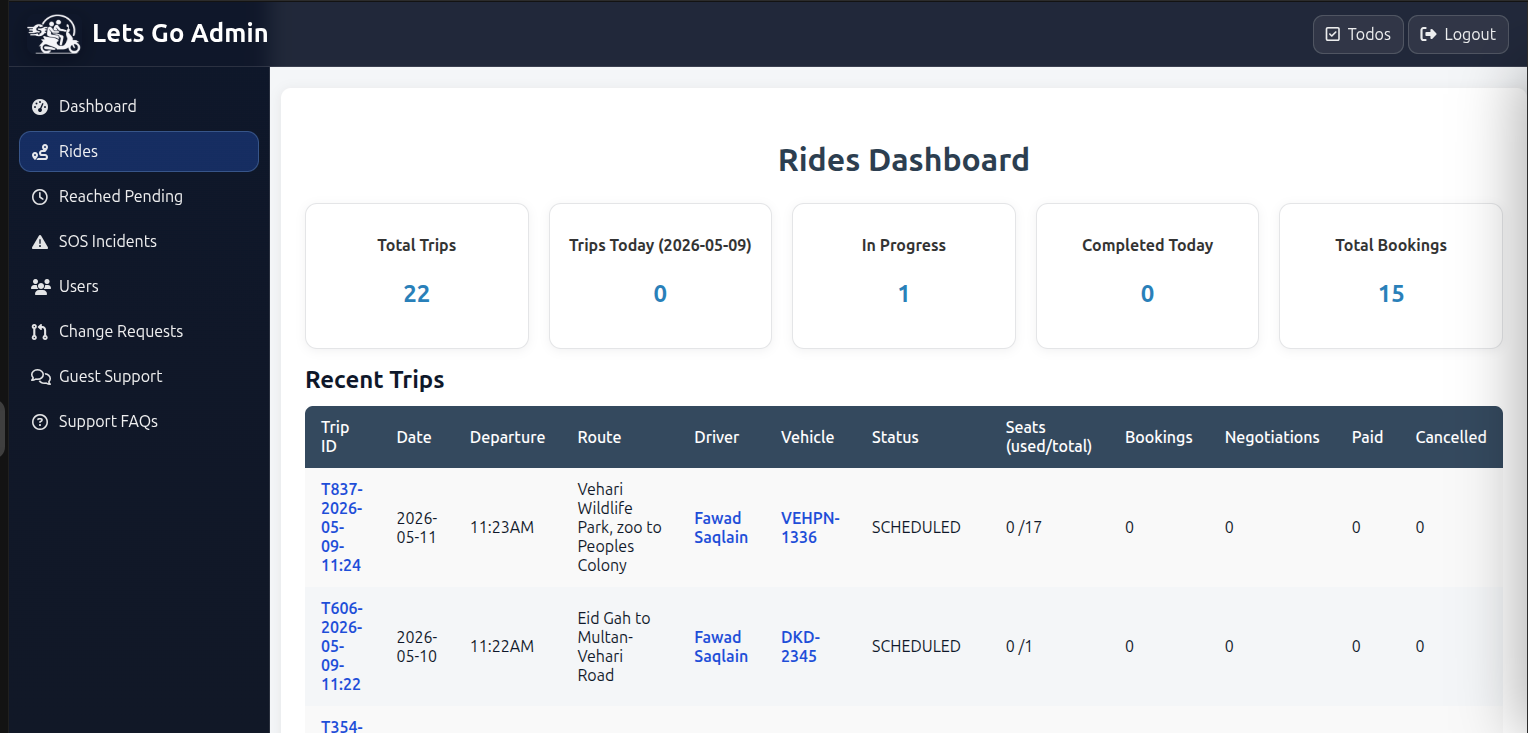
\includegraphics[width=0.85\textwidth,keepaspectratio]{assets/app screenshot/dashboard images/Rides-Dashboard.png}}
\caption{Rides Dashboard}
\end{figure}

\subsubsection{Screen 45: Reached Pending Dashboard}
Purpose: Identify riders who have reached/overdue status that needs follow-up.

The components are the pending/overdue list, status indicators and navigation controls.

Functional Flow: Admin reviews overdue entries and moves on to detail screens for action.

Backend Integration: With reached overdue dashboard view and template.

Validation/Security: List is created from verified ride states and only accessible in authenticated Admin sessions.

\begin{figure}[H]
\centering
\fbox{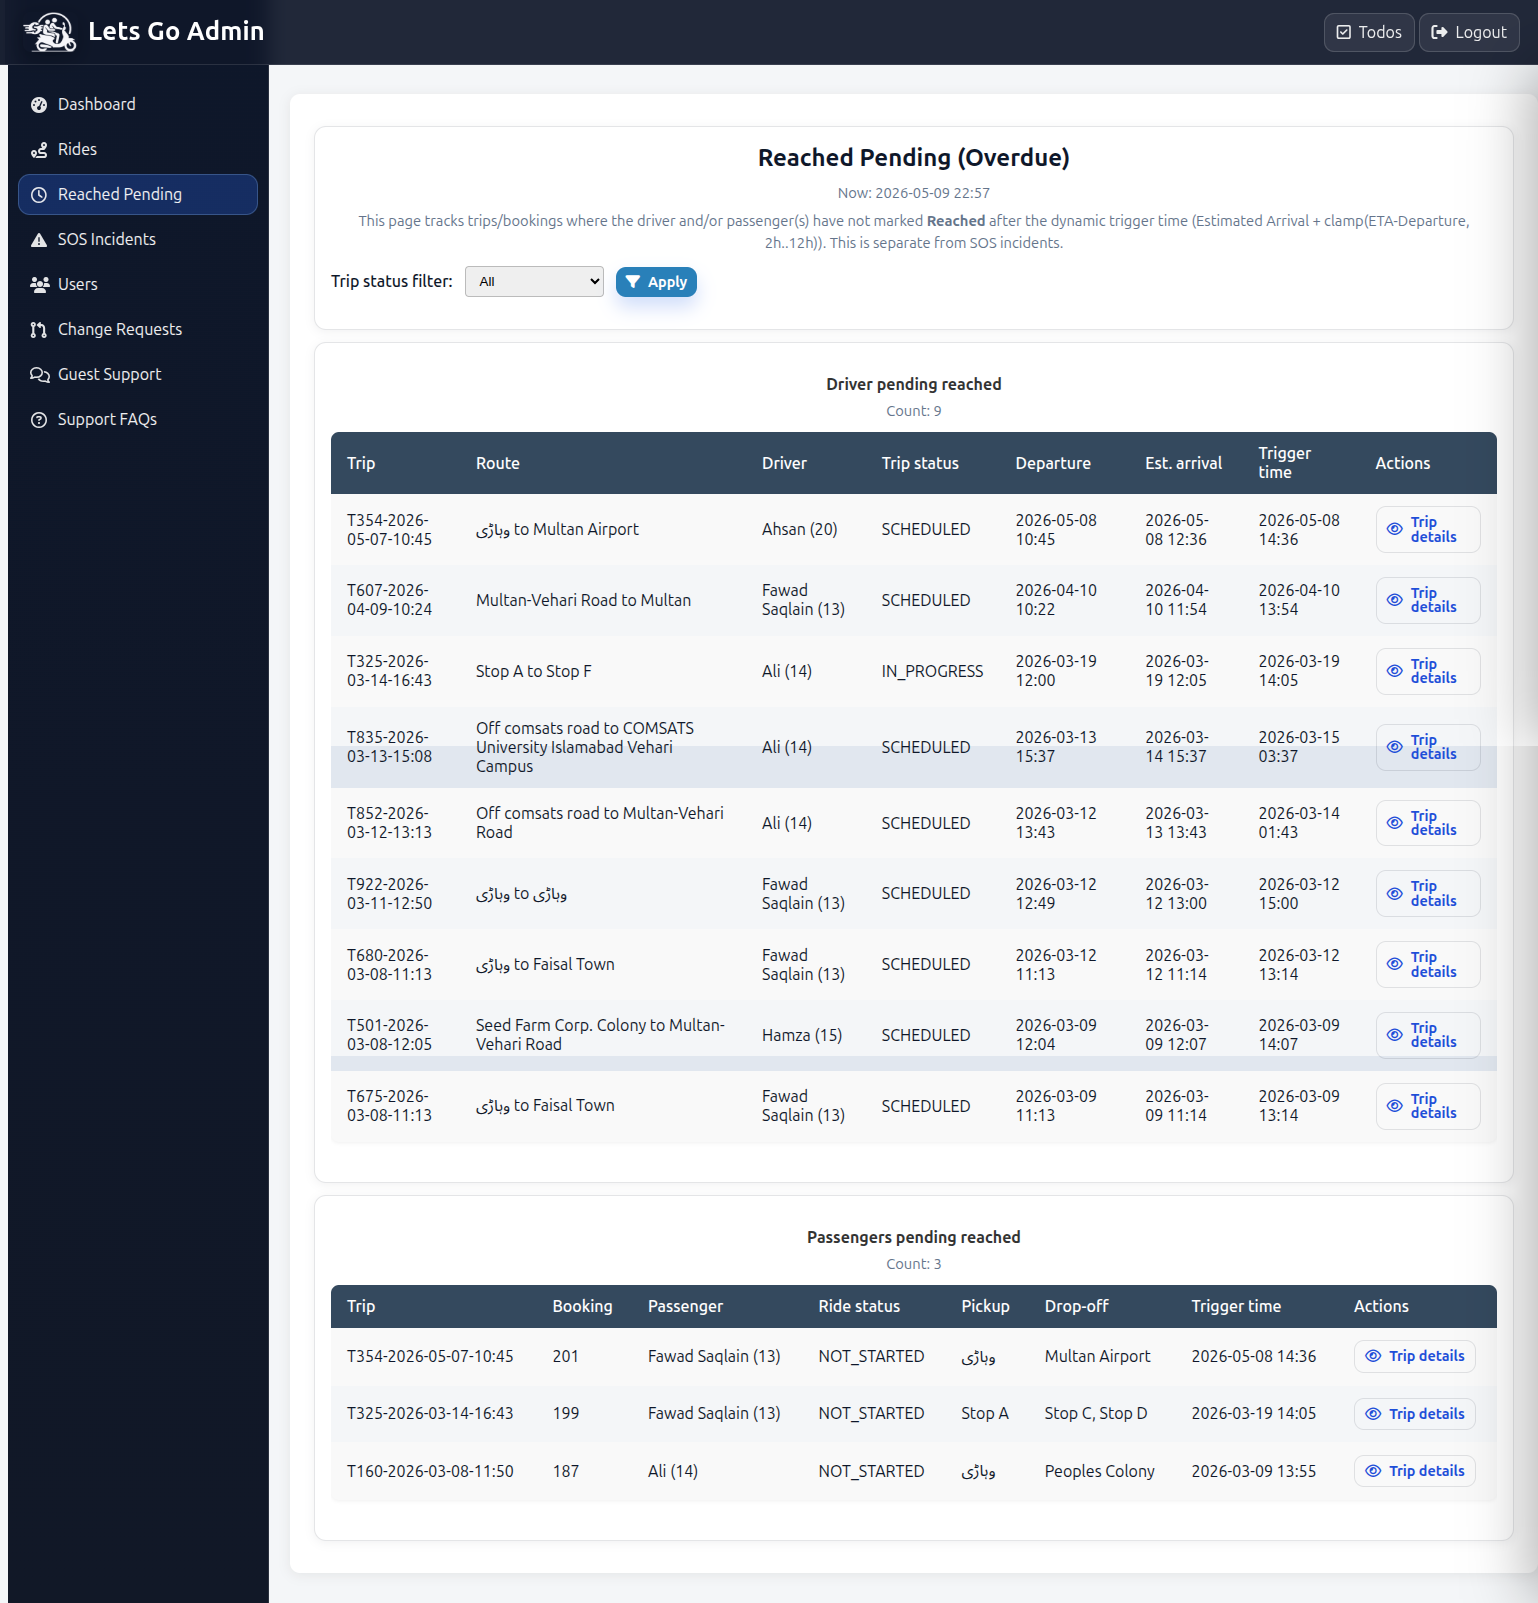
\includegraphics[width=0.85\textwidth,keepaspectratio]{assets/app screenshot/dashboard images/administration-reached.png}}
\caption{Reached Pending Dashboard}
\end{figure}

\subsubsection{Screen 46: SOS Incidents Dashboard}
Safety Monitoring Dashboard for reviewing, reacting to and resolving SOS incidents.

Components: Incident table, incident detail navigation, resolution/Status controls.

Admin opens an incident, reads through the location and metadata, and checks it off when action is taken.

Backend Integration: Backend dashboards and incident detail views served from Django templates.

Security/Validation: Access to incidents is role-restricted, and all state changes are done server side.

\begin{figure}[H]
\centering
\fbox{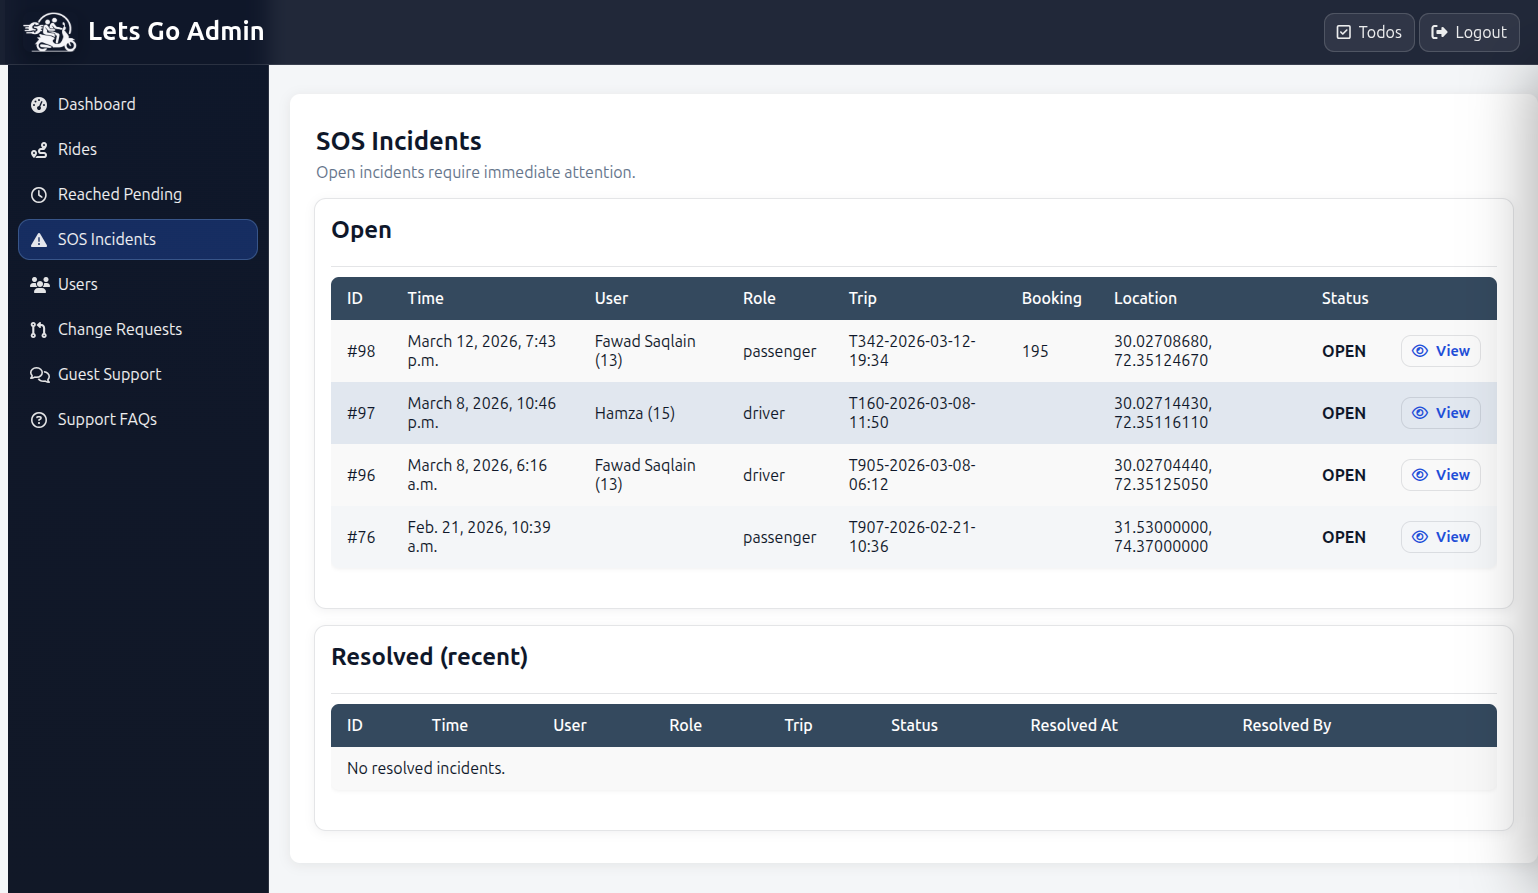
\includegraphics[width=0.85\textwidth,keepaspectratio]{assets/app screenshot/dashboard images/administration-sos.png}}
\caption{SOS Incidents Dashboard}
\end{figure}

\subsubsection{Screen 47: Users Management}
Purpose: to control the user accounts, to check the status, and to help with moderation processes.

Features include user list/search, detail views and administrative action controls.

Functional Flow: Admin searches users, opens details, and does allowed actions according to the policy.

Backend Integration: Loaded in User list/detail views in the admin module.

Validation/Security: Server-side validation of actions and only for Admin roles.

\begin{figure}[H]
\centering
\fbox{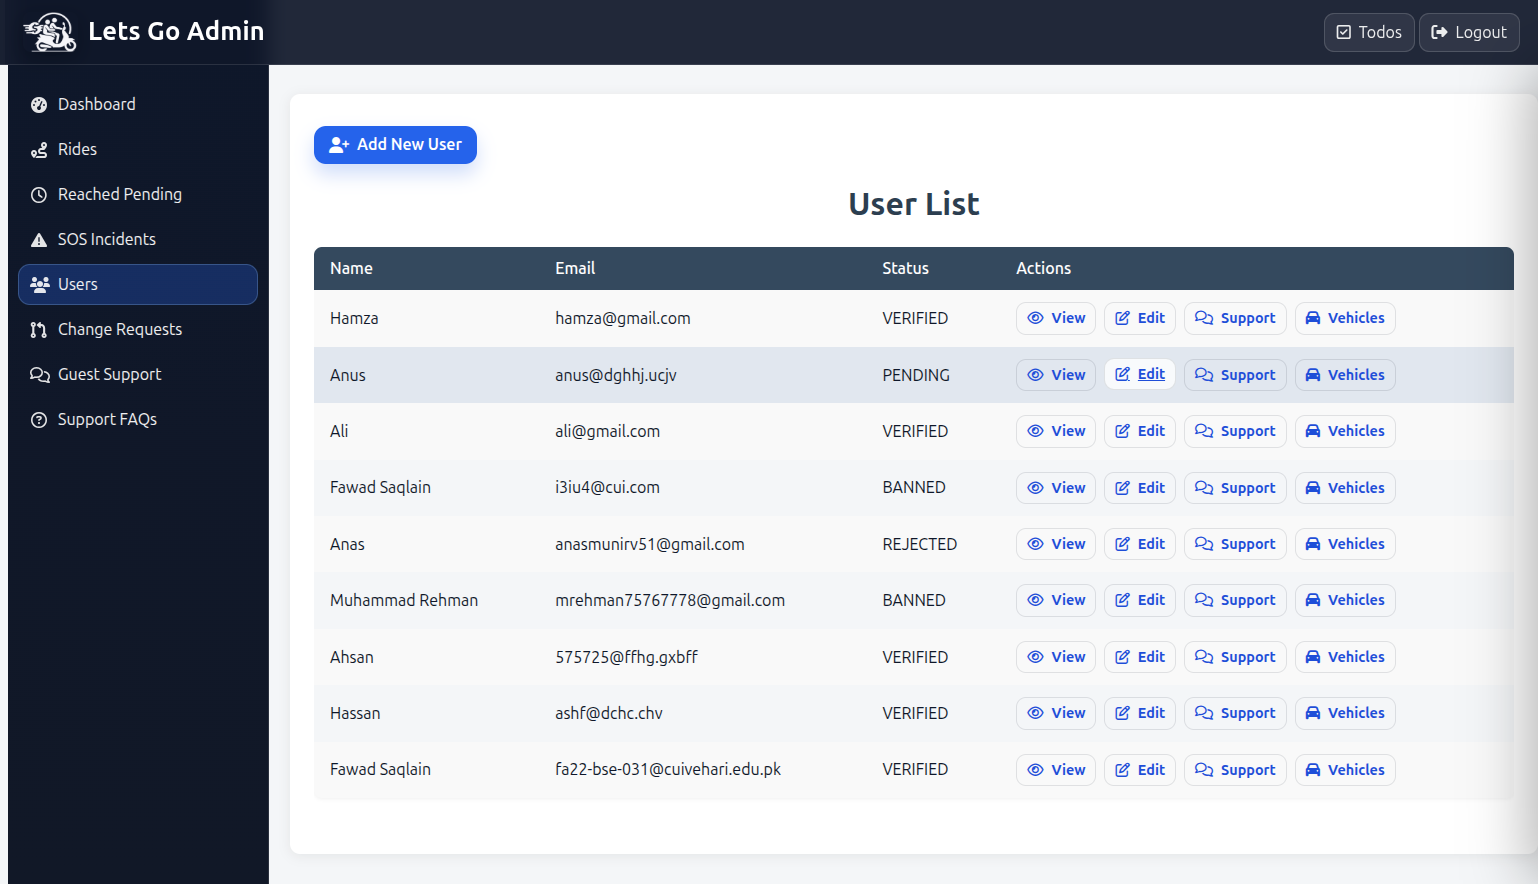
\includegraphics[width=0.85\textwidth,keepaspectratio]{assets/app screenshot/dashboard images/administration-users.png}}
\caption{Users Management Screen}
\end{figure}

\subsubsection{Screen 48: Change Requests Dashboard}
Use to monitor and log ride change requests from users.

The following components will be used: Request queue, request detail views, and approve and reject controls.

Functional Flow: Admin checks each request, and based on constraints he approves or rejects.

Backend Integration: Was provided through change request list/detail templates and views.

All requests are validated against ride constraints; any decisions are made server side (validation/security).

\begin{figure}[H]
\centering
\fbox{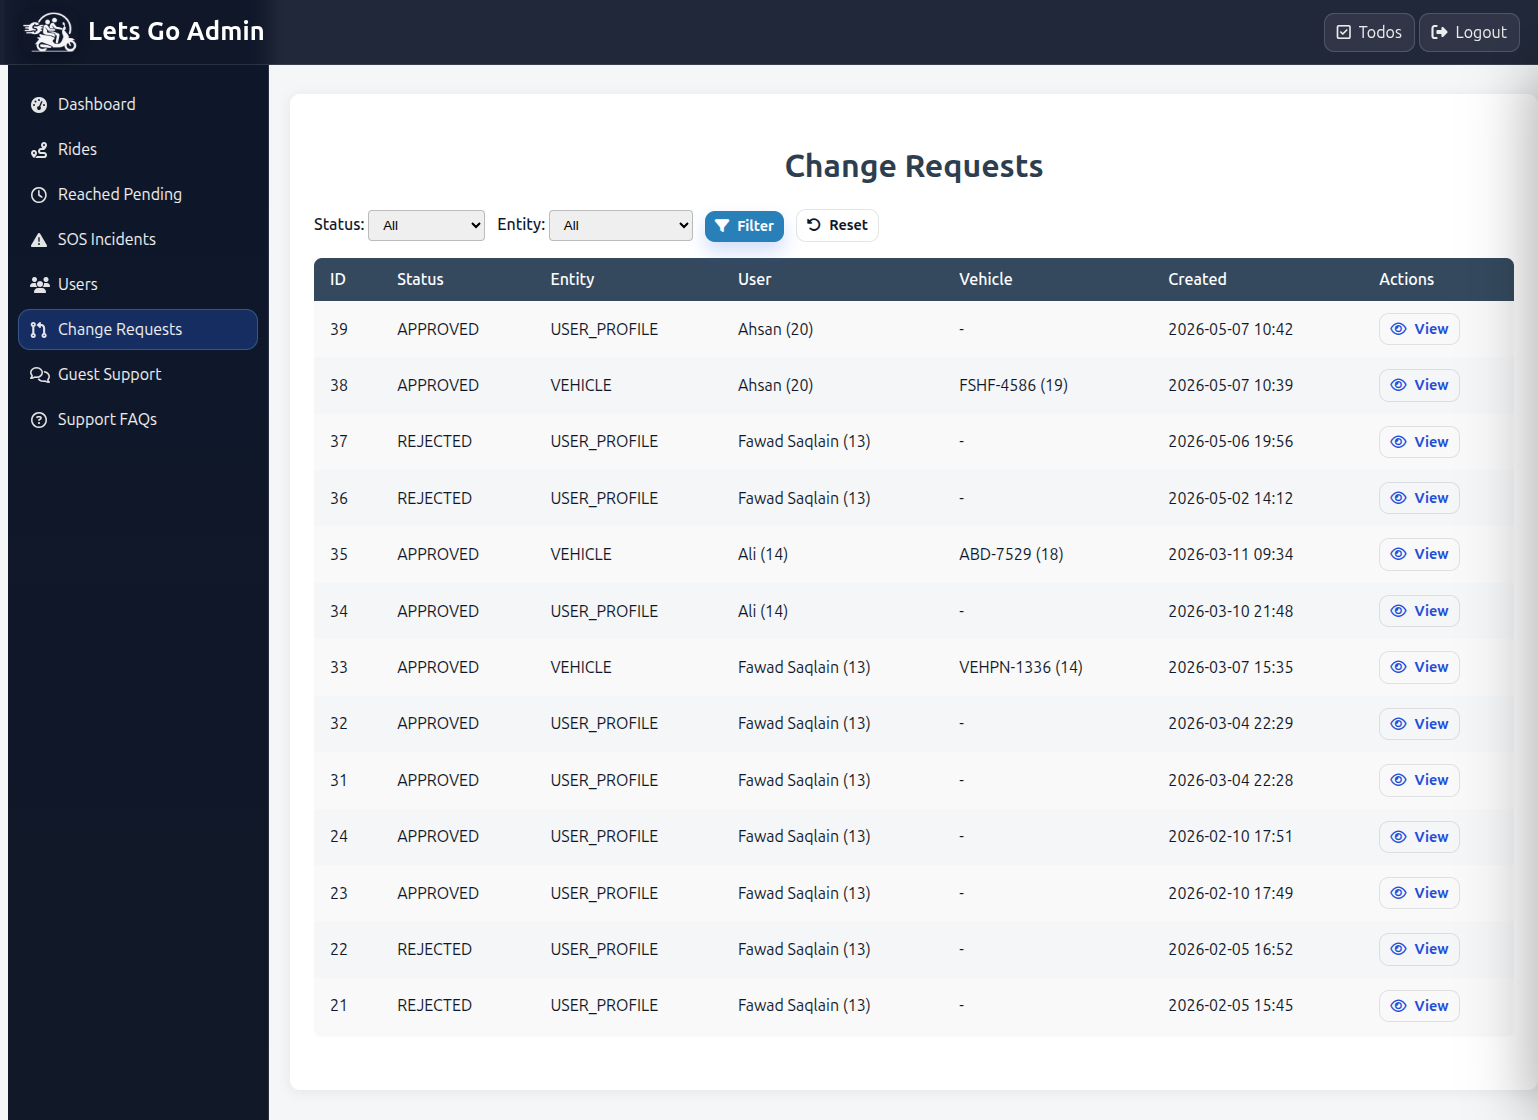
\includegraphics[width=0.85\textwidth,keepaspectratio]{assets/app screenshot/dashboard images/administration-change-requests.png}}
\caption{Change Requests Dashboard}
\end{figure}

\subsubsection{Screen 49: Admin Todos Inbox}
Purpose: Single source of information for tasks and follow-ups in operation.

Components: ToDo items and links to other entities, as well as task status indicators.

Functional Flow: Admin approves pending records and clicks on related entities to finish the job.

Back end integration: Embedded todos inbox view and supporting endpoints.

The following are also secured: Validation/Security: Todos can only be accessed by Admin sessions, updates to tasks are persisted using a secured endpoint.

\begin{figure}[H]
\centering
\fbox{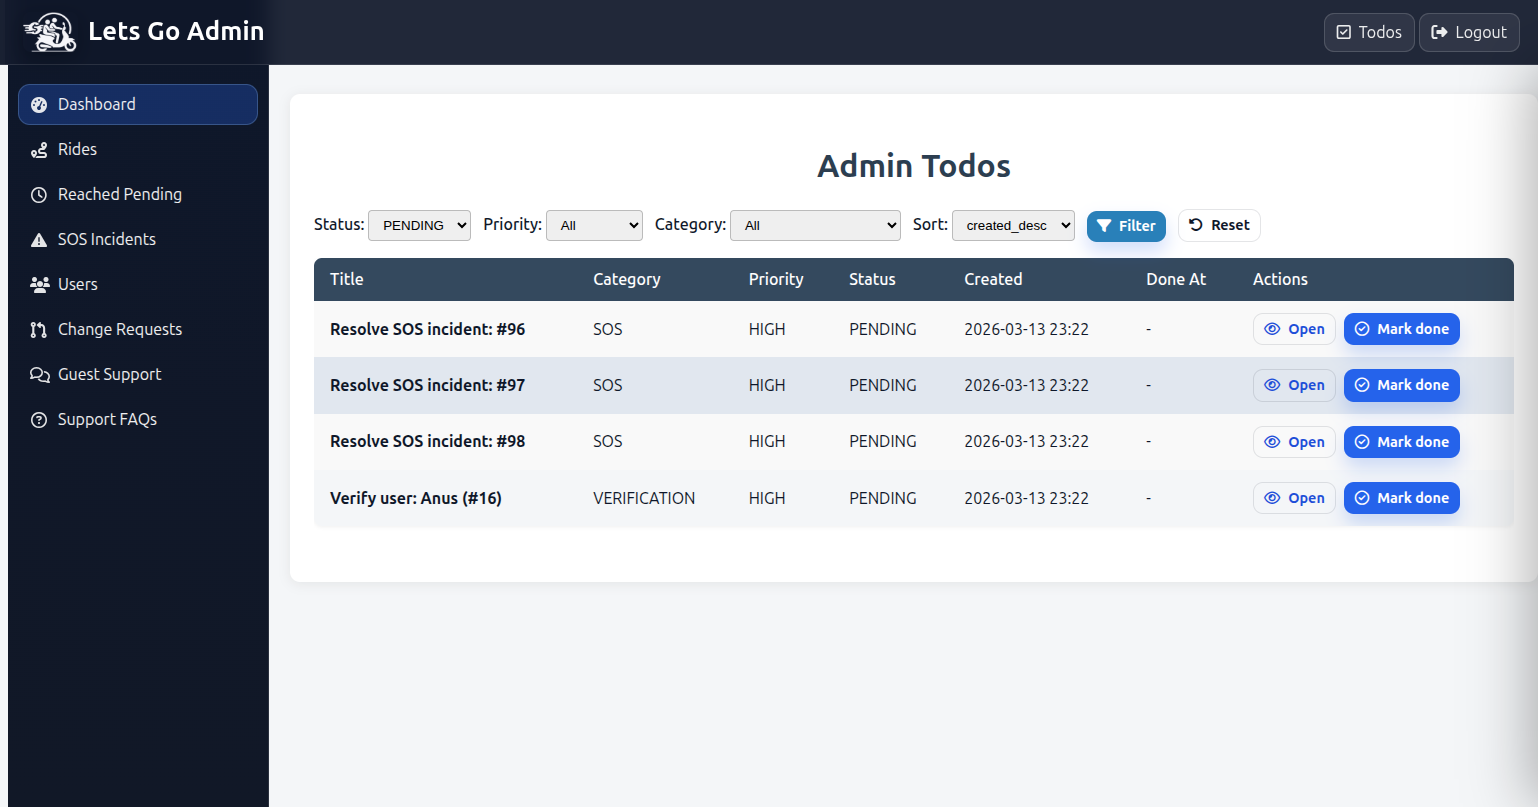
\includegraphics[width=0.85\textwidth,keepaspectratio]{assets/app screenshot/dashboard images/administration-todos.png}}
\caption{Admin Todos Inbox}
\end{figure}

\subsubsection{Screen 50: Support FAQs Management}
Purpose: Control FAQ entries for use by support and bot responses.

The components include the FAQ list, add/edit form, and the publish/update control.

Functional Flow: Admin adds / edits FAQs and these are made available to user support flows.

Backend Integration: Utilizes FAQ CRUD views backed by administration database models.

Validation/Security: Only Admins can edit FAQs and input is checked for validation before adding content.

\begin{figure}[H]
\centering
\fbox{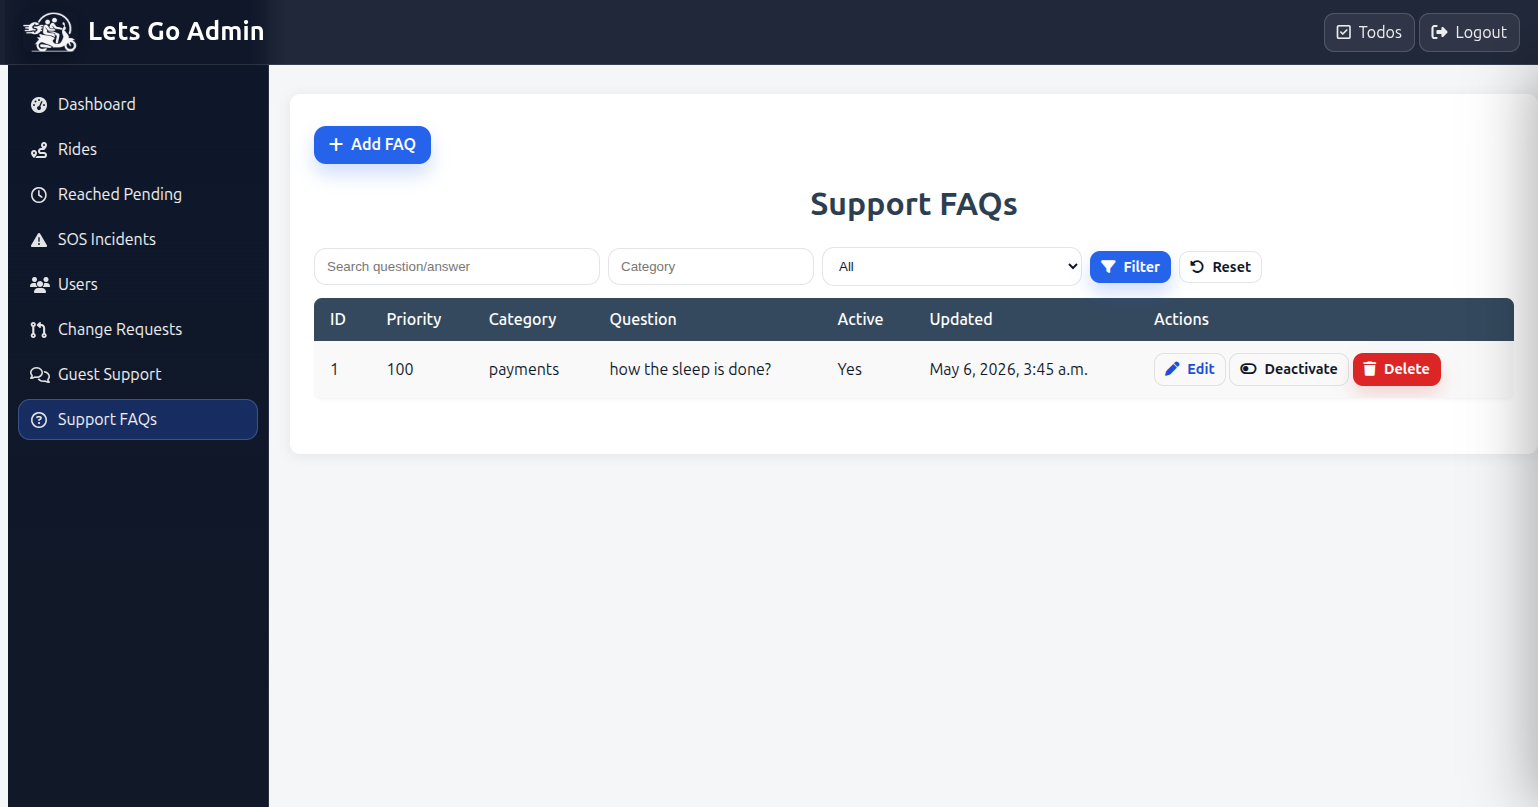
\includegraphics[width=0.85\textwidth,keepaspectratio]{assets/app screenshot/dashboard images/administration-support-faqs.png}}
\caption{Support FAQs Management}
\end{figure}

\subsubsection{Screen 51: Guest Support Users List}
The purpose of this is to be able to see the guests and to deal with support conversations without the need to have complete registration.

Components: Guest user list, access to chat thread, and support response tools.

Functional Flow: Admin is able to choose a guest user and then open the chat thread for resolution.

Guest List and chat templates are linked with the support message store, which powers Backend Integration.

Validation/Security: Guest threads are protected in accordance with the guest identity and only accessible for authorized admin sessions.

\begin{figure}[H]
\centering
\fbox{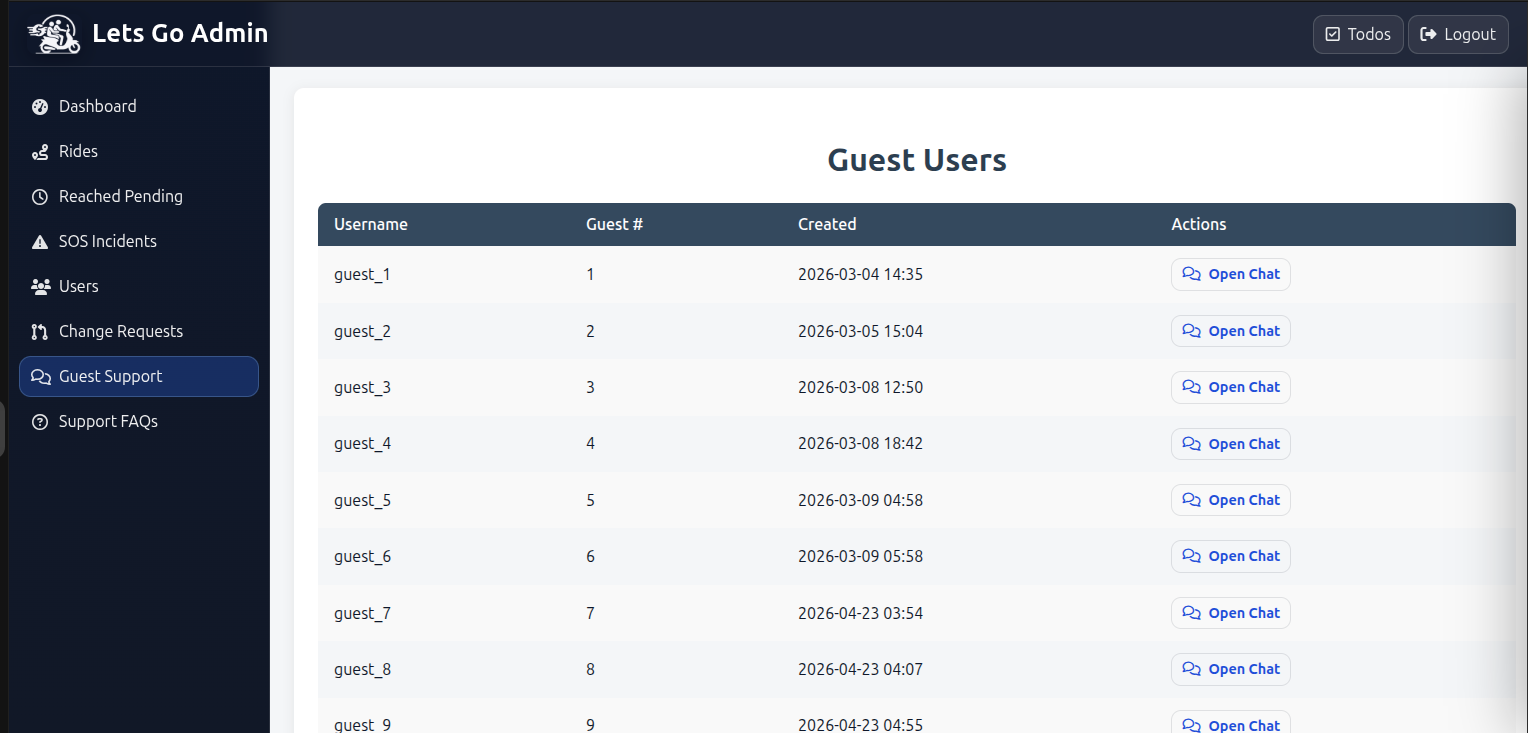
\includegraphics[width=0.85\textwidth,keepaspectratio]{assets/app screenshot/dashboard images/Guest-Users.png}}
\caption{Guest Support Users List}
\end{figure}

\subsection{Navigation Flow Diagram}

The route and the general navigation flow of the mobile app is shown below.

\begin{figure}[H]
\centering
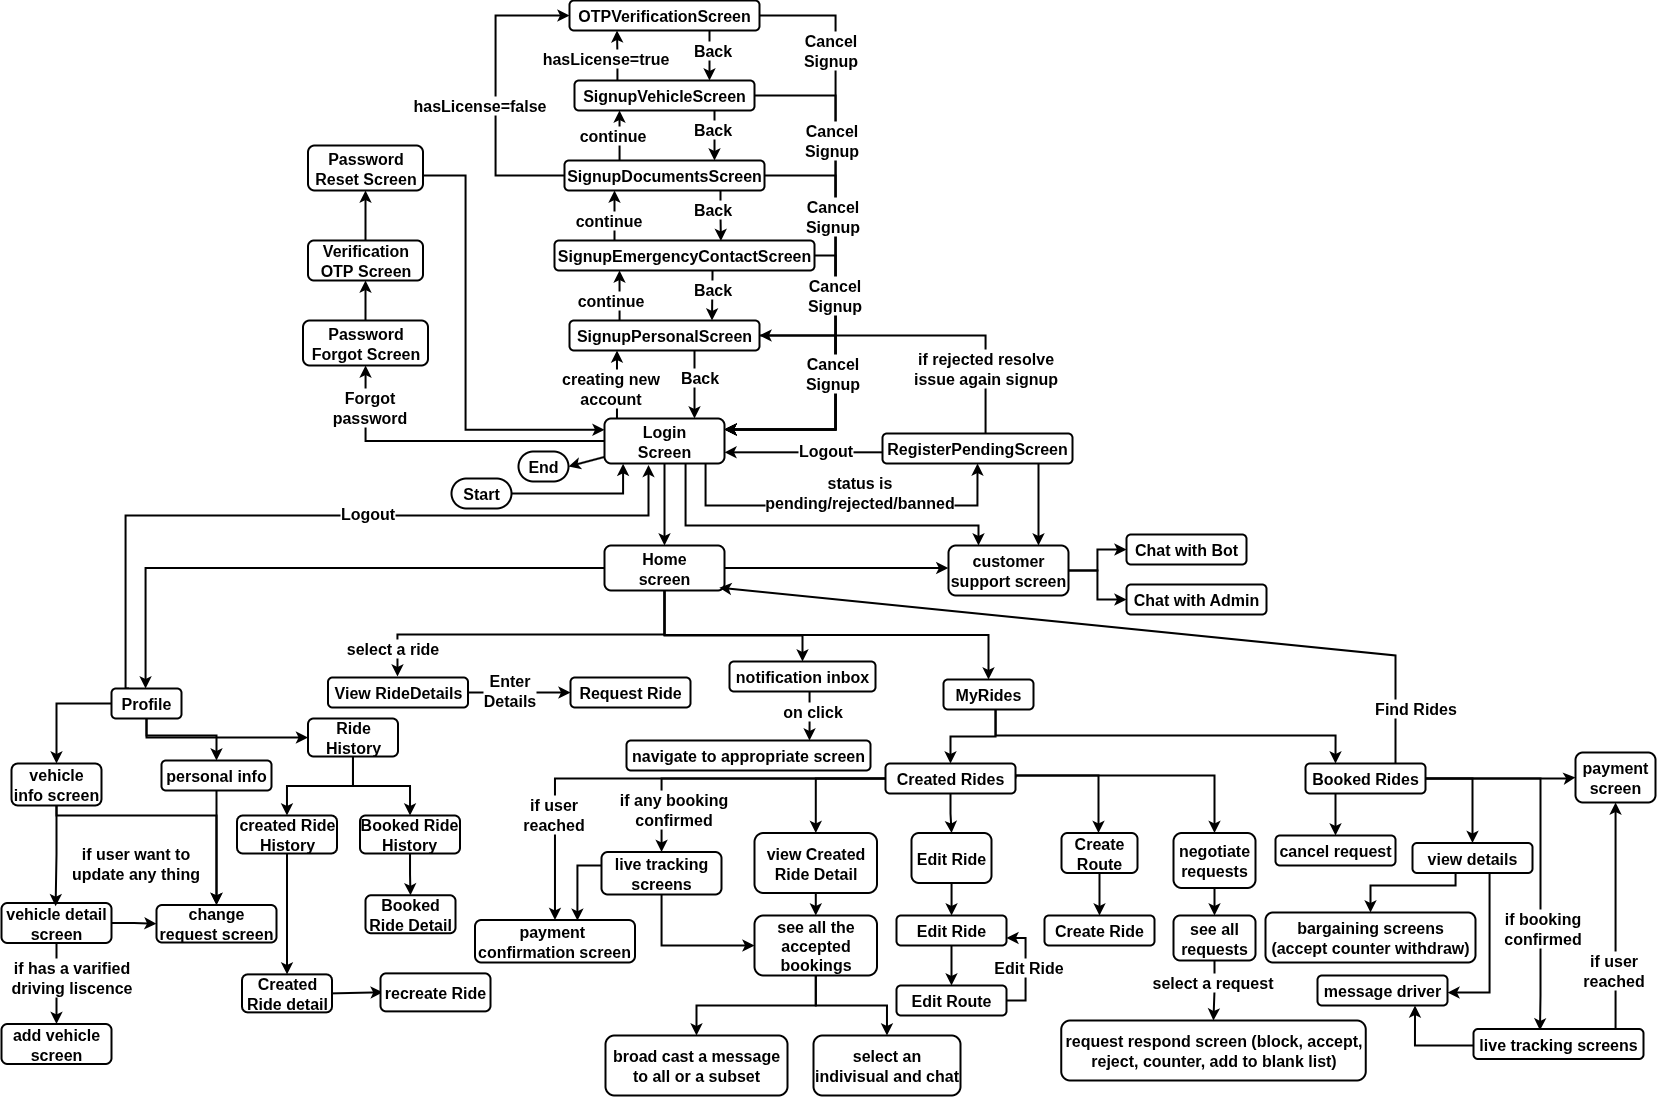
\includegraphics[width=0.9\textwidth,keepaspectratio,height=0.8\textheight]{assets/db_diagrams/navigation_flow_diagram.png}
\caption{Application Navigation Flow}
\end{figure}

\subsection{Responsiveness and Performance}

The Flutter app is made responsive to different screen sizes with the help of:

Wrapping layouts with -\texttt{LayoutBuilder} and -\texttt{MediaQuery} to adapt layouts.
- \texttt{Expanded} and \texttt{Flexible} widgets for dynamic spacing.
- Tabler layout for larger screens.

Performance considerations include:

- Long ride lists with pagination.
Document and media upload caching.
Efficient state updates to avoid unnecessary rebuilds.
Refreshed locations periodically rather than persistent socket connections.

% -------------------------------------------------
% 5.6 Deployment
% -------------------------------------------------

\section{Deployment}

The Django backend and Admin pages are deployed via cloud hosting and the database and file storage are managed via Supabase.

\begin{table}[htbp]
\centering
\caption{Deployment Details}
\begin{tabularx}{\textwidth}{|p{3cm}|p{3cm}|X|}
\hline
\textbf{Component} & \textbf{Platform} & \textbf{URL/Details} \\
\hline
Backend API & Vercel & Django backend deployment with function-based views and path-based routing \\
\hline
Database & Supabase & Managed PostgreSQL database used for application data \\
\hline
Admin Web Panel & Vercel & Django template-based Admin pages deployed with the backend \\
\hline
Mobile App (Android) & GitHub Releases & Direct APK distribution for testers and users \\
\hline
Storage & Supabase Storage & Object storage for user documents and media \\
\hline
\end{tabularx}
\end{table}

CI/CD: These are integrated with the hosting platform and run via GitHub Actions:

Backend \& Admin Pages: Automatically deploy changes to the hosting environment when they're merged to the \texttt{main} branch.
- Mobile App: Automated build pipelines to build release-ready APKs, uploaded to GitHub Releases.

\textbf{Security Measures:}

- HTTPS Encryption: TLS protects data that is being transferred.
- Authentication: authenticated user access via Django sessions.
Environment Security: Sensitive credentials and API keys are stored in environment variables and not hard-coded.

% -------------------------------------------------
% Chapter Summary
% -------------------------------------------------

\section*{Chapter Summary}

The chapter discussed the development environment, the core modules of the Lets Go Ride Sharing App system, the algorithms, external integrations and user interface implementation, and deployment of the Lets Go Ride Sharing App system. It is implemented in a modular fashion described in Chapter 4 and is implemented consistently using Django, Flutter, PostgreSQL on Supabase, and Supabase Storage.

Key achievements include:

- Documenting use cases and translating them to working code paths and back end workflows.
- Session based authentication and OTP based verification flows.
Ride creation, booking, negotiation, chat, tracking and SOS support.
Responsive mobile app that has screens that adapt to the screen being used and template-based Admin Pages.
Cloud deployment with Vercel, Supabase and GitHub Releases.

The system developed is now ready for a complete test and evaluation, which will be explored in the next chapter.
